\documentclass[12pt,oneside]{../../sfsuthesis} 
 
\RequirePackage{standalone}
\usepackage[draft]{../../MAThesisOutputFormat}
%====================%
% Packages 
%====================%
%\usepackage{accents}  % Better accents. I'm not using this
\usepackage{enumitem} % Better labels
%\usepackage[explicit]{titlesec}
\usepackage[normalem]{ulem}     % Thing
\usepackage{stackrel} % Stack text nicely
\usepackage{xcolor}   % Nicer Colors

%====================%
% Re-Define 
%====================%
% Sort out the true phi
\def \badphi {\phi}
\def \phi {\varphi}

%====================%
% New Commands 
%====================%
%% Nice Letters
% Blackboard Bold
\newcommand{\R}{\mathbb{R}}
\newcommand{\Z}{\mathbb{Z}}
\newcommand{\bbS}{\mathbb{S}}
% Fancy Math Cal Letters
\newcommand{\I}{\mathcal{I}}
\newcommand{\J}{\mathcal{J}}
\newcommand{\cL}{\mathcal{L}}
\newcommand{\cF}{\mathcal{F}}
% The hipster letters
\newcommand{\sM}{\mathsf{M}}
\newcommand{\bSigma}{\boldsymbol{\Sigma}}
\newcommand{\ow}{\overline{w}}
\newcommand{\oP}{\overline{P}}
\newcommand{\oQ}{\overline{Q}}
\newcommand{\ochi}{\overline{\chi}}
%% Math Operators
\newcommand{\Cub}{\operatorname{Cub}}
\newcommand{\oCub}{\overline{\Cub}}
\newcommand{\Vol}{\operatorname{Vol}}
\newcommand{\oVol}{\overline{\Vol}}
\newcommand{\MVol}{\operatorname{MVol}}
%% Math Symbols
\newcommand{\cl}{\mathrm{cl}}
\newcommand{\rk}{\mathrm{rk}}
\newcommand{\Inn}{\mathrm{Inn}}
\newcommand{\cone}{\mathrm{cone}}

%====================%
% Theorem Environs
%====================%
\newtheorem{dummy}{}[section]
\theoremstyle{definition}
\newtheorem*{Result}{Main Result}

%====================%
% Draft Helpers
%====================%
% \todo : Make a box with todo comments
\newcommand{\todo}[1]{\par \noindent
    \framebox{\begin{minipage}[c]{0.95 \textwidth}
            \textcolor{red}{TO DO:}
            #1 \end{minipage}}\par}
\usepackage[backend=biber,style=alphabetic]{biblatex}
\addbibresource{../../thesis.bib}

\begin{document}

\chapter{Bergman Fans and their Normal Complexes}
As we continue our tour of various branches of mathematics, we arrive at geometry.
The primary goal of this chapter is to develop the final segment of our bridge connecting some geometric object back to the Chow ring, and then showing how we can generate log-concave sequences with these objects.
To get there we will provide a quick primer on polyhedral geometry and a classic theorem of convex geometry that generates log-concave sequences.
Then we will introduce a geometric object associated to a matroid, the Bergman fan, and show how we can use them to make some new objects called normal complexes.

\section{A Little Polyhedral Geometry, as a Treat}
Really, the basic building blocks we will be using are not that weird.
It is geometry, we are going to be using some sort of shapes living in some kind of space.
We must admit, however, that we personally struggle visualizing the higher dimensional objects at play, and so must fall back on formalism.

This section is a short crash course on basic elements of polyhedral geometry.
Our treatment of this topic will often parallel that in Ziegler's ``Lectures on Polytopes'' \cite{zieglerLecturesPolytopes1995}, which we recommend for those who'd like a little more depth than presented here.

\subsection{The Cone Zone}
We are going to be using two fundamental kinds of convex shapes, polytopes and cones.
As a reminder, a convex object is one where if you pick any two points in it, the line connecting those points never leaves the shape.
We can, and will, state this formally.
\begin{definition}[Convexity]\label{def:convex}
    Let \( K \subseteq \R^n \).
    We call \( K \) \emph{convex} if for every \( p, q \in K \), we have
    \[
        [p, q] \subseteq K,
    \]
    where \( [p, q] = \{ \lambda p + (1 - \lambda) q \; | \; 0 \leq \lambda \leq 1 \} \) is the line segment between \( p \) and \( q \).
\end{definition}

\begin{figure}[H]

    \begin{subfigure}[t]{0.5\textwidth}
        \centering
        \begin{tikzpicture}[scale=0.7]
            \draw[thick, fill=SeaGreen, opacity=0.5] (-2,-2) -- (-2,2) -- (2,2) -- (2,-2) -- cycle;

            \node[circle, fill=MidnightBlue, scale=0.5] (A) at (1.2, -1.55) {};
            \node[circle, fill=MidnightBlue, scale=0.5] (B) at (-1.8, 0.2) {};
            \draw[thick, MidnightBlue] (A) -- (B);
        \end{tikzpicture}

    \end{subfigure}
    \begin{subfigure}[t]{0.5\textwidth}
        \centering
        \begin{tikzpicture}[scale=0.7]
            \pgfmathsetmacro{\ct}{3} % distance center to tip
            \pgfmathsetmacro{\cc}{\ct*sin(18)/sin(126)} % distance center to corner (sine rule)
            % star
            \draw[thick, fill=Goldenrod, opacity=0.5] (0,0)
            +(90-0*36:\ct) coordinate(T1)
            foreach[evaluate=\x as \nc using int((\x+1)/2),   % number for corner coordinates
                    evaluate=\x as \nt using int((\x+1)/2+1)] % number for tip coordinates
            \x in {1,3,...,9}{
                    -- +(90-\x*36:\cc) coordinate(C\nc) -- +({90-(\x+1)*36}:\ct) coordinate(T\nt)}
            -- cycle;
            % \node[above=1cm] at (T1) {star only};
            % star
            % \draw[ultra thick] (7,0)
            %     +(90-0*36:\ct) coordinate(T1)
            %     foreach[evaluate=\x as \nc using int((\x+1)/2),   % number for corner coordinates
            %             evaluate=\x as \nt using int((\x+1)/2+1)] % number for tip coordinates
            %         \x in {1,3,...,9}{
            %         -- +(90-\x*36:\cc) coordinate(C\nc) -- +({90-(\x+1)*36}:\ct) coordinate(T\nt)}
            %     -- cycle;
            % % the rest
            % \draw[ultra thick] (C2) -- (C3) -- (C4);
            % \draw[ultra thick,fill=green] (T5) -- (C1) -- (C4) -- cycle;
            % \draw[ultra thick,fill=green] (C4) -- (C1) -- (T2) -- (C2) -- (C4);

            % \node[above=1cm] at (T1) {complete};
            \node[circle, fill=red, scale=0.5] (A) at (-1.2, -1.55) {};
            \node[circle, fill=red, scale=0.5] (B) at (-1.6, 0.5) {};
            \draw[thick, red] (A) -- (B);
        \end{tikzpicture}
    \end{subfigure}
    \caption{Everyone's first pair of convex and non-convex shapes.}
\end{figure}

While there are generally a few ways one could define polytope and cone, we will use a definition based on construction using some finite collection of points.
In brief, a polytope is a \emph{convex hull} of finitely many points and a cone is the \emph{conic combination} of finitely many generating vectors.
Let's make this formal.
\begin{definition}[Polytope]\label{def:polytope}
    Let \( P \subseteq \R^n \).
    We say \( P \) is a \emph{polytope} if it is the convex hull of some finite set of points \( x_1, x_2, \dots, x_k \).
    That is to say \( P \) is a polytope if
    \[
        P = \conv(\{x_1, \dots, x_k\}),
    \]
    where
    \[
        \conv(\{x_1, \dots, x_k\}) = \left\{ \lambda_1 x_1 + \lambda_2 x_2 + \cdots + \lambda_k x_k \; \middle| \; \lambda_i \geq 0, \sum_{i=0}^k \lambda_i = 1 \right\}
    \]
    is the convex hull of \( x_1, x_2, \dots, x_k \).
\end{definition}
An astute reader may notice that our shorthand for line segment above, \( [x, y] \), is in fact just \( \conv(\{x,y\}) \).
Towards some intuition, we may think of the convex hull as the smallest convex shape that contains all of its generating points.
In two dimensions we like to think of this as stretching a rubber band around a bunch of points and letting it constrict around them.
\begin{figure}[H]
    \begin{subfigure}[t]{0.3\textwidth}
        \centering
        \begin{tikzpicture}[scale=.72]

            \node[circle, fill=Black, scale=0.7] (A) at (-1, -3) {};
            % \node[circle, fill=Black, scale=0.7] (B) at (-0.5, -1.5) {};
            \node[circle, fill=Black, scale=0.7] (C) at (1, 3) {};
            \draw[ultra thick, Black] (A) -- (C);
        \end{tikzpicture}
        \subcaption*{A 1-dimensional polytope}
    \end{subfigure}
    \begin{subfigure}[t]{0.3\textwidth}
        \centering
        \begin{tikzpicture}[scale=.85]

            \node[circle, fill=Black, scale=0.7] (A) at (-1, -1) {};
            \node[circle, fill=Black, scale=0.7] (B) at (-1.5, 0.25) {};
            \node[circle, fill=Black, scale=0.7] (C) at (-1.5, 2) {};
            \node[circle, fill=Black, scale=0.7] (D) at (1, 4) {};
            \node[circle, fill=Black, scale=0.7] (E) at (2, -.3) {};

            \draw[ultra thick, fill=CornflowerBlue, opacity=0.7] (A.center) -- (B.center) -- (C.center) -- (D.center) -- (E.center) -- cycle;

            \node[circle, fill=Black, scale=0.7] (A) at (-1, -1) {};
            \node[circle, fill=Black, scale=0.7] (B) at (-1.5, 0.25) {};
            \node[circle, fill=Black, scale=0.7] (C) at (-1.5, 2) {};
            \node[circle, fill=Black, scale=0.7] (D) at (1, 4) {};
            \node[circle, fill=Black, scale=0.7] (E) at (2, -.3) {};
        \end{tikzpicture}
        \subcaption*{A 2-dimensional polytope}
    \end{subfigure}
    \begin{subfigure}[t]{0.4\textwidth}
        \centering
        \tdplotsetmaincoords{75}{55}
        \begin{tikzpicture}[tdplot_main_coords,line join=round, scale=.95]

            \path
            (0,0,0)  coordinate (O)
            (0,0,4) coordinate (Z)
            (4,0,0)  coordinate (X)
            (0,4,0)  coordinate (Y);


            \draw[ultra thick,fill=Cyan, opacity=0.5] (O) -- (Y) -- (Z) -- cycle;
            \draw[ultra thick,fill=NavyBlue, opacity=0.5] (O) -- (X)  -- (Y) -- cycle;
            \draw[ultra thick,fill=Gray, opacity=0.5] (O) -- (X)  -- (Z) -- cycle;
            \draw[ultra thick,fill=White, opacity=0.5] (X) -- (Y)  -- (Z) -- cycle;

            \foreach \p in {O,X,Y,Z}
            \draw[fill=black] (\p) circle (2.5pt);

        \end{tikzpicture}
        \subcaption*{A 3-dimensional polytope}
    \end{subfigure}
    \caption{A sampling of polytopes; note that we have highlighted the vertices, which are the minimal set of points that generate the polytope.}
\end{figure}

We will use a similar definition for cones.
They are built out of a finite collection of generating vectors.
\begin{definition}[Cone]\th\label{def:cone}
    Let \( C \subseteq \R^n \).
    We call \( C \) a \emph{cone} if it is the conic combination of finitely many vectors \( x_1, x_2, \dots, x_k \).
    We write this
    \[
        C = \cone(\{x_1, \dots, x_k\}),
    \]
    where
    \[
        \cone(\{x_1, \dots, x_k\}) = \left\{ \lambda_1 x_1 + \lambda_2 x_2 + \cdots + \lambda_k x_k \; \middle| \; \lambda_i \geq 0 \right\}
    \]
    is the conic combinations of \( x_1, x_2, \dots, x_k \).

\end{definition}
Unlike the more familiar notion of cones, these are not pointed cylinders.
\begin{figure}[H]
    \centering
    \begin{subfigure}[t]{0.3\textwidth}
        \centering
        \begin{tikzpicture}[scale=2]

            % Axes 
            \draw[->, Black] (0,0) -- (1,0);
            \draw[->, Black] (0,0) -- (-1,0);
            \draw[->, Black] (0,0) -- (0,1);
            \draw[->, Black] (0,0) -- (0,-1);
            \node[circle, fill=Black, inner sep=0.81] at (0,0) {};

            % Cone
            \draw[fill=CarnationPink, opacity=0.6] (0,0) -- (-0.55, 1.32) -- (-1.26,0.525) -- cycle;
            \draw[->, Black, ultra thick] (0,0) -- (-.5, 1.2);
            \draw[->, Black, ultra thick] (0,0) -- (-1.2,.5);

            \node[circle, fill=Black, inner sep=1.2] at (0,0) {};
        \end{tikzpicture}

        \subcaption*{A 2-dimensional cone}
    \end{subfigure}
    \begin{subfigure}[t]{0.3\textwidth}
        \centering
        \tdplotsetmaincoords{68}{55}
        \begin{tikzpicture}[scale=3,tdplot_main_coords]

            \draw [<->] (-0.5,0,0) -- (1,0,0) node [right] {};
            \draw [<->] (0,-0.5,0) -- (0,1,0) node [left] {};
            \draw [<->] (0,0,-0.5) -- (0,0,1) node [left] {};

            \coordinate (O) at (0,0,0);
            \coordinate (A) at (0.75, 0.75, 0);
            \coordinate (B) at (0.0, 0.75, 0.8);
            \coordinate (C) at (0.7, 0.5, 0.2);

            \node[circle, fill=Black, inner sep=0.81] at (O) {};

            \draw[draw=blue!20,fill=CarnationPink,fill opacity=0.3]  (O)-- (A) -- (B) -- cycle;
            \draw[draw=blue!20,fill=CarnationPink,fill opacity=0.4]  (O)-- (A) -- (C) -- cycle;
            \draw[draw=blue!20,fill=Gray,fill opacity=0.3]  (O)-- (A) -- (C) -- cycle;
            \draw[draw=blue!20,fill=CarnationPink,fill opacity=0.4]  (O)-- (B) -- (C) -- cycle;
            \draw[draw=blue!20,fill=White,fill opacity=0.3]  (O)-- (B) -- (C) -- cycle;

            \draw[ultra thick, ->] (O) -- (A);
            \draw[ultra thick, ->] (O) -- (B);
            \draw[ultra thick, ->] (O) -- (C);

            \node[circle, fill=Black, inner sep=1.2] at (0,0) {};
        \end{tikzpicture}

        \subcaption*{A 3-dimensional cone \\ (generated by 3 vectors)}
    \end{subfigure}
    \begin{subfigure}[t]{0.3\textwidth}
        \centering
        \tdplotsetmaincoords{79}{35}
        \begin{tikzpicture}[scale=3,tdplot_main_coords]

            \draw [<->] (-1,0,0) -- (0.5,0,0) node [right] {};
            \draw [<->] (0,-1,0) -- (0,0.5,0) node [left] {};
            \draw [<->] (0,0,-1) -- (0,0,0.5) node [left] {};

            \coordinate (O) at (0,0,0);
            \coordinate (A) at (-0.75, -0.75, 0);
            \coordinate (B) at (0.0, -0.75, -0.8);
            \coordinate (C) at (-0.7, -0.5, 0.2);
            \coordinate (D) at (0.3, -1.2, -0.3);


            % \node at (A) {A};
            % \node at (B) {B};
            % \node at (C) {C};
            % \node at (D) {D};

            \node[circle, fill=Black, inner sep=0.81] at (O) {};


            \draw[draw=blue!20,fill=CarnationPink,fill opacity=0.3]  (O)-- (A) -- (C) -- cycle;
            \draw[draw=blue!20,fill=White,fill opacity=0.5]  (O)-- (A) -- (C) -- cycle;
            \draw[draw=blue!20,fill=CarnationPink,fill opacity=0.3]  (O)-- (A) -- (B) -- cycle;
            \draw[draw=blue!20,fill=Gray,fill opacity=0.3]  (O)-- (A) -- (B) -- cycle;
            \draw[draw=blue!20,fill=CarnationPink,fill opacity=0.3]  (O)-- (B) -- (D) -- cycle;
            \draw[draw=blue!20,fill=CarnationPink,fill opacity=0.3]  (O)-- (C) -- (D) -- cycle;

            % \draw[draw=blue!20,fill=CarnationPink,fill opacity=0.4]  (O)-- (A) -- (C) -- cycle;
            % \draw[draw=blue!20,fill=Gray,fill opacity=0.3]  (O)-- (A) -- (C) -- cycle;

            % \draw[draw=blue!20,fill=CarnationPink,fill opacity=0.4]  (O)-- (B) -- (C) -- cycle;
            % \draw[draw=blue!20,fill=White,fill opacity=0.3]  (O)-- (B) -- (C) -- cycle;

            \draw[ultra thick, ->,opacity=0.5] (O) -- (D);
            \draw[ultra thick, ->,opacity=0.5, color=CarnationPink] (O) -- (D);
            \draw[ultra thick, ->] (O) -- (A);
            \draw[ultra thick, ->] (O) -- (B);
            \draw[ultra thick, ->] (O) -- (C);

            \node[circle, fill=Black, inner sep=1.2] at (0,0) {};
        \end{tikzpicture}

        \subcaption*{A 3-dimensional cone \\ (generated by 4 vectors)}
    \end{subfigure}
    \caption{Some examples of cones.}
    \label{fig:cones}
\end{figure}
We notice that conic combinations are essentially the span of the generating vectors but taking only non-negative linear combinations.
Indeed, one can quickly confirm that \( \cone(\{x_1, \dots, x_k\}) \subseteq \Span(\{x_1, \dots, x_k\}) \).

\subsection{Points vs. Vectors: An Affine Primer}
We have been, and will be going forward, using the words ``points'' and ``vectors'' quite interchangeably.
Is there a difference?
Strictly speaking, yes there is.
Points imply elements of an affine space, while vectors, naturally, are elements of a vector space.
Affine spaces can be thought of as vector spaces where the \( 0 \)-vector is ``forgotten'', but are otherwise essentially the same collection of ``stuff''.
Mathematicians love to make multiple objects out of the same basic thing by giving (or losing) some extra structure.

This poses a slight problem since we want to refer to the dimension of our polytopes and cones (and already have been in figures), but a notion of dimension usually relies on a vector space.
To settle a notion of dimension here, we first want to define what an affine span (also called an affine hull) is.
\begin{definition}[Affine Span]\th\label{def:affineSpan}
    Let \( S \subseteq \R^d \).
    The \emph{affine span} of \( S \) is the set
    \[
        \aff(S) = \left\{ \sum_{i=1}^k \lambda_k x_k \; \middle| \; k > 0,\,  x_i \in S,\, \sum_{i=1}^k \lambda_i = 1 \right\}.
    \]
\end{definition}
The affine span of some set will be something that looks like a linear subspace, but might not include the origin.
In fact if \( 0 \in S \), then the affine span and our more traditional linear span coincide exactly.
The insight here then is that we could always translate our affine span so that it includes the origin.
Once we have a linear subspace we can just use the linear algebra definition of dimension.
\begin{definition}[Affine Dimension]\th\label{def:affineDimension}
    Given any set \( S \subseteq \R^d \), designate some element \( x_0 \in S \).
    The \emph{dimension} of \( S \) is
    \[
        \dim(S) = \dim\bigl( \aff(S)-x_0 \bigr),
    \]
    where, on the right-hand side, \( \dim \) is the standard notion of dimension of a subspace in linear algebra.
\end{definition}
We are overloading our notation a bit, but we promise this mostly reduces cognitive load.
This also goes to explain our switching between ``point'' or ``vector''.
Since our cones are defined to always include \( 0 \), affine and linear terms align, so we are safe to just think in terms of vector spaces.
Indeed, for cones we will always just write \( \Span(\cC) \) in lieu of \( \aff(\cC) \).

Dimension will mostly align with intuition, but it is good to have the definitions at hand if ever in doubt.
Early chapters of \cite{zieglerLecturesPolytopes1995} and \cite{grunbaumConvexPolytopes2003} both provide a good treatment of affine spaces.

\subsection{The Minkowski Sum}
Now that we have the basic shapes down we need be able to make new ones out of existing ones.
The two general strategies here will be to combine them in to new ones and to break them down.
We will start with learning how we can add shapes together, using what we call the Minkowski sum.
\begin{definition}[Minkowski Sum]\th\label{def:MinkowskiSum}
    Let \( P, Q \subseteq \R^n \).
    The \emph{Minkowski sum} of \( P \) and \( Q \) is given by
    \[
        P + Q = \left\{ p + q \; \middle| \; p \in P, q \in Q \right\}.
    \]
\end{definition}
Sit with this definition for a few moments to confirm the Minkowski sum does have the nice properties of sums we normally expect.
It is commutative, associative, and has an identity in \( \{ 0 \} \).
An additional feature of the definition is that the empty set has the property that for any \( P \subseteq \R^n \)
\[
    P + \emptyset = \emptyset.
\]

A way to think about the Minkowski sum is ``smearing'' one shape around the other.
You pick some point in either shape, then drag it along the boarder of the other shape in the sum.
This makes more sense with a picture.
\begin{figure}[H]
    \centering
    \def\radius{.5cm}
    \begin{tikzpicture}[scale=2]
        \coordinate (a) at (0,0);
        \coordinate (b) at (3,-1);
        \coordinate (c) at (2,2);

        \coordinate (a_out) at ($(a)!\radius!-90:(b)$);
        \coordinate (a_in) at ($(a)!\radius!90:(b)$);
        \coordinate (b_out) at ($(b)!\radius!-90:(b)$);

        % Draw circles! 
        \foreach \nd in {a, b, c} {\draw[dashed, thick, color=Emerald, opacity=1] (\nd) circle (\radius);}

        % Fill side rectangles
        \draw[draw=none, fill=Emerald, opacity=0.3] ($(a)!\radius!-90:(b)$) coordinate (AtB) -- ($(b)!\radius!90:(a)$) coordinate (BtA) -- (b) -- (a) -- cycle;
        \draw[draw=none, fill=Emerald, opacity=0.3] ($(a)!\radius!90:(c)$) coordinate (AtC) -- ($(c)!\radius!-90:(a)$) coordinate (CtA) -- (c) -- (a) -- cycle;
        \draw[draw=none, fill=Emerald, opacity=0.3] ($(b)!\radius!-90:(c)$) coordinate (BtC) -- ($(c)!\radius!90:(b)$) coordinate (CtB) -- (c) -- (b) -- cycle;

        % Fill missing angles and outer part of circle
        \draw pic [draw=none, fill=Emerald, opacity=0.3, angle radius=2*\radius] {angle=AtC--a--AtB};
        \draw pic [draw, ultra thick, angle radius=2*\radius] {angle=AtC--a--AtB};

        \draw pic [draw=none, fill=Emerald, opacity=0.3, angle radius=2*\radius] {angle=BtA--b--BtC};
        \draw pic [draw, ultra thick, angle radius=2*\radius] {angle=BtA--b--BtC};

        \draw pic [draw=none, fill=Emerald, opacity=0.3, angle radius=2*\radius] {angle=CtB--c--CtA};
        \draw pic [draw, ultra thick,  angle radius=2*\radius] {angle=CtB--c--CtA};
        % Draw lines connecting circles
        \draw[ultra thick] ($(a)!\radius!-90:(b)$) -- ($(b)!\radius!90:(a)$) ($(b)!\radius!-90:(c)$) -- ($(c)!\radius!90:(b)$) ($(c)!\radius!-90:(a)$) -- ($(a)!\radius!90:(c)$) ($(a)!\radius!-90:(b)$);

        % Fill inner triangle
        \draw[dashed, thick, fill=RoyalBlue, opacity=0.3] (a) -- (b) -- (c) -- cycle;

        % Put a dot in the center of each circle
        \foreach \nd in {a, b, c} {\node[circle, fill=Black, opacity=1, scale=0.2] at (\nd) {};}
    \end{tikzpicture}
    \caption{A visual representation of a Minkowski sum of a triangle and a circle.}
\end{figure}
This is a helpful visual intuition, but it may take a moment to be convinced that, up to translation, the resulting shape doesn't depend on either the shape you choose to smear or the choice of point in that shape.

With the Minkowski sum, we can finally define a general polyhedron.
\begin{definition}[Polyhedron]\th\label{def:polyhedron}
    Let \( P \subseteq \R^n \). We call \( P \) a \emph{polyhedron} if
    \[
        P = \conv(\{x_1, \dots, x_k\}) + \cone(\{y_1, \dots, y_\ell\}),
    \]
    for some finite sets \( \{x_1, \dots, x_k\}, \{y_1, \dots, y_\ell\} \subseteq \R^n \).
\end{definition}
A polyhedron is the result of the Minkowski sum of a polytope and a cone.
Clearly every polytope and cone are polyhedra themselves, as \( \conv(\{0\}) = \cone(\{0\}) = \{ 0 \} \).
Polyhedra are not necessarily bounded, which may seem a bit unusual to those who have seen the word in other contexts.
Moreover, all bounded polyhedra are polytopes, which is not necessarily obvious, but useful to keep in mind.
We will mostly be focused on either polytopes or cones at any one time, but having a more general object that includes both makes our definitions going forward cleaner.

\subsection{About Faces}
Given a polyhedron \( P \), we also get a whole family of polyhedra, the faces of \( P \).
Let's first go back to simpler times.
If we were to think of a cube, we would have faces of the cube as the 2 dimensional squares that make up the sides.
We'd then call the line segments where any two of those squares meet \textit{edges} and the points where those edges meet \textit{vertices}.
\begin{figure}[H]
    \centering
    \begin{subfigure}{0.24\textwidth}
        \newcommand{\Depth}{2}
        \newcommand{\Height}{2}
        \newcommand{\Width}{2}
        \begin{tikzpicture}
            \coordinate (O) at (0,0,0);
            \coordinate (A) at (0,\Width,0);
            \coordinate (B) at (0,\Width,\Height);
            \coordinate (C) at (0,0,\Height);
            \coordinate (D) at (\Depth,0,0);
            \coordinate (E) at (\Depth,\Width,0);
            \coordinate (F) at (\Depth,\Width,\Height);
            \coordinate (G) at (\Depth,0,\Height);

            \draw[Red,fill=Red!80] (O) -- (C) -- (G) -- (D) -- cycle;% Bottom Face
            \draw[Red,fill=Red!30] (O) -- (A) -- (E) -- (D) -- cycle;% Back Face
            \draw[Red,fill=Red!10] (O) -- (A) -- (B) -- (C) -- cycle;% Left Face
            \draw[Red,fill=Red!20,opacity=0.8] (D) -- (E) -- (F) -- (G) -- cycle;% Right Face
            \draw[Red,fill=Red!20,opacity=0.6] (C) -- (B) -- (F) -- (G) -- cycle;% Front Face
            \draw[Red,fill=Red!20,opacity=0.8] (A) -- (B) -- (F) -- (E) -- cycle;% Top Face

            %% Following is for debugging purposes so you can see where the points are
            %% These are last so that they show up on top
            %\foreach \xy in {O, A, B, C, D, E, F, G}{
            %    \node at (\xy) {\xy};
            %}
        \end{tikzpicture}
    \end{subfigure}
    \begin{subfigure}{0.24\textwidth}
        \newcommand{\Depth}{2}
        \newcommand{\Height}{2}
        \newcommand{\Width}{2}
        \begin{tikzpicture}
            \coordinate (O) at (0,0,0);
            \coordinate (A) at (0,\Width,0);
            \coordinate (B) at (0,\Width,\Height);
            \coordinate (C) at (0,0,\Height);
            \coordinate (D) at (\Depth,0,0);
            \coordinate (E) at (\Depth,\Width,0);
            \coordinate (F) at (\Depth,\Width,\Height);
            \coordinate (G) at (\Depth,0,\Height);

            \fill[Gray,fill=Gray!50, opacity=0.5] (O) -- (C) -- (G) -- (D) -- cycle;% Bottom Face
            \fill[Gray,fill=Gray!10, opacity=0.5] (O) -- (A) -- (E) -- (D) -- cycle;% Back Face
            \fill[Gray,fill=Gray!5, opacity=0.5] (O) -- (A) -- (B) -- (C) -- cycle;% Left Face
            \fill[Gray,fill=Gray!8,opacity=0.4] (D) -- (E) -- (F) -- (G) -- cycle;% Right Face
            \fill[Gray,fill=Gray!10,opacity=0.2] (C) -- (B) -- (F) -- (G) -- cycle;% Front Face
            \fill[Gray,fill=Gray!10,opacity=0.4] (A) -- (B) -- (F) -- (E) -- cycle;% Top Face

            \draw[Red,fill=Red!70,opacity=0.75] ($ (O) + (0,-0.25*\Width, 0) $) -- ($ (C) + (0,-0.25*\Width, 0) $) -- ($ (G) + (0,-0.25*\Width, 0) $) -- ($ (D) + (0,-0.25*\Width, 0) $) -- cycle;% Bottom Face
            % \draw[Red,fill=Red!30] (O) -- (A) -- (E) -- (D) -- cycle;% Back Face
            \draw[Red,fill=Red!30] ($ (O) + (0.25\Depth,0.25*\Width, 0) $) -- ($ (A) + (0.25\Depth,0.25*\Width, 0) $) -- ($ (E) + (0.25\Depth,0.25*\Width, 0) $) -- ($ (D) + (0.25\Depth,0.25*\Width, 0) $) -- cycle;% Back Face
            % \draw[Red,fill=Red!10] (O) -- (A) -- (B) -- (C) -- cycle;% Left Face
            \draw[Red,fill=Red!30] ($ (O) + (-0.25\Depth,0*\Width, 0) $) -- ($ (A) + (-0.25\Depth,0*\Width, 0) $) -- ($ (B) + (-0.25\Depth,0*\Width, 0) $) -- ($ (C) + (-0.25\Depth,0*\Width, 0) $) -- cycle;% Left Face
            % \draw[Red,fill=Red!20,opacity=0.8] (D) -- (E) -- (F) -- (G) -- cycle;% Right Face
            \draw[Red,fill=Red!30,opacity=0.8] ($ (D) + (0.2\Depth,0*\Width, 0) $) -- ($ (E) + (0.2\Depth,0*\Width, 0) $) -- ($ (F) + (0.2\Depth,0*\Width, 0) $) -- ($ (G) + (0.2\Depth,0*\Width, 0) $) -- cycle;% Right Face
            \draw[Red,fill=Red!20,opacity=0.6] (C) -- (B) -- (F) -- (G) -- cycle;% Front Face
            % \draw[Red,fill=Red!20,opacity=0.8] (A) -- (B) -- (F) -- (E) -- cycle;% Top Face
            \draw[Red,fill=Red!30,opacity=0.8] ($ (A) + (0*\Depth,0.2*\Width, 0*\Height) $) -- ($ (B) + (0*\Depth,0.2*\Width, 0*\Height) $) -- ($ (F) + (0*\Depth,0.2*\Width, 0*\Height) $) -- ($ (E) + (0*\Depth,0.2*\Width, 0*\Height) $) -- cycle;% Right Face

            %% Following is for debugging purposes so you can see where the points are
            %% These are last so that they show up on top
            %\foreach \xy in {O, A, B, C, D, E, F, G}{
            %    \node at (\xy) {\xy};
            %}
        \end{tikzpicture}
    \end{subfigure}
    \begin{subfigure}{0.24\textwidth}
        \newcommand{\Depth}{2}
        \newcommand{\Height}{2}
        \newcommand{\Width}{2}
        \begin{tikzpicture}
            \coordinate (O) at (0,0,0);
            \coordinate (A) at (0,\Width,0);
            \coordinate (B) at (0,\Width,\Height);
            \coordinate (C) at (0,0,\Height);
            \coordinate (D) at (\Depth,0,0);
            \coordinate (E) at (\Depth,\Width,0);
            \coordinate (F) at (\Depth,\Width,\Height);
            \coordinate (G) at (\Depth,0,\Height);

            \coordinate(Down) at (0, -0.1*\Width, 0);
            \coordinate(Up) at (0, 0.1*\Width, 0);
            \coordinate(Right) at (0.1*\Depth, 0, 0);
            \coordinate(Left) at (-0.1*\Depth, 0, 0);
            \coordinate(Forward) at (0, 0, 0.1*\Height);
            \coordinate(Back) at (0, 0, -0.1*\Height);

            \fill[ Gray,fill=Gray!80, opacity=0.5] (O) -- (C) -- (G) -- (D) -- cycle;% Bottom Face
            \fill[Gray,fill=Gray!50, opacity=0.5] (O) -- (A) -- (E) -- (D) -- cycle;% Back Face
            \fill[Gray,fill=Gray!10, opacity=0.5] (O) -- (A) -- (B) -- (C) -- cycle;% Left Face
            \fill[Gray,fill=Gray!20,opacity=0.4] (D) -- (E) -- (F) -- (G) -- cycle;% Right Face
            \fill[Gray,fill=Gray!20,opacity=0.2] (C) -- (B) -- (F) -- (G) -- cycle;% Front Face
            \fill[Gray,fill=Gray!20,opacity=0.4] (A) -- (B) -- (F) -- (E) -- cycle;% Top Face

            % Back Face
            \draw[Red, ultra thick, opacity=0.5] ($ (O) + (Back) + (Left) $) -- ($ (A) + (Back) + (Left) $);
            \draw[Red, ultra thick, opacity=0.5] ($ (A) + (Back) + (Up) $) -- ($ (E) + (Back) + (Up) $);
            \draw[Red, ultra thick, opacity=0.5] ($ (E) + (Back) + (Right) $) -- ($ (D) + (Back) + (Right) $);
            \draw[Red, ultra thick, opacity=0.5] ($ (D) + (Back) + (Down) $) -- ($ (O) + (Back) + (Down) $);
            % Left Side
            \draw[Red, ultra thick, opacity=0.5] ($ (A) + (Up) + (Left) $) -- ($ (B) + (Up) + (Left) $);
            \draw[Red, ultra thick, opacity=0.5] ($ (O) + (Left) + (Down) $) -- ($ (C) + (Left) + (Down) $);
            % Right Side
            \draw[Red, ultra thick, opacity=0.5] ($ (E)  + (Up) + (Right) $) -- ($ (F)  + (Up) + (Right) $);
            \draw[Red, ultra thick, opacity=0.5] ($ (G) + (Down) + (Right) $) -- ($ (D) + (Down) + (Right) $);
            % Front Face
            \draw[Red, ultra thick, opacity=0.5] ($ (C) + (Forward) + (Left) $) -- ($ (B) + (Forward) + (Left) $);
            \draw[Red, ultra thick, opacity=0.5] ($ (B) + (Forward) + (Up) $) -- ($ (F) + (Forward) + (Up) $);
            \draw[Red, ultra thick, opacity=0.5] ($ (F) + (Forward) + (Right) $) -- ($ (G) + (Forward) + (Right) $);
            \draw[Red, ultra thick, opacity=0.5] ($ (G) + (Forward) + (Down) $) -- ($ (C) + (Forward) + (Down) $);

            % \draw[Red, thick] ($ (B) + -0.1*(B) $) -- ($ (C) + -0.1*(C) $);
            % \draw[Red, thick] ($ (B) + -0.1*(B) $) -- ($ (C) + -0.1*(C) $);
            % \draw[Red, thick] ($ (B) + -0.1*(B) $) -- ($ (C) + -0.1*(C) $);
            % \draw[Red, thick] ($ (B) + -0.1*(B) $) -- ($ (C) + -0.1*(C) $);

            %% Following is for debugging purposes so you can see where the points are
            %% These are last so that they show up on top
            %\foreach \xy in {O, A, B, C, D, E, F, G}{
            %    \node at (\xy) {\xy};
            %}
        \end{tikzpicture}
    \end{subfigure}
    \begin{subfigure}{0.24\textwidth}
        \newcommand{\Depth}{2}
        \newcommand{\Height}{2}
        \newcommand{\Width}{2}
        \begin{tikzpicture}
            \coordinate (O) at (0,0,0);
            \coordinate (A) at (0,\Width,0);
            \coordinate (B) at (0,\Width,\Height);
            \coordinate (C) at (0,0,\Height);
            \coordinate (D) at (\Depth,0,0);
            \coordinate (E) at (\Depth,\Width,0);
            \coordinate (F) at (\Depth,\Width,\Height);
            \coordinate (G) at (\Depth,0,\Height);

            \draw[Gray,fill=Gray!50, opacity=0.5] (O) -- (C) -- (G) -- (D) -- cycle;% Bottom Face
            \draw[Gray,fill=Gray!10, opacity=0.5] (O) -- (A) -- (E) -- (D) -- cycle;% Back Face
            \draw[Gray,fill=Gray!5, opacity=0.5] (O) -- (A) -- (B) -- (C) -- cycle;% Left Face
            \draw[Gray,fill=Gray!8,opacity=0.4] (D) -- (E) -- (F) -- (G) -- cycle;% Right Face
            \draw[Gray,fill=Gray!10,opacity=0.2] (C) -- (B) -- (F) -- (G) -- cycle;% Front Face
            \draw[Gray,fill=Gray!10,opacity=0.4] (A) -- (B) -- (F) -- (E) -- cycle;% Top Face

            \node[circle, fill=Red, opacity=0.5, minimum size=5pt, inner sep=0] at (O) {};
            \node[circle, fill=Red, opacity=0.5, minimum size=5pt, inner sep=0] at (A) {};
            \node[circle, fill=Red, opacity=0.5, minimum size=5pt, inner sep=0] at (B) {};
            \node[circle, fill=Red, opacity=0.5, minimum size=5pt, inner sep=0] at (C) {};
            \node[circle, fill=Red, opacity=0.5, minimum size=5pt, inner sep=0] at (D) {};
            \node[circle, fill=Red, opacity=0.5, minimum size=5pt, inner sep=0] at (E) {};
            \node[circle, fill=Red, opacity=0.5, minimum size=5pt, inner sep=0] at (F) {};
            \node[circle, fill=Red, opacity=0.5, minimum size=5pt, inner sep=0] at (G) {};

            % \draw[Red,fill=Red!80] (O) -- (C) -- (G) -- (D) -- cycle;% Bottom Face
            % \draw[Red,fill=Red!30] (O) -- (A) -- (E) -- (D) -- cycle;% Back Face
            % \draw[Red,fill=Red!10] (O) -- (A) -- (B) -- (C) -- cycle;% Left Face
            % \draw[Red,fill=Red!20,opacity=0.8] (D) -- (E) -- (F) -- (G) -- cycle;% Right Face
            % \draw[Red,fill=Red!20,opacity=0.6] (C) -- (B) -- (F) -- (G) -- cycle;% Front Face
            % \draw[Red,fill=Red!20,opacity=0.8] (A) -- (B) -- (F) -- (E) -- cycle;% Top Face

            %% Following is for debugging purposes so you can see where the points are
            %% These are last so that they show up on top
            %\foreach \xy in {O, A, B, C, D, E, F, G}{
            %    \node at (\xy) {\xy};
            %}
        \end{tikzpicture}
    \end{subfigure}
    \caption{The faces of a cube; note that the full cube is a face of itself (as is the empty set, which we drew as accurately as possible).}
\end{figure}
If this sounds familiar then the intuition for our more general notion of the face of a polyhedron is not far.
Back in our world of polyhedral geometry, we know that a cube is a polyhedron and that each of those squares, lines, and points are also themselves polyhedra.
Informally, we use the term face to describe all these ``sub-polyhedra'' that make up the boundary of a polyhedron.
\begin{definition}[Face]\th\label{def:face}
    Let \( P \subseteq \R^n \) be a polyhedron and \( \bigcdot \) be the standard dot product.
    The \emph{hyperplane} normal to a vector \( x \in \R^n \) at distance \( b \in \R \)  is given by
    \[
        \HP_x(b) = \left\{ v \in \R^n \; \middle| \; v \bigcdot x = b \right\}.
    \]
    The lower half-space is given by
    \[
        \LH_x(b) = \left\{ v \in \R^n \; \middle| \; v \bigcdot x \leq b \right\}.
    \]
    Then \( F \subseteq P \) is a \emph{face} of \( P \) if there exist \( x, b \) such that
    \[
        F = P \cap \HP_x(b)
    \]
    where
    \begin{gather*}
        P \subseteq \LH_x(b).
    \end{gather*}

\end{definition}
Some notable quirks of this definition are that when \( x = 0 \) and \( b \in \R_{\geq 0} \),
\[
    \HP_0(b) \cap P = P.
\]
So \( P \) is a face of itself by our definition.
Likewise, if we pick \( x = 0 \) and \( b < 0 \), then
\[
    \HP_x(b) \cap P = \emptyset,
\]
which means the empty set too is a face of any polyhedron \( P \).
As a note, we do still call the \( 0 \)-dimensional faces vertices, while the generic term for a \( (d - 1) \)-dimensional face of a \( d \)-dimensional polyhedron is a \textit{facet}.
\begin{figure}[H]
    \centering
    \tdplotsetmaincoords{70}{110} % Adjust the viewing angle
    \begin{tikzpicture}[tdplot_main_coords, scale=1.5]

        % Cube
        \draw[thick] (0,0,0) -- (2,0,0) -- (2,2,0) -- (0,2,0) -- cycle;
        \draw[thick] (0,0,2) -- (2,0,2) -- (2,2,2) -- (0,2,2) -- cycle;
        \draw[thick] (0,0,0) -- (0,0,2);
        \draw[thick] (2,0,0) -- (2,0,2);
        \draw[thick] (2,2,0) -- (2,2,2);
        \draw[thick] (0,2,0) -- (0,2,2);

        % Plane
        \fill[gray!50, opacity=0.5] (-0.75,-0.75,0) -- (2.75,-0.75,0) -- (2.75,2.75,0) -- (-0.75,2.75,0) -- cycle;

        % Intersection edge
        \draw[ultra thick, Red, fill=Red, opacity=0.5] (0,0,0) -- (2,0,0) -- (2,2,0) -- (0,2,0) -- cycle;

    \end{tikzpicture}
    \caption{Example of specifying a facet of our cube with a plane.}
\end{figure}

From our cube intuition exercise, there are some things about faces that we would hope to generalize to our broader notion of faces.
We will state these without proof, and again refer to the early chapters of \cite{zieglerLecturesPolytopes1995}.
\begin{proposition}
    Given a polyhedron \( P \), then
    \begin{itemize}
        \item if \( F \subseteq P \) is a face of \( P \), then \( F \) is a polyhedron,
        \item if \( F \subseteq P \), then any face \( F' \subseteq F \) of \( F \) is also a face of \( P \),
        \item if \( F_1, F_2 \subseteq P \) are two faces of \( P \), then \( F_1 \cap F_2 \) is a face of \( P \)
    \end{itemize}
\end{proposition}
It is worth remembering that the intersection of two faces can be empty, but \( \emptyset \subseteq P \) is a face of any polyhedron \( P \), so this causes no issues.

We will often write \( F \preceq P \) to mean \( F \) is a face of \( P \).
Indeed, the relation ``is a face of'' induces a partial ordering on the set of all faces of \( P \).
Even stronger, using the propositions above it follows that the relation induces a lattice (where the join of two faces is the smallest face containing both).

\section{The Geometer's Guide to Generating Log-Concave Sequences}
Having developed our shapes, we are going to need to measure them somehow.
Specifically, we want their volume.
As with the rest of this chapter so far, we are going to take something that most people can intuitively grasp for 3-dimensional shapes and generalize.
Not only do we need volume for arbitrary dimensional polytopes, we need something called the mixed volume which gives us some sense of volume of multiple shapes.
This work however will allow us to introduce a classic result of convex geometry that relates geometry to log-concave sequences.

From here, the last few background points can no longer be readily found in Ziegler.
Instead, we turn to Rolf Schneider's ``Convex Bodies'' \cite{schneiderConvexBodiesBrunn2013} as a comprehensive reference.

\subsection{Volume Functions}
We again need to formalize something that most of us would take for granted.
The notion of volume is intuitive enough for 3-dimensional shapes, we however need to generalize this to all dimensions.
We will actually only need the volume of polytopes, so we restrict our notion of volume to just them.
\begin{definition}[Volume Function]
    A \emph{volume function} is a map
    \[
        \Vol_n\,:\; \{\text{polytopes in \( \R^n \)}\} \to \R_{\geq 0}
    \]
    such that
    \begin{enumerate}
        \item \( \Vol_n(P) > 0 \) when \( \dim(P) = n \) and \( \Vol_n(P) = 0 \) when \( \dim(P) < n \),
        \item \( \Vol_n(P) =  \Vol_n(P+v) \) for any \( v \in \R^n \),
        \item when \( P \cup Q \) is a polytope,
              \[
                  \Vol_n(P \cup Q) = \Vol(P) + \Vol_n(Q) - \Vol(P \cap Q),
              \]
        \item for any linear map \( T \in \Hom(\R^n, \R^n) \),
              \[
                  \Vol_n(T(P)) = |\det(T)|\Vol_n(P).
              \]
    \end{enumerate}
\end{definition}
When the dimension is unambiguous, we will write \( \Vol_n \) as simply \( \Vol \).
This definition does not uniquely specify a single ``volume function'', but rather a family of maps that all differ from one another by a constant multiple.
We can differentiate different volume maps by their value on a single fixed polytope.
For example, in \( 2 \)-dimensions, our ``standard'' volume function is the one that takes the unit square to \( 1 \).
\begin{figure}[H]
    \centering
    \begin{subfigure}[t]{0.45\textwidth}
        \centering
        \newcommand{\GridDim}{3}
        \begin{tikzpicture}[scale=1, baseline=(O)]
            %% Grid 
            \foreach \x in {0,...,\GridDim} {
                    \foreach \y in {0,...,\GridDim} {
                            \fill[color=Black, opacity=0.25] (\x,\y) circle (0.1);
                        }
                }
            % Marked points 
            \coordinate (O) at (0, 0);

            % Unit Square
            \filldraw[thick, color=Black!75, fill=SeaGreen!75, fill opacity=0.65] (0,0) -- (0,1) -- (1, 1) -- (1, 0) -- cycle;
            \fill[fill=SeaGreen!50, fill opacity=0.25] (0,0) -- (0,1) -- (1, 1) -- (1, 0) -- cycle;
            \draw[thick, color=Black!75] (0,0) -- (0,1) -- (1, 1) -- (1, 0) -- cycle;

            \node at (0.5, 0.5) {\( 1 \)};

            % 
            \filldraw[thick, color=Black!75, fill=SeaGreen!75, fill opacity=0.65] (2,2) -- +(0,1) -- +(1, 0) -- cycle;
            \filldraw[dashed, color=SeaGreen!95, fill=SeaGreen!75, fill opacity=0.15] (2,2) -- ++(0,1) -- ++(1, 0) -- ++(0, -1) -- cycle;
            \draw[thick, color=Black!75] (2,2) -- +(0,1) -- +(1, 0) -- cycle;

            \node at (2.25, 2.35) {\( \frac{1}{2} \)};

        \end{tikzpicture}
    \end{subfigure}
    \begin{subfigure}[t]{0.45\textwidth}
        \centering
        \newcommand{\GridDim}{3}
        \begin{tikzpicture}[scale=1, baseline=(O)]
            %% Grid 
            \foreach \x in {0,...,\GridDim} {
                    \foreach \y in {0,...,\GridDim} {
                            \fill[color=Black, opacity=0.25] (\x,\y) circle (0.1);
                        }
                }
            % Marked points 
            \coordinate (O) at (0, 0);

            % Fill Big Shape
            \fill[color=SeaGreen!75, fill opacity=0.65 ] (0,0) -- (0,3) -- (1,3) -- (3,1) -- (3,0) -- cycle;

            \foreach \y in {0, 1, 2}{
                    \filldraw[dashed, color=SeaGreen!95, fill=SeaGreen!75, fill opacity=0.15] (0,\y) -- ++(0,1) -- ++(1, 0) -- ++(0, -1) -- cycle;
                }

            \foreach \y in {0, 1, 2}{
                    \filldraw[dashed, color=SeaGreen!95, fill=SeaGreen!75, fill opacity=0.15] (1,\y) -- ++(0,1) -- ++(1, 0) -- ++(0, -1) -- cycle;
                }

            \foreach \y in {0, 1}{
                    \filldraw[dashed, color=SeaGreen!95, fill=SeaGreen!75, fill opacity=0.15] (2,\y) -- ++(0,1) -- ++(1, 0) -- ++(0, -1) -- cycle;
                }

            \filldraw[dashed, color=SeaGreen!95, fill=SeaGreen!75, fill opacity=0.15] (2,0) -- ++(0,1) -- ++(1, 0) -- ++(0, -1) -- cycle;


            \draw[thick, color=Black!75] (0,0) -- (0,3) -- (1,3) -- (3,1) -- (3,0) -- cycle;

            \node at (1.5,0.5) {\( 7 \) };
        \end{tikzpicture}
    \end{subfigure}
    \caption{Examples of using our ``standard'' volume.}
\end{figure}
Any two volume functions only differ by a constant.
Another reasonable choice of volume is \textit{simplicial volume}.
Given a vector space with a basis \( \{e_1, \dots, e_n\} \), the associated simplicial volume is the volume map such that
\[
    \Vol_n \big(\conv(\{0, e_1, e_2, \dots, e_n\})\big) = 1.
\]
\begin{figure}[H]
    \centering
    \begin{subfigure}[t]{0.45\textwidth}
        \centering
        \newcommand{\GridDim}{3}
        \begin{tikzpicture}[scale=1, baseline=(O)]
            %% Grid 
            \foreach \x in {0,...,\GridDim} {
                    \foreach \y in {0,...,\GridDim} {
                            \fill[color=Black, opacity=0.25] (\x,\y) circle (0.1);
                        }
                }
            % Marked points 
            \coordinate (O) at (0, 0);

            % Unit Square
            \filldraw[thick, color=Black!75, fill=SeaGreen!75, fill opacity=0.65] (0,0) -- (0,1) -- (1, 1) -- (1, 0) -- cycle;

            \filldraw[dashed, color=Violet!95, fill=Violet!75, fill opacity = 0.15] (0,0) -- (0,1) -- (1, 0) -- cycle;
            \filldraw[dashed, color=Violet!95, fill=Violet!75, fill opacity = 0.15] (1,1) -- (0,1) -- (1, 0) -- cycle;

            \draw[thick, color=Black!75] (0,0) -- (0,1) -- (1, 1) -- (1, 0) -- cycle;



            \node at (0.5, 0.5) {\( 2 \)};

            % Triangle
            \filldraw[thick, color=Black!75, fill=SeaGreen!75, fill opacity=0.65] (2,2) -- +(0,1) -- +(1, 0) -- cycle;
            \filldraw[dashed, color=Violet!95, fill=Violet!75, fill opacity = 0.15] (2,2) -- +(0,1) -- +(1, 0) -- cycle;
            \draw[thick, color=Black!75] (2,2) -- +(0,1) -- +(1, 0) -- cycle;

            \node at (2.25, 2.35) {\( 1 \)};

        \end{tikzpicture}
    \end{subfigure}
    \begin{subfigure}[t]{0.45\textwidth}
        \centering
        \newcommand{\GridDim}{3}
        \begin{tikzpicture}[scale=1, baseline=(O)]
            %% Grid 
            \foreach \x in {0,...,\GridDim} {
                    \foreach \y in {0,...,\GridDim} {
                            \fill[color=Black, opacity=0.25] (\x,\y) circle (0.1);
                        }
                }
            % Marked points 
            \coordinate (O) at (0, 0);

            % Fill Big Shape
            \fill[color=SeaGreen!75, fill opacity=0.65 ] (0,0) -- (0,3) -- (1,3) -- (3,1) -- (3,0) -- cycle;

            \foreach \y in {0, 1, 2}{
                    \filldraw[dashed, color=Violet!95, fill=Violet!75, fill opacity=0.15] (0,\y) -- +(0,1) -- +(1, 0) -- cycle;
                }

            \foreach \y in {0, 1, 2}{
                    \filldraw[dashed, color=Violet!95, fill=Violet!75, fill opacity=0.15] (0,\y+1) -- ++(1,0) -- +(0, -1);
                    \filldraw[dashed, color=Violet!95, fill=Violet!75, fill opacity=0.15] (1,\y) -- +(0,1) -- +(1, 0) -- cycle;
                }

            \foreach \y in {0, 1}{
                    \filldraw[dashed, color=Violet!95, fill=Violet!75, fill opacity=0.15] (1,\y+1) -- ++(1,0) -- +(0, -1);
                    \filldraw[dashed, color=Violet!95, fill=Violet!75, fill opacity=0.15] (2,\y) -- +(0,1) -- +(1, 0) -- cycle;
                }

            % \filldraw[dashed, color=Violet!95, fill=Violet!75, fill opacity=0.15] (1,1) -- ++(1,0) -- +(0, -1);

            % \filldraw[dashed, color=Violet!95, fill=Violet!75, fill opacity=0.15] (2,0) -- +(0,1) -- +(1, 0) -- cycle;

            \filldraw[dashed, color=Violet!95, fill=Violet!75, fill opacity=0.15] (2,1) -- ++(1,0) -- +(0, -1);


            \draw[thick, color=Black!75] (0,0) -- (0,3) -- (1,3) -- (3,1) -- (3,0) -- cycle;

            \node at (1.5,0.5) {\( 14 \) };
        \end{tikzpicture}
    \end{subfigure}
    \caption{Example of simplicial volume in \( \R^2 \); notice it differs from our ``standard'' by a factor of 2.}
\end{figure}
\subsection{Mixed Volume}
While volume functions may not be too odd a concept we will use it to define a less widely known function.
Given any \( 2 \) polytopes in \( \R^2 \), or \( 3 \) polytopes in \( \R^3 \), or more generally \( n \) polytopes in \( \R^n \), we want a map from these collections of polytopes to \( \R_{\geq 0} \) that is, in some sense, consistent with volume and Minkowski summation.
We call this map the mixed volume function.
\begin{definition}[Mixed Volume -- Characterization]\th\label{def:mixedVolume}
    The \emph{mixed volume function} is a map \( \MVol_n \) from ordered multisets \( P_1, P_2, \dots, P_n \subseteq \R^n \) of polytopes to \( \mathbb{R}_{\geq 0} \), such that it has the following properties:
    \begin{enumerate}
        \item \( \MVol_n(P, P, \dots, P) = \Vol_n(P) \), for any polytope \( P \subseteq \R^n \),
        \item \( \MVol_n \) is symmetric in all arguments, and
        \item \( \MVol_n \) is multilinear with respect to scaling and Minkowski addition.
    \end{enumerate}
\end{definition}
Just like volume, we will often just notate this as \( \MVol \) when safe to do so.
The proof that such a function exists and is indeed uniquely defined by these properties can be found in \cite{schneiderConvexBodiesBrunn2013}.
While this characterization is useful, it goes very little of the way to actually telling us what mixed volumes are.

Consider two polytopes \( P, Q \subseteq \R^2 \).
We could ask ourselves, what is the volume of the Minkowski sum of \( P \) and \( Q \).
We could be more ambitious and even allow ourselves to scale \( P \) and \( Q \) by arbitrary values.
That is to say, let us consider the volume
\[
    \Vol_2(\lambda P + \mu Q),
\]
for some \( \lambda, \mu \in \R \).
Answering this question is where mixed volumes appear as something more concrete.
While not immediately obvious, this volume can always be expressed as a polynomial in \( \lambda \) and \( \mu \), and mixed volumes appear as coefficients of these polynomials.
We can consider an example.
\begin{figure}[H]
    \centering
    \begin{subfigure}[t]{0.3\textwidth}
        \centering
        \begin{tikzpicture} [scale=0.8,
                axis/.style={-, black, very thin},
                vector/.style={-stealth, black, thin},
                flat vector/.style={-stealth, red, very thick},
                vector guide/.style={dashed, red, very thick}]

            \coordinate (0) at (-2, 1) {};
            \coordinate (1) at (-1, 1) {};
            \coordinate (2) at (-2, 0) {};
            \coordinate (3) at (-1, 0) {};
            \coordinate (4) at (0, 2) {};
            \coordinate (5) at (0, 0) {};
            \coordinate (6) at (2, 0) {};
            \coordinate[label=below:\( P \)] (7) at (-1.5, -0.25) {};
            \coordinate[label=below:\( Q \)] (8) at (1, -0.25) {};

            \draw [fill=Cyan, fill opacity=0.5] (0.center) -- (1) -- (3) -- (2) -- cycle;
            \draw [fill=Red, fill opacity=0.5] (4) -- (5) -- (6) -- cycle;
        \end{tikzpicture}
    \end{subfigure}
    \hfill
    \begin{subfigure}[t]{0.3\textwidth}
        \centering
        \begin{tikzpicture} [scale=0.8,
                axis/.style={-, black, very thin},
                vector/.style={-stealth, black, thin},
                flat vector/.style={-stealth, red, very thick},
                vector guide/.style={dashed, red, very thick}]

            \coordinate (0) at (-3, 1) {};
            \coordinate (1) at (-2, 1) {};
            \coordinate (2) at (-3, 0) {};
            \coordinate (3) at (-2, 0) {};

            \coordinate (A) at (-3, 2) {};
            \coordinate (B) at (-1, 2) {};
            \coordinate (C) at (-1, 0) {};

            \coordinate (4) at (0, 2) {};
            \coordinate (5) at (0, 0) {};
            \coordinate (6) at (2, 0) {};

            \coordinate (D) at (0, 3) {};
            \coordinate (E) at (3, 0) {};

            \coordinate[label=below:\( \lambda P \)] (7) at (-2.1, -0.25) {};
            \coordinate[label=below:\( \mu Q \)] (8) at (1.4, -0.25) {};

            \draw [fill=Cyan, fill opacity=0.5] (0.center) -- (1) -- (3) -- (2) -- cycle;
            \draw [fill=Cyan, fill opacity=0.2] (0) -- (A) -- (B) -- (C) -- (3) -- (1) -- cycle;

            \draw [fill=Red, fill opacity=0.5] (4) -- (5) -- (6) -- cycle;
            \draw [fill=Red, fill opacity=0.2] (4) -- (D) -- (E) -- (6) --cycle;
        \end{tikzpicture}
    \end{subfigure}
    \hfill
    \begin{subfigure}[t]{0.35\textwidth}
        \centering
        \begin{tikzpicture} [scale=1.0,
                axis/.style={-, black, very thin},
                vector/.style={-stealth, black, thin},
                flat vector/.style={-stealth, red, very thick},
                vector guide/.style={dashed, red, very thick}]

            \coordinate (0) at (-1, -1) {};
            \coordinate (1) at (-1, 0.5) {};
            \coordinate (2) at (0.5, 0.5) {};
            \coordinate (3) at (0.5, -1) {};

            \coordinate (4) at (-1, 3) {};
            \coordinate (5) at (0.5, 3) {};
            \coordinate (6) at (3, 0.5) {};
            \coordinate (7) at (3, -1) {};

            \coordinate [label=below:\( \lambda P + \mu Q \)] (8) at (1, -1.4) {};

            \draw [fill=Cyan, fill opacity=0.6] (0) -- (1) -- (2) -- (3) -- cycle;
            \draw [fill=Red, fill opacity=0.6] (2) -- (5) -- (6) -- cycle;

            \draw [fill=Lavender, fill opacity=0.4] (1) -- (2) -- (5) -- (4) -- cycle;
            \draw [fill=Lavender, fill opacity=0.4] (2) -- (6) -- (7) -- (3) -- cycle;

        \end{tikzpicture}
    \end{subfigure}
    \caption*{ \( \Vol(\lambda P + \mu Q) = \MVol(P, P)\lambda^2 + 2\MVol(P, Q)\lambda \mu + \MVol(Q,Q) \mu^2 \)}

    \caption{The mixed volume appears in the coefficients of the volume polynomial;\\
        recall that \( \MVol(P, P) = \Vol(P) \).}
\end{figure}
This idea generalizes to any dimension, and can be taken as another definition of mixed volume.
\begin{definition}[Mixed Volume -- As Coefficients]
    Let  \( P_1, P_2, \dots, P_\ell \subseteq \R^n \) be polytopes.
    The function
    \[
        f(\lambda_1, \lambda_2, \dots, \lambda_\ell)  = \Vol(\lambda_1 P_1 + \lambda_2 P_2 + \cdots + \lambda_\ell P_\ell), \quad \lambda_j \geq 0
    \]
    is a homogeneous polynomial of degree \( n \).
    It can be written symmetrically as
    \[
        f(\lambda_1, \dots, \lambda_\ell) = \sum_{\mathclap{j_1, j_2, \dots, j_n = 1}}^{\ell} \MVol(P_{j_1}, \dots, P_{j_n})\lambda_{j_1} \cdots \lambda_{j_n}.
    \]
    The coefficient associated to \( \lambda_{j_1} \cdots \lambda_{j_n} \) is the \emph{mixed volume} of \( P_{j_1}, \dots, P_{j_n} \).

\end{definition}
Of course, you could start with either definition of mixed volume and derive the other, they are equivalent after all.

At this point, one may begin to wonder why this section should even exist.
We seem to have gone rather far afield with our geometry lesson.
Remember that our ultimate goal is to show something is a log-concave sequence.
Mixed volumes are the key to a method generating log-concave sequences via geometry.

\subsection{The Alexandrov–Fenchel Inequality}
Finally, we conclude with an important classic result in convex geometry.
Proved by Alexandr Alexandrov in \cite{aleksandrovZurTheorieGemischter1937}, with a contemporaneous but not quite accurate proof by Werner Fenchel, this theorem gives us a fundamental relationship of mixed volumes of convex bodies.
We again restrict ourselves to just polytopes, though the theorem applies more broadly.
\begin{theorem}[Alexandrov–Fenchel Inequality]\th\label{thm:AFIneq}
    For polytopes \( P, Q, K_3, \dots, K_n \) in \( \mathbb{R}^n \),
    \begin{gather*}
        \MVol(P,Q, K_3, \dots, K_n)^2 \geq \MVol( P, P, K_3, \dots, K_n) \MVol( Q, Q, K_3, \dots, K_n).
    \end{gather*}
\end{theorem}
Remember that mixed volumes are just some non-negative real numbers, so this inequality is exactly what we are looking for in a log-concave sequence.
In fact, given any two polytopes, there's a corresponding log-concave sequence.
\begin{corollary}\th\label{thm:AFSequence}
    For any polytopes \( P, Q \subseteq \R^n \), the sequence
    \[
        \left\{ \MVol(\underbrace{P,\ldots,P}_{n-k},\underbrace{Q,\ldots,Q}_{k}) \right\}_{k=0}^{n}
    \]
    is log-concave.
\end{corollary}

This is a promising lead, but all we have is a collection of geometric definitions and a way to generate log concave sequences.
None of this actually has any clear relation to matroids.
But, just like we could make something algebraic out of the structure of a matroid, so too can we make something geometric.

\section{Bergman Fans}

We are just about ready to introduce one of the main geometric players in this story, the Bergman fan.
Before we do though, we need to learn about fans more broadly.

\subsection{Complexes and Fans}
The last geometric structure we need as background consists of particular collections of polyhedra, known as polyhedral complexes.
\begin{definition}[Polyhedral Complex]\th\label{def:polyhedralComplex}
    A \emph{polyhedral complex} \( \cC \) is a finite collection of polyhedra in \( \R^n \) such that
    \begin{enumerate}
        \item the empty set is in \( \cC \),
        \item for any polyhedron \( P \in \cC \), all faces of \( P \) are also in \( \cC \),
        \item for any two polyhedra \( P, Q \in \cC \), the intersection \( P \cap Q \in \cC \) is a face of both \( P \) and of \( Q \).
    \end{enumerate}
\end{definition}
We can think of polyhedral complexes as sets of polyhedra that intersect nicely.
We won't be too concerned about complexes of general polyhedra, and instead focus on when our complexes are restricted to either all polytopes or all cones.
\begin{definition}[Polytopal Complex]\th\label{def:polytopalComplex}
    A \emph{polytopal complex} \( \cC \) is a polyhedral complex where every element \( P \in \cC \) is bounded, i.e., a polytope.
\end{definition}
One might guess that next we will define a conic complex or some such thing.
In fact, a polyhedral complex of only cones is called a \emph{fan}, we assume mostly to torment anyone trying to do a web-search for information on them.
\begin{definition}[Fan]\th\label{def:fan}
    A \emph{fan} \( \bSigma \) is a polyhedral complex where every element \( \sigma \in \bSigma \) is a cone.
\end{definition}
\begin{figure}[H]
    \centering
    \begin{subfigure}{0.48\textwidth}
        \centering
        \begin{tikzpicture}[scale=2.8]
            \draw[draw=blue!10,fill=blue!10, fill opacity=.5]    (.17,.07) -- (.9,.07) -- (.9,.8);
            % \draw[draw=blue!10,fill=blue!10, fill opacity=.5]    (.07,-.07) -- (.9,-.07) -- (.9,-.9) -- (.07,-.9);
            \draw[draw=blue!10,fill=blue!10, fill opacity=.5]    (-.07,-.17) -- (-.07,-.9) -- (-.8,-.9);
            \draw[draw=blue!10,fill=blue!10, fill opacity=.5 ]    (-.17,-.07) -- (-.9,-.07) -- (-.9,-.8);
            % \draw[draw=blue!10,fill=blue!10, fill opacity=.5]    (-.07,.07) -- (-.9,.07) -- (-.9,.9) -- (-.07,.9);
            % \draw[draw=blue!10,fill=blue!10, fill opacity=.5]    (.07,.2) -- (.07,.9) -- (.8,.9);
            \draw[->] (0,0) -- (1,0);
            \draw[->] (0,0) -- (1,1);
            % \draw[->] (0,0) -- (0,1);
            \draw[->] (0,0) -- (-1,0);
            \draw[->] (0,0) -- (-1,-1);
            \draw[->] (0,0) -- (0,-1);
            % \node[right] at (1,0) {$\rho_1$};
            % \node[right] at (1,1) {$\rho_{12}$};
            % \node[right] at (0,1) {$\rho_2$};
            % \node[left] at (-1,0) {$\rho_{02}$};
            % \node[right] at (-1,-1) {$\rho_0$};
            % \node[right] at (0,-1) {$\rho_{01}$};
        \end{tikzpicture}
    \end{subfigure}
    \begin{subfigure}{0.48\textwidth}
        \centering
        \tdplotsetmaincoords{68}{55}
        \begin{tikzpicture}[scale=2.5,tdplot_main_coords]
            \draw[draw=blue!20,fill=blue!20,fill opacity=0.5]  (0,0, 0)-- (1, 0, 0) -- (1, 1, 1) -- cycle;
            \draw[draw=blue!20,fill=blue!20,fill opacity=0.5]  (0,0, 0)-- (0, 1, 0) -- (1, 1, 1) -- cycle;
            \draw[draw=blue!20,fill=blue!20,fill opacity=0.5]  (0,0, 0)-- (0, 0, 1) -- (1, 1, 1) -- cycle;
            \draw[draw=blue!20,fill=blue!20,fill opacity=0.5] (0,0, 0)-- (1, 0, 0) -- (0, -1, -1) -- cycle;
            \draw[draw=blue!20,fill=blue!20,fill opacity=0.5] (0,0, 0)-- (0, 1, 0) -- (-1, 0, -1) -- cycle;
            \draw[draw=blue!20,fill=blue!20,fill opacity=0.5] (0,0, 0)-- (0, 0, 1) -- (-1, -1, 0) -- cycle;
            \draw[draw=blue!20,fill=blue!20,fill opacity=0.5] (0,0, 0)-- (-1, -1, 0) -- (-1, -1, -1) -- cycle;
            \draw[draw=blue!20,fill=blue!20,fill opacity=0.5] (0,0, 0)-- (-1, 0, -1) -- (-1, -1, -1) -- cycle;
            \draw[draw=blue!20,fill=blue!20,fill opacity=0.5] (0,0, 0)-- (0, -1, -1) -- (-1, -1, -1) -- cycle;
            \draw[->] (0,0,0) -- (1,0,0);
            % \node[right] at (1,0,0) {$\rho_1$};
            \draw[->,gray] (0,0,0) -- (0,1,0);
            % \node[above,gray] at (0,0.97,0) {$\rho_2$};
            \draw[->] (0,0,0) -- (0,0,1);
            % \node[above] at (0,0,1) {$\rho_3$};
            \draw[->] (0,0,0) -- (1,1,1);
            % \node[right] at (1,1,1) {$\rho_{123}$};
            \draw[->] (0,0,0) -- (-1,-1,-1);
            % \node[left] at (-1,-1,-1) {$\rho_0$};
            \draw[->] (0,0,0) -- (-1,-1,0);
            % \node[left] at (-1,-1,0) {$\rho_{03}$};
            \draw[->,gray] (0,0,0) -- (-1,0,-1);
            % \node[left,gray] at (-1,0,-1) {$\rho_{02}$};
            \draw[->] (0,0,0) -- (0,-1,-1);
            % \node[below] at (0,-1,-1) {$\rho_{01}$};
            %\draw[dotted] (1,1,1) -- (1,1,-1) -- (1,-1,-1) -- (1,-1,1) -- cycle; 
            %\draw[dotted] (-1,1,1) -- (-1,1,-1) -- (-1,-1,-1) -- (-1,-1,1) -- cycle; 
            %\draw[dotted] (1,1,1) -- (-1,1,1) -- (-1,-1,1) -- (1,-1,1) -- cycle; 
            %\draw[dotted] (1,1,-1) -- (-1,1,-1) -- (-1,-1,-1) -- (1,-1,-1) -- cycle; 
        \end{tikzpicture}
    \end{subfigure}
    \caption{Examples of fans; even though they live in different spaces they are both composed only of cones of dimension 2 and less.}
    \label{fig:fans}
\end{figure}
From the title of this chapter, it will come as no surprise that fans are quite important.
Given that we will be working with fans quite a lot, it is very useful to establish some notational conventions and shorthand.
In the definition, we subtly introduced the first convention around fans.
While a general polyhedral complex is usually \( \cC \), fans are given by \( \bSigma \) and cones in the fan are lowercase Greek letters, commonly \( \sigma,\,\tau\), and \( \rho \).

We will often want to talk just about all cones in a fan of one particular dimension.
Often enough that it is useful to have the dedicated notation
\[
    \bSigma(d) = \{ \sigma \in \bSigma \; | \; \dim(\sigma) = d \}
\]
to specify the set of \( d \)-dimensional cones of a fan \( \bSigma \).
This notation turns out to be so convenient that we extend it to cones themselves.
If \( \sigma \) is a cone, then
\[
    \sigma(d) = \{ \tau \preceq \sigma \; | \; \dim(\tau) = d \}
\]
is the set of all \( d \)-dimensional faces of \( \sigma \).

As final convention, we exclusively reserve \( \rho \) for 1-dimensional cones.
Either as a 1-dimensional cone in a fan or a generating ray of a cone itself.
This notation here will help us now as we now move on to learn more about some importnat properties fans.

\subsection{We are Big Fans (of These Properties of Fans)}

We would like to introduce several properties of fans.
These properties tend to make fans nice to work with as we will see.
The first tells us something about the dimension of all the maximal cones in the fan.
\begin{definition}[Pure]\th\label{def:pure}
    A cone \(\sigma \in \bSigma \) is maximal if it is not the proper face of another cone in \( \bSigma \).
    A fan is \emph{pure} if every maximal cone in \( \bSigma \) is the same dimension.
    We say \( \bSigma \) is a \( d \)-fan when it is pure of dimension \( d \).
\end{definition}
Basically, a fan is pure if the largest cones in it are all of the same dimension.
Both fans in figure~\ref{fig:fans} are pure of dimension 2.
We can consider a counterexample as well.
\begin{figure}[H]
    \centering
    \tdplotsetmaincoords{95}{15}
    \begin{tikzpicture}[scale=2.5, tdplot_main_coords, scale=0.8]
        \draw[draw=Red!20,fill=Red,fill opacity=0.5]  (0,0, 0)-- (1, 0, 0) -- (1, 1, 1) -- cycle;
        \draw[draw=Red!20,fill=Red,fill opacity=0.5]  (0,0, 0)-- (0, 0, 1) -- (1, 1, 1) -- cycle;

        \draw[draw=Blue!20,fill=Blue,fill opacity=0.5] (0,0, 0)-- (1, 0, 0) -- (0, -1, -1) -- cycle;
        \draw[draw=White!20,fill=White,fill opacity=0.5] (0,0, 0)-- (1, 0, 0) -- (0, -1, -1) -- cycle;

        \draw[draw=Green!20,fill=Green,fill opacity=0.5] (0,0, 0)-- (0, -1, -1) -- (-1, -1, -1) -- cycle;
        \draw[draw=White!20,fill=White,fill opacity=0.7] (0,0, 0)-- (0, -1, -1) -- (-1, -1, -1) -- cycle;

        \draw[->, thick, black!75] (0,0,0) -- (1,1,1);
        \draw[->, thick] (0,0,0) -- (-1,-1,-1);
        \draw[->, thick] (0,0,0) -- (0,-1,-1);

        \draw[draw=Red!20,fill=Red,fill opacity=0.6]  (0,0, 0)-- (0, 0, 1) -- (1, 0, 0) -- cycle;
        \draw[draw=Red!60,fill=Gray,fill opacity=0.4]  (0,0, 0)-- (0, 0, 1) -- (1, 0, 0) -- cycle;

        \draw[->, thick] (0,0,0) -- (1,0,0);
        \draw[->, thick] (0,0,0) -- (0,0,1);
    \end{tikzpicture}
    \caption{This fan is not pure, since it has maximal cones of both dimension 2 and 3.}
\end{figure}
The next property relates to how many rays are necessary to generate each cone.
\begin{definition}[Simplicial Fan]\th\label{def:simplicial}
    A fan \( \Sigma \) is \emph{simplicial} if every cone \( \sigma \in \Sigma \) is simplicial.
    A cone \( \sigma \in \Sigma \) is simplicial if
    \[
        \dim (\sigma)  = |\sigma(1)|,
    \]
    where \( \sigma(1) \) is the set of \( 1 \)-dimensional faces of \( \sigma \).
\end{definition}
Alternatively, a cone is simplicial if its rays form a basis for the subspace that cone spans.
In figure~\ref{fig:cones}, the first two cones are simplicial while the third is not.
Next, we have something that is not specifically a property of fans but rather some convenient extra information.
\begin{definition}[Marked Fan]\th\label{marked}
    Let \( \bSigma \) be a fan.
    We say \( \bSigma \) is a \emph{marked fan} if there is a chosen set
    \[
        \left\{ u_\rho \in \rho \; \middle| \; \rho \in \bSigma(1) \right\}
    \]
    such that \( \cone(u_\rho) = \rho \).
\end{definition}

Given a marked, simplicial \( d \)-fan we can layer on yet another property, that of being tropical.
Tropical fans come from the realm of tropical geometry, another deep topic we are going to avoid delving into.
That tropical fans are in play at all relates back to lurking algebraic varieties that we continue to not fully address.
We can, however, at least somewhat easily characterize tropical fans.
They are fans that satisfy the weighted balancing condition.
\begin{definition}[Tropical Fan]\th\label{def:tropical}
    Let \( \bSigma \) be a marked, simplicial \( d \)-fan.
    Given a weight function
    \[
        \omega\,:\; \bSigma(d) \to \R_{>0},
    \]
    we say the pair \( (\bSigma, \omega) \) is a \emph{tropical fan} if for every \( \tau \in \bSigma(d-1) \)
    \[
        \sum_{\mathclap{\substack{\sigma \in \bSigma(d) \\ \tau \preceq \sigma}}} \omega(\sigma) u_{\sigma \setminus \tau} \in \Span(\tau),
    \]
    where \( u_{\sigma \setminus \tau} \) is shorthand for the vector \( u_{\rho} \), \( \rho \) the single element in \( \sigma(1) \setminus \tau(1) \).
\end{definition}
A ``tropical fan'' includes the data of the weight function, and as such when we say \( \bSigma \) is tropical, it carries a weight function implicitly.
The exact implications of this definition take a moment to parse, but the main takeaway is that it imposes some relationship between the cones of the fan.
We must be able to get back to the span of each \( (d-1) \)-dimensional cone from the rays that ``neighbor'' that cone.
Let's take a look at an example of a tropical fan.
Consider the following \( 2 \)-fan.
\begin{figure}[H]
    \centering
    \newcommand{\GridDim}{2}
    \begin{tikzpicture}[scale=1]
        %% Grid 
        \foreach \x in {-\GridDim,...,\GridDim} {
                \foreach \y in {-\GridDim,...,\GridDim} {
                        \fill[color=Black, opacity=0.25] (\x,\y) circle (0.1);
                    }
            }
        % Marked points 
        \coordinate (O) at (0, 0);
        \coordinate (A) at (1,1);
        \coordinate (B) at (0,1);
        \coordinate (C) at (-1,0);
        \coordinate (D) at (1,-1);


        % Cones
        \fill[color=Cyan, opacity = 0.4] (O) -- ($ 2.2*(A) $) -- ($ 2.2*(B) $) -- cycle;
        \fill[color=Cyan, opacity = 0.4] (O) -- ($ 2.2*(B) $) -- ($ (-\GridDim, \GridDim) + (-0.2, 0.2) $) -- ($ 2.2*(C) $) -- cycle;
        \fill[color=Cyan, opacity = 0.4] (O) -- ($ 2.2*(C) $) -- ($ (-\GridDim, -\GridDim) + (-0.2, -0.2) $) -- ($ 2.2*(D) $) -- cycle;
        \fill[color=Cyan, opacity = 0.4] (O) -- ($ 2.2*(D) $) -- ($ 2.2*(A) $) -- cycle;

        % Origin
        \fill[color=Black, opacity=0.75] (O) circle (0.1);

        % Marked vectors
        \draw[->, line width=2.0, color=Black] (O) -- (A);
        \draw[->, line width=2.0, color=Black] (O) -- (B);
        \draw[->, line width=2.0, color=Black] (O) -- (C);
        \draw[->, line width=2.0, color=Black] (O) -- (D);

        % Cone Rays
        \draw[dashed, line width=1.5, color=Black] (O) -- ($ 2.2*(A) $);
        \draw[dashed, line width=1.5, color=Black] (O) -- ($ 2.2*(B) $);
        \draw[dashed, line width=1.5, color=Black] (O) -- ($ 2.2*(C) $);
        \draw[dashed, line width=1.5, color=Black] (O) -- ($ 2.2*(D) $);


        % Name the 1d cones 
        \node[label={[label distance=-10]below right:\( {\rho_1} \)}] at ($ 2*(A) $) {};
        \node[label={[label distance=-5]left:\( {\rho_2} \)}] at ($ 2*(B) $) {};
        \node[label={[label distance=-5]below:\( {\rho_3} \)}] at ($ 2*(C) $) {};
        \node[label={[label distance=-3]left:\( {\rho_4} \)}] at ($ 2*(D) $) {};

        % Name the 2d cones 
        \node at (1.5, 0.0) {\Large \( \sigma_1 \)};
        \node at (0.7, 1.5) {\Large \( \sigma_2 \)};
        \node at (-1.5, 1.5) {\Large \( \sigma_3 \)};
        \node at (-0.5, -1.5) {\Large \( \sigma_4 \)};
    \end{tikzpicture}
\end{figure}
We have marked this fan with vectors associated to the first lattice point each ray intersects.
For this to be tropical, we need to provide a weight function.
We claim that \( \omega(\sigma_1) = 1 \), \( \omega(\sigma_2) = \omega(\sigma_3) = \omega(\sigma_4) = 2 \) satisfies the balancing condition.
Let's test this by picking the cone \( \tau = \rho_4 \), a \( 1 \)-cone of the fan.
We can first isolate the top dimensional cones that have \( \tau \) as a face.
\begin{figure}[H]
    \centering
    \newcommand{\GridDim}{2}
    \begin{tikzpicture}[scale=1]
        %% Grid 
        \foreach \x in {-\GridDim,...,\GridDim} {
                \foreach \y in {-\GridDim,...,\GridDim} {
                        \fill[color=Black, opacity=0.25] (\x,\y) circle (0.1);
                    }
            }
        % Marked points 
        \coordinate (O) at (0, 0);
        \coordinate (A) at (1,1);
        \coordinate (B) at (0,1);
        \coordinate (C) at (-1,0);
        \coordinate (D) at (1,-1);

        % Cones
        % \fill[color=Cyan, opacity = 0.4] (O) -- ($ 2.2*(A) $) -- ($ 2.2*(B) $) -- cycle;
        % \fill[color=Cyan, opacity = 0.4] (O) -- ($ 2.2*(B) $) -- ($ (-\GridDim, \GridDim) + (-0.2, 0.2) $) -- ($ 2.2*(C) $) -- cycle;
        \fill[color=Cyan, opacity = 0.4] (O) -- ($ 2.2*(C) $) -- ($ (-\GridDim, -\GridDim) + (-0.2, -0.2) $) -- ($ 2.2*(D) $) -- cycle;
        \fill[color=Cyan, opacity = 0.4] (O) -- ($ 2.2*(D) $) -- ($ 2.2*(A) $) -- cycle;

        % Origin
        \fill[color=Black, opacity=0.75] (O) circle (0.1);

        % Marked vectors
        \draw[->, line width=2.0, color=Black] (O) -- (A);
        % \draw[->, line width=2.0, color=Black] (O) -- (B);
        \draw[->, line width=2.0, color=Black] (O) -- (C);
        % \draw[->, line width=2.0, color=Black] (O) -- (D);

        % Cone Rays
        \draw[dashed, line width=1.5, color=Black] (O) -- ($ 2.2*(A) $);
        % \draw[dashed, line width=1.5, color=Black] (O) -- ($ 2.2*(B) $);
        \draw[dashed, line width=1.5, color=Black] (O) -- ($ 2.2*(C) $);
        \draw[dashed, line width=1.5, color=Black] (O) -- ($ 2.2*(D) $);

        % Name the 1d cones 
        \node[label={[label distance=-10]below right:\( {\rho_1} \)}] at ($ 2*(A) $) {};
        % \node[label={[label distance=-5]left:\( {\rho_2} \)}] at ($ 2*(B) $) {};
        \node[label={[label distance=-5]below:\( {\rho_3} \)}] at ($ 2*(C) $) {};
        \node[label={[label distance=-3]left:\( {\tau} \)}] at ($ 2*(D) $) {};

        % Name the 2d cones 
        \node at (1.5, 0.0) {\Large \( \sigma_1 \)};
        % \node at (0.7, 1.5) {\Large \( \sigma_2 \)};
        % \node at (-1.5, 1.5) {\Large \( \sigma_3 \)};
        \node at (-0.5, -1.5) {\Large \( \sigma_4 \)};
    \end{tikzpicture}
\end{figure}
From our definition, we are interested in the rays \( \sigma_1 \setminus \tau = \rho_1 \) and \( \sigma_4 \setminus \tau = \rho_3 \), and if the weighted sum of their associated marked points is in the span of \( \tau \).
\begin{figure}[H]
    \centering
    \newcommand{\GridDim}{2}
    \begin{tikzpicture}[scale=1]
        %% Grid 
        \foreach \x in {-\GridDim,...,\GridDim} {
                \foreach \y in {-\GridDim,...,\GridDim} {
                        \fill[color=Black, opacity=0.25] (\x,\y) circle (0.1);
                    }
            }
        % Marked points 
        \coordinate (O) at (0, 0);
        \coordinate (A) at (1,1);
        \coordinate (B) at (0,1);
        \coordinate (C) at (-1,0);
        \coordinate (D) at (1,-1);

        % Origin
        \fill[color=Black, opacity=0.75] (O) circle (0.1);

        \draw[->, line width=2.0, color=Black] (O) -- (A);
        \draw[->, line width=2.0, color=Black] (O) -- (C);


        \draw[<->, line width=2.5, color=Red] ($ -2.2*(D) $) -- ($ 2.2*(D) $);


        \node[label={[label distance=-4]below right:\large \( u_{\sigma_1 \setminus \tau} \)}] at (A) {};
        \node[label={[label distance=0]below:\large \( u_{\sigma_4 \setminus \tau} \)}] at (C) {};

        \node[label={[label distance=1]right:\Large \( {\Span(\tau)} \)}] at ($ 2*(D) $) {};

    \end{tikzpicture}
\end{figure}
If our weight function is correct,  then we should have that
\[
    \omega(\sigma_1) u_{\sigma_1 \setminus \tau} + \omega(\sigma_4) u_{\sigma_4 \setminus \tau}
    = u_{\sigma_1 \setminus \tau} + 2 u_{\sigma_4 \setminus \tau}
    \in \Span(\tau),
\]
which we can see is true.
\begin{figure}[H]
    \centering
    \newcommand{\GridDim}{2}
    \begin{tikzpicture}[scale=1]
        %% Grid 
        \foreach \x in {-\GridDim,...,\GridDim} {
                \foreach \y in {-\GridDim,...,\GridDim} {
                        \fill[color=Black, opacity=0.25] (\x,\y) circle (0.1);
                    }
            }
        % Marked points 
        \coordinate (O) at (0, 0);
        \coordinate (A) at (1,1);
        \coordinate (B) at (0,1);
        \coordinate (C) at (-1,0);
        \coordinate (D) at (1,-1);

        % Origin
        \fill[color=Black, opacity=0.75] (O) circle (0.1);

        \draw[->, line width=2.0, color=Black] (O) -- (A);
        \draw[->, line width=2.0, color=Black] (A) -- ($ (A) + (C) $);
        \draw[->, line width=2.0, color=Black] ($ (A) + (C) $) -- ($ (A) + 2*(C) $);


        \draw[<->, line width=2.5, color=Red] ($ -2.2*(D) $) -- ($ 2.2*(D) $);


        % \node[label={[label distance=-4]below right:\large \( u_{\sigma_1 \setminus \tau} \)}] at (A) {};
        % \node[label={[label distance=0]below:\large \( u_{\sigma_4 \setminus \tau} \)}] at (C) {};

        \node[label={[label distance=1]right:\Large \( {\Span(\tau)} \)}] at ($ 2*(D) $) {};

    \end{tikzpicture}
\end{figure}
We leave it as an exercise to test that the weight function works for every other ray.
Let's briefly look at a counterexample of a non-tropical fan.
\begin{figure}[H]
    \centering
    \begin{subfigure}[t]{0.45\textwidth}
        \centering
        \newcommand{\GridDim}{2}
        \begin{tikzpicture}[scale=1, baseline=(O)]
            %% Grid 
            \foreach \x in {-\GridDim,...,\GridDim} {
                    \foreach \y in {-\GridDim,...,\GridDim} {
                            \fill[color=Black, opacity=0.25] (\x,\y) circle (0.1);
                        }
                }
            % Marked points 
            \coordinate (O) at (0, 0);
            \coordinate (A) at (1,1);
            \coordinate (B) at (0,1);
            \coordinate (C) at (-1,0);
            \coordinate (D) at (1,-1);

            % Cones
            \fill[color=Cyan, opacity = 0.4] (O) -- ($ 2.2*(A) $) -- ($ 2.2*(B) $) -- cycle;
            % \fill[color=Cyan, opacity = 0.4] (O) -- ($ 2.2*(B) $) -- ($ (-\GridDim, \GridDim) + (-0.2, 0.2) $) -- ($ 2.2*(C) $) -- cycle;
            % \fill[color=Cyan, opacity = 0.4] (O) -- ($ 2.2*(C) $) -- ($ (-\GridDim, -\GridDim) + (-0.2, -0.2) $) -- ($ 2.2*(D) $) -- cycle;
            % \fill[color=Cyan, opacity = 0.4] (O) -- ($ 2.2*(D) $) -- ($ 2.2*(A) $) -- cycle;

            % Origin
            \fill[color=Black, opacity=0.75] (O) circle (0.1);

            % Marked vectors
            \draw[->, line width=2.0, color=Black] (O) -- (A);
            \draw[->, line width=2.0, color=Black] (O) -- (B);
            % \draw[->, line width=2.0, color=Black] (O) -- (C);
            % \draw[->, line width=2.0, color=Black] (O) -- (D);

            % Cone Rays
            \draw[dashed, line width=1.5, color=Black] (O) -- ($ 2.2*(A) $);
            \draw[dashed, line width=1.5, color=Black] (O) -- ($ 2.2*(B) $);
            % \draw[dashed, line width=1.5, color=Black] (O) -- ($ 2.2*(C) $);
            % \draw[dashed, line width=1.5, color=Black] (O) -- ($ 2.2*(D) $);

            % Name the 1d cones 
            \node[label={[label distance=-10]below right:\( {\rho_1} \)}] at ($ 2*(A) $) {};
            \node[label={[label distance=-5]left:\( {\rho_2} \)}] at ($ 2*(B) $) {};
            % \node[label={[label distance=-5]below:\( {\rho_3} \)}] at ($ 2*(C) $) {};
            % \node[label={[label distance=-3]left:\( {\rho_4} \)}] at ($ 2*(D) $) {};

            % Name the 2d cones 
            % \node at (1.5, 0.0) {\Large \( \sigma_1 \)};
            \node at (0.7, 1.5) {\Large \( \sigma_1 \)};
            % \node at (-1.5, 1.5) {\Large \( \sigma_3 \)};
            % \node at (-0.5, -1.5) {\Large \( \sigma_4 \)};
        \end{tikzpicture}
    \end{subfigure}
    \begin{subfigure}[t]{0.45\textwidth}
        \centering
        \newcommand{\GridDim}{2}
        \begin{tikzpicture}[scale=1, baseline=(O)]
            %% Grid 
            \foreach \x in {-\GridDim,...,\GridDim} {
                    \foreach \y in {-\GridDim,...,\GridDim} {
                            \fill[color=Black, opacity=0.25] (\x,\y) circle (0.1);
                        }
                }
            % Marked points 
            \coordinate (O) at (0, 0);
            \coordinate (A) at (1,1);
            \coordinate (B) at (0,1);
            \coordinate (C) at (-1,0);
            \coordinate (D) at (1,-1);

            % Origin
            \fill[color=Black, opacity=0.75] (O) circle (0.1);

            % Marked vectors
            \draw[->, line width=2.0, color=Black] (O) -- (A);
            % \draw[->, line width=2.0, color=Black] (O) -- (B);
            % \draw[->, line width=2.0, color=Black] (O) -- (C);
            % \draw[->, line width=2.0, color=Black] (O) -- (D);

            % Cone Rays
            % \draw[dashed, line width=1.5, color=Black] (O) -- ($ 2.2*(A) $);
            \draw[<->, line width=2.5, color=Red] ($ -2.2*(B) $) -- ($ 2.2*(B) $);
            % \draw[dashed, line width=1.5, color=Black] (O) -- ($ 2.2*(C) $);
            % \draw[dashed, line width=1.5, color=Black] (O) -- ($ 2.2*(D) $);

            % Cones
            % \fill[color=Cyan, opacity = 0.4] (O) -- ($ 2.2*(A) $) -- ($ 2.2*(B) $) -- cycle;
            % \fill[color=Cyan, opacity = 0.4] (O) -- ($ 2.2*(B) $) -- ($ (-\GridDim, \GridDim) + (-0.2, 0.2) $) -- ($ 2.2*(C) $) -- cycle;
            % \fill[color=Cyan, opacity = 0.4] (O) -- ($ 2.2*(C) $) -- ($ (-\GridDim, -\GridDim) + (-0.2, -0.2) $) -- ($ 2.2*(D) $) -- cycle;
            % \fill[color=Cyan, opacity = 0.4] (O) -- ($ 2.2*(D) $) -- ($ 2.2*(A) $) -- cycle;

            % Name the 1d cones 
            \node[label={[label distance=-10]below right:\large \( u_{\sigma_1 \setminus \tau} \)}] at ($ (A) $) {};
            \node[label={[label distance=-5]below left:\Large \( \Span(\tau) \)}] at ($ -2*(B) $) {};
            % \node[label={[label distance=-5]below:\( {\rho_3} \)}] at ($ 2*(C) $) {};
            % \node[label={[label distance=-3]left:\( {\rho_4} \)}] at ($ 2*(D) $) {};

            % Name the 2d cones 
            % \node at (1.5, 0.0) {\Large \( \sigma_1 \)};
            % \node at (0.7, 1.5) {\Large \( \sigma_1 \)};
            % \node at (-1.5, 1.5) {\Large \( \sigma_3 \)};
            % \node at (-0.5, -1.5) {\Large \( \sigma_4 \)};
        \end{tikzpicture}
    \end{subfigure}
\end{figure}
We can quickly confirm that no weight function could exist for this fan by picking \( \tau = \rho_2 \) and following the procedure above.
No positive valued scalar could ever get the vector \( u_{\sigma_1 \setminus \tau} \) to be in the span of \( \tau \).

The weight function in our above example is not too complicated, they could be much more involved, but neither is it as simple as it could be.
When the weight function of a tropical fan is particularly simple then we have another term.
\begin{definition}[Balanced Fan]\th\label{def:balanced}
    A tropical fan \( (\bSigma, \omega) \) is \emph{balanced} if the weight function \( \omega \) is the constant function:
    \[
        \omega(\sigma) = 1
    \]
    for all \( \sigma \in \bSigma(d) \).
\end{definition}
\begin{figure}[H]
    \centering
    \newcommand{\GridDim}{2}
    \begin{tikzpicture}[scale=1]
        %% Grid 
        \foreach \x in {-\GridDim,...,\GridDim} {
                \foreach \y in {-\GridDim,...,\GridDim} {
                        \fill[color=Black, opacity=0.25] (\x,\y) circle (0.1);
                    }
            }
        % Marked points 
        \coordinate (O) at (0, 0);
        \coordinate (A) at (1,0);
        \coordinate (B) at (0,1);
        \coordinate (C) at (-1,0);
        \coordinate (D) at (0,-1);


        % Cones
        \fill[color=Cyan, opacity = 0.4] (O) -- ($ 2.2*(A) $) -- ($ (\GridDim, \GridDim) + (0.2, 0.2) $) -- ($ 2.2*(B) $) -- cycle;
        \fill[color=Cyan, opacity = 0.4] (O) -- ($ 2.2*(B) $) -- ($ (-\GridDim, \GridDim) + (-0.2, 0.2) $) -- ($ 2.2*(C) $) -- cycle;
        \fill[color=Cyan, opacity = 0.4] (O) -- ($ 2.2*(C) $) -- ($ (-\GridDim, -\GridDim) + (-0.2, -0.2) $) -- ($ 2.2*(D) $) -- cycle;
        \fill[color=Cyan, opacity = 0.4] (O) -- ($ 2.2*(D) $) -- ($ (\GridDim, -\GridDim) + (0.2, -0.2) $) -- ($ 2.2*(A) $) -- cycle;

        % Origin
        \fill[color=Black, opacity=0.75] (O) circle (0.1);

        % Marked vectors
        \draw[->, line width=2.0, color=Black] (O) -- (A);
        \draw[->, line width=2.0, color=Black] (O) -- (B);
        \draw[->, line width=2.0, color=Black] (O) -- (C);
        \draw[->, line width=2.0, color=Black] (O) -- (D);

        % Cone Rays
        \draw[dashed, line width=1.5, color=Black] (O) -- ($ 2.2*(A) $);
        \draw[dashed, line width=1.5, color=Black] (O) -- ($ 2.2*(B) $);
        \draw[dashed, line width=1.5, color=Black] (O) -- ($ 2.2*(C) $);
        \draw[dashed, line width=1.5, color=Black] (O) -- ($ 2.2*(D) $);


        % Name the 1d cones 
        \node[label={[label distance=-10]below right:\( {\rho_1} \)}] at ($ 2*(A) $) {};
        \node[label={[label distance=-5]left:\( {\rho_2} \)}] at ($ 2*(B) $) {};
        \node[label={[label distance=-5]below:\( {\rho_3} \)}] at ($ 2*(C) $) {};
        \node[label={[label distance=-3]left:\( {\rho_4} \)}] at ($ 2*(D) $) {};

        % Name the 2d cones 
        \node at (1.5, 1.5) {\Large \( \sigma_1 \)};
        \node at (-1.5, 1.5) {\Large \( \sigma_2 \)};
        \node at (-1.5, -1.5) {\Large \( \sigma_3 \)};
        \node at (1.5, -1.5) {\Large \( \sigma_4 \)};
    \end{tikzpicture}
    \caption{An elementary example of a balanced fan.}
\end{figure}
When a fan is balanced we can omit references to the weight function \( \omega \), a very convenient aspect of having a balanced fan.

\subsection{Products of Fans}

Given some existing fans, there is a natural way to use them to produce a new fan.
\begin{definition}[Product Fan]\th\label{def:productFan}
    Let \( \bSigma \) and \( \bSigma' \) be fans in vector spaces \( \bN \) and \( \bN' \) respectively.
    The \emph{product fan} given by \( \bSigma \) and \( \bSigma' \) is
    \[
        \bSigma \times \bSigma' = \{ \sigma \times \sigma' \; | \; \sigma \in \bSigma, \sigma' \in \bSigma' \} \subseteq \bN \oplus \bN'.
    \]
\end{definition}
Essentially, when making a product fan, we put the fans in complementary spaces and make cones between all possible combinations of the cones in each fan.
We notate cones of the product fan as \( (\sigma, \sigma') \), where \( \sigma \in \bSigma \) and \(\sigma' \in \bSigma' \).
Rays of the product fan correspond to elements \( (\rho, 0) \) or \( (0, \rho') \) where \( \rho \) and \( \rho' \) are rays in their respective fans.
Importantly, the product fan can be extended to arbitrary numbers of fans.
If we have fans \( \bSigma_1, \dots, \bSigma_k \) in vector spaces \( \bN_1, \dots, \bN_k \) then
\[
    \prod_{i=1}^k \bSigma_i \subseteq \bigoplus_{i=1}^k \bN_i
\]
is the corresponding product fan, with cones of the form \( (\sigma_1, \dots, \sigma_k) \).

\subsection{Fan Isomorphisms}

We also need a way to determine when two fans are essentially the same.
Since fans have both linear and combinatorial components, we need an isomorophism that takes both into account.

\begin{definition}[Fan Isomorphism]\th\label{def:fanIsomorphism}
    Let \( \bSigma \) and \( \bSigma' \) be fans in \( \bN \) and \( \bN' \) respectively.
    We say that \( \bSigma \) and \( \bSigma' \) are \emph{isomorphic} if there exists a linear map
    \[
        \phi\,:\; \bN \to \bN'
    \]
    and an inclusion-preserving bijection
    \[
        \phi^\ast \,:\; \bSigma \to \bSigma'
    \]
    such that for any \( \sigma \in \bSigma \), the restriction \( \phi|_\sigma \) is a bijective map from \( \sigma \) to \( \phi^\ast(\sigma) \).
    We will notate fan isomorphism as \( \bSigma \cong \bSigma' \).
\end{definition}
This is just to say that two fans are isomorphic if we can find a linear map between their respective spaces that preserves the combinatorial data of the fans.
As a simple example, we could imagine a fan in \( \R^2 \) and the exact same fan embedded in \( \R^3 \).
The two vector spaces aren't isomorphic, but these should still be ``the same'' in terms of fans.
Our definition of fan isomorphism can account for these differences in ambient space.


\subsection{Bergman Fans of Matroids}
Much like Chow rings, the general notion of a Bergman fan is broader than what we actually need.
Credit goes to, unsurprisingly, George Bergman, who in \cite{bergmanLogarithmicLimitsetAlgebraic1971} developed the idea of logarithmic limit-sets of algebraic varieties, which would go on to be called Bergman fans \cite{feichtnerMatroidPolytopesNested2005}.
But given we still refuse to carefully define an algebraic variety, the original presentation is not too helpful for us here.

More modern treatments, such as \cite{ardilaBergmanComplexMatroid2006,huhLogconcavityCharacteristicPolynomials2012}, have gone to show us that we can generate the Bergman fan from the combinatorial data of the matroid alone.
While it may be more accurate to say we will present the construction of a fan that can be proven to be a Bergman fan, we again simply take it as a definition.

\begin{definition}[Bergman Fan of a Matroid]\th\label{def:bergmanFan}
    Let \( \cM \) be a matroid with ground set \( E = \{ e_0, e_1, e_2, \dots, e_k \} \) which we identify with the basis vectors of \( \R^e \), and lattice of flats \( \cL \).
    Let
    \[
        \bN_E = \R^{E}/\langle e_0 + e_1 + \cdots + e_k \rangle.
    \]
    For any subset \( I \subseteq E \) of the ground set, we notate
    \[
        e_I = \sum_{i \in I} e_i
    \]
    as the vector sum of each vector associated to the ground elements in \( I \).
    The \emph{Bergman fan of \( \cM \)} is a fan in \( \bN_E \) given by
    \[
        \bSigma_\cM = \left\{
        \cone\big( e_F \; | \; F \in \scrF \big)
        \;\; \middle| \;\;
        \scrF \subseteq \cL^\ast \; \text{is a flag of \(\cM\)}
        \right\}.
    \]
\end{definition}

Let's unpack this definition.
First, let's think about what space this fan lives in.
Essentially, we can think \( \bN_E = \R^{E}/\langle e_0 + e_1 + \cdots + e_k \rangle \) as \( \R^k \) where we assign all but one ground element of our matroid to the standard basis vectors.
This designates one ground element as somewhat special, it doesn't matter which one, but generically we will call it \( e_0 \).
Then the vector associated to \( e_0 \) is the vector of all \( -1 \), as the relation in the quotient tells us
\[
    e_0 = -e_1 - e_2 - \cdots - e_k.
\]

Next, let's think about the elements of our fan.
They are necessarily cones, and we see that there is one cone per flag in our matroid.
This means that there exists a \( 1 \)-dimensional cone, or \textit{ray}, for each proper flat, as every flat is itself a flag.
In general, the length of the flag corresponds to the dimension of the corresponding cone in the fan.
As a consequence the largest, by dimension, cones will correspond to complete flags.
Similarly, if \( F_1, F_2 \in \cL \) are non-comparable flats, then there will not be a cone generated by the rays \( e_{F_1} \) and \( e_{F_2} \).
This is how the fan structure encodes the original combinatorial data of our matroid.

Consistent with our general fan notation, we write \( \bSigma_\cM(d) \) to be the set of all \( d \)-dimensional cones of \( \bSigma \).
Using the combinatorial data of a matroid, for any flag
\[
    \scrF = \{ F_1 \subsetneq F_2 \subsetneq \cdots \subsetneq F_\ell \}
\]
of our matroid we write
\[
    \sigma_\scrF = \cone\bigl( e_{F_1}, \dots, e_{F_\ell} \bigr),
\]
for the cone associated with \(\scrF\).
In particular since rays are associated to single element flags, we simply write \( \rho_F \in \bSigma_\cM(1) \) for flat \( F \in \cL^\ast \).

\subsubsection{An Example Bergman Fan}
As always, let's turn to our running example and see its corresponding Bergman fan.
Recall that
\[
    E = \{ a, b, c, d \} \quad \text{and} \quad \cL^\ast = \{ a, b, c, d, ac, bc, cd, abd \}.
\]

Then we can consider the space \( \bN_E = \R^E/\langle e_a + e_b + e_c + e_d \rangle\).
We will designate \( d \) as the special element and associate a basis vector of \( \R^3 \) to the remaining ground elements \( a, b, c \).
\begin{figure}[H]
    \centering
    \tdplotsetmaincoords{70}{70}
    \begin{tikzpicture}[scale=3,tdplot_main_coords]
        % \draw[draw=blue!20,fill=blue!20,fill opacity=0.5]  (0,0, 0)-- (1, 0, 0) -- (1, 1, 1) -- cycle;
        % \draw[draw=blue!20,fill=blue!20,fill opacity=0.5]  (0,0, 0)-- (0, 1, 0) -- (1, 1, 1) -- cycle;
        % \draw[draw=blue!20,fill=blue!20,fill opacity=0.5]  (0,0, 0)-- (0, 0, 1) -- (1, 1, 1) -- cycle;
        % \draw[draw=blue!20,fill=blue!20,fill opacity=0.5] (0,0, 0)-- (1, 0, 0) -- (0, -1, -1) -- cycle;
        % \draw[draw=blue!20,fill=blue!20,fill opacity=0.5] (0,0, 0)-- (0, 1, 0) -- (-1, 0, -1) -- cycle;
        % \draw[draw=blue!20,fill=blue!20,fill opacity=0.5] (0,0, 0)-- (0, 0, 1) -- (-1, -1, 0) -- cycle;
        % \draw[draw=blue!20,fill=blue!20,fill opacity=0.5] (0,0, 0)-- (-1, -1, 0) -- (-1, -1, -1) -- cycle;
        % \draw[draw=blue!20,fill=blue!20,fill opacity=0.5] (0,0, 0)-- (-1, 0, -1) -- (-1, -1, -1) -- cycle;
        % \draw[draw=blue!20,fill=blue!20,fill opacity=0.5] (0,0, 0)-- (0, -1, -1) -- (-1, -1, -1) -- cycle;
        \draw[->, color=black] (-1,0,0) -- (1.25,0,0);
        \draw[->, color=black] (0,-1,0) -- (0,1.25,0);
        \draw[->, color=black] (0,0,-.75) -- (0,0,1.25);

        \draw[->, color=blue, very thick] (0,0,0) -- (1,0,0);
        \node[right] at (1,0,0) {$e_a$};
        \draw[->,color=blue, very thick] (0,0,0) -- (0,1,0);
        \node[above] at (0,0.97,0) {$e_b$};
        \draw[->, color=blue, very thick] (0,0,0) -- (0,0,1);
        \node[left] at (0,0,1) {$e_c$};
        % \draw[->] (0,0,0) -- (1,1,1);
        % \node[right] at (1,1,1) {$\rho_{123}$};
        \draw[->, color=blue, very thick] (0,0,0) -- (-.5,-.5,-.5);
        \node[left] at (-.5,-.5,-.5) {$e_d$};
        % \draw[->] (0,0,0) -- (-1,-1,0);
        % \node[left] at (-1,-1,0) {$\rho_{03}$};
        % \draw[->,gray] (0,0,0) -- (-1,0,-1);
        % \node[left,gray] at (-1,0,-1) {$\rho_{02}$};
        % \draw[->] (0,0,0) -- (0,-1,-1);
        % \node[below] at (0,-1,-1) {$\rho_{01}$};
        % \draw[dotted] (1,1,1) -- (1,1,-1) -- (1,-1,-1) -- (1,-1,1) -- cycle;
        % \draw[dotted] (-1,1,1) -- (-1,1,-1) -- (-1,-1,-1) -- (-1,-1,1) -- cycle;
        % \draw[dotted] (1,1,1) -- (-1,1,1) -- (-1,-1,1) -- (1,-1,1) -- cycle;
        % \draw[dotted] (1,1,-1) -- (-1,1,-1) -- (-1,-1,-1) -- (1,-1,-1) -- cycle;
    \end{tikzpicture}
    % \caption{The vector space \(\bN_E \) with the vectors associated to the ground set}
\end{figure}

Then we can add in all the rays of our fan, corresponding to the flats.
\begin{figure}[H]
    \centering
    \tdplotsetmaincoords{68}{55}
    \begin{tikzpicture}[scale=3,tdplot_main_coords]
        % \draw[draw=blue!20,fill=blue!20,fill opacity=0.5]  (0,0, 0)-- (1, 0, 0) -- (1, 1, 1) -- cycle;
        % \draw[draw=blue!20,fill=blue!20,fill opacity=0.5]  (0,0, 0)-- (0, 1, 0) -- (1, 1, 1) -- cycle;
        % \draw[draw=blue!20,fill=blue!20,fill opacity=0.5]  (0,0, 0)-- (0, 0, 1) -- (1, 1, 1) -- cycle;
        % \draw[draw=blue!20,fill=blue!20,fill opacity=0.5] (0,0, 0)-- (1, 0, 0) -- (0, -1, -1) -- cycle;
        % \draw[draw=blue!20,fill=blue!20,fill opacity=0.5] (0,0, 0)-- (0, 1, 0) -- (-1, 0, -1) -- cycle;
        % \draw[draw=blue!20,fill=blue!20,fill opacity=0.5] (0,0, 0)-- (0, 0, 1) -- (-1, -1, 0) -- cycle;
        % \draw[draw=blue!20,fill=blue!20,fill opacity=0.5] (0,0, 0)-- (-1, -1, 0) -- (-1, -1, -1) -- cycle;
        % \draw[draw=blue!20,fill=blue!20,fill opacity=0.5] (0,0, 0)-- (-1, 0, -1) -- (-1, -1, -1) -- cycle;
        % \draw[draw=blue!20,fill=blue!20,fill opacity=0.5] (0,0, 0)-- (0, -1, -1) -- (-1, -1, -1) -- cycle;
        \draw[->] (0,0,0) -- (1,0,0);
        \node[right](a) at (1,0,0) {$\rho_a$} ;

        \draw[->,gray] (0,0,0) -- (0,1,0);
        \node[above,gray](b) at (0,0.97,0) {$\rho_b$};

        \draw[->] (0,0,0) -- (0,0,1);
        \node[above](c) at (0,0,1) {$\rho_c$};

        \draw[->] (0,0,0) -- (-1,-1,-1);
        \node[left](d) at (-1,-1,-1) {$\rho_d$};

        \draw[->] (0,0,0) -- (0,0,-1);
        \node[right](abd) at (0,0,-1) {$\rho_{abd}$};

        \draw[->] (0,0,0) -- (1,0,1);
        \node[left](ac) at (1,0,1) {$\rho_{ac}$};

        \draw[->,gray] (0,0,0) -- (0,1,1);
        \node[left,gray](bc) at (0,1,1) {$\rho_{bc}$};

        \draw[->] (0,0,0) -- (-1,-1,0);
        \node[below](cd) at (-1,-1,0) {$\rho_{cd}$};
        %\draw[dotted] (1,1,1) -- (1,1,-1) -- (1,-1,-1) -- (1,-1,1) -- cycle;
        %\draw[dotted] (-1,1,1) -- (-1,1,-1) -- (-1,-1,-1) -- (-1,-1,1) -- cycle;
        %\draw[dotted] (1,1,1) -- (-1,1,1) -- (-1,-1,1) -- (1,-1,1) -- cycle;
        %\draw[dotted] (1,1,-1) -- (-1,1,-1) -- (-1,-1,-1) -- (1,-1,-1) -- cycle;
    \end{tikzpicture}
    % \caption{The rays \( \bSigma_\cM(1)\)}
\end{figure}

Because our proper flags can only have two elements we will only have at most \( 2 \)-dimensional cones,
since we only have a cone involving the rays \(\rho_F\) and \( \rho_{F'}\) if \( F \subsetneq F' \) or \( F' \subsetneq F \).
\begin{figure}[H]
    \centering
    \tdplotsetmaincoords{28}{55}
    \begin{tikzpicture}[scale=4,tdplot_main_coords]
        \draw[->] (0,0,0) -- (1,0,0);
        \node[label=right:\(\rho_a\)](a) at (1,0,0) {};

        \draw[->,gray] (0,0,0) -- (0,1,0);
        \node[label=right:\(\rho_b\),gray](b) at (0,1,0) {};

        \draw[->] (0,0,0) -- (0,0,1);
        \node[label=above:\(\rho_c\)](c) at (0,0,1) {};

        \draw[->] (0,0,0) -- (-1,-1,-1);
        \node[label=left:\(\rho_d\)](d) at (-1,-1,-1) {};


        \draw[->] (0,0,0) -- (0,0,-1);
        \node[label=below:\(\rho_{abd}\)](abd) at (0,0,-1) {};

        \draw[->] (0,0,0) -- (1,0,1);
        \node[label=right:\(\rho_{ac}\)](ac) at (1,0,1) {};

        \draw[->,gray] (0,0,0) -- (0, 1, 1);
        \node[label=left:\(\rho_{bc}\),gray](bc) at (0, 1, 1) {};

        \draw[->] (0,0,0) -- (-1,-1,0);
        \node[label=left:\(\rho_{cd}\)](cd) at (-1,-1,0) {};

        \draw[draw=blue!20,fill=blue!20,fill opacity=0.5]  (0,0, 0)-- (1,0,0) -- (1,0,1) -- cycle; % a ac
        \draw[draw=blue!20,fill=blue!20,fill opacity=0.5]  (0,0, 0)-- (1,0,0) -- (0,0,-1) -- cycle; % a abd
        \draw[draw=blue!20,fill=blue!20,fill opacity=0.5]  (0,0, 0)-- (0, 1, 0) -- (0, 0, -1) -- cycle; % b abd
        \draw[draw=blue!20,fill=blue!20,fill opacity=0.5]  (0,0, 0)-- (0, 1, 0) -- (0, 1, 1) -- cycle; % b bc
        \draw[draw=blue!20,fill=blue!20,fill opacity=0.5] (0,0, 0)-- (0, 0, 1) -- (1, 0, 1) -- cycle; % c ac
        \draw[draw=blue!20,fill=blue!20,fill opacity=0.5] (0,0, 0)-- (0, 0, 1) -- (0, 1, 1) -- cycle; % c bc
        \draw[draw=blue!20,fill=blue!20,fill opacity=0.5] (0,0, 0)-- (0, 0, 1) -- (-1, -1, 0) -- cycle; % c cd
        \draw[draw=blue!20,fill=blue!20,fill opacity=0.5] (0,0, 0)-- (-1, -1, -1) -- (0, 0, -1) -- cycle; % d abd
        \draw[draw=blue!20,fill=blue!20,fill opacity=0.5] (0,0, 0)-- (-1, -1, -1) -- (-1, -1, 0) -- cycle; % d cd

        %\draw[dotted] (1,1,1) -- (1,1,-1) -- (1,-1,-1) -- (1,-1,1) -- cycle;
        %\draw[dotted] (-1,1,1) -- (-1,1,-1) -- (-1,-1,-1) -- (-1,-1,1) -- cycle;
        %\draw[dotted] (1,1,1) -- (-1,1,1) -- (-1,-1,1) -- (1,-1,1) -- cycle;
        %\draw[dotted] (1,1,-1) -- (-1,1,-1) -- (-1,-1,-1) -- (1,-1,-1) -- cycle;
    \end{tikzpicture}
    % \caption{The Bergman fan of \( \cM \) with all of its cones}
\end{figure}

\subsection{Properties of the Bergman Fan}
Given the properties of fans we introduced earlier, it should come as no surprise that Bergman fans tend to be particularly nice.
To start, we have that Bergman fans of matroids are always both pure and simplicial.
\begin{proposition}\th\label{thm:bergFanSimPure}
    Let \( \cM \) be a matroid of rank \( r + 1 \).
    The associated Bergman fan \( \bSigma_\cM \) is simplicial and pure of dimension \( r \).
\end{proposition}
\begin{proof}
    To prove both of these properties we need one simple fact.
    By definition, a cone \( \sigma \in \bSigma_\cM \) is of the form
    \[
        \sigma = \cone( e_{F_1}, \dots, e_{F_k} ),
    \]
    for \( F_1 \subsetneq \cdots \subsetneq F_k \) some flag of \( \cM \).
    What we need is that \( \{e_{F_1}, e_{F_2}, \dots, e_{F_k} \} \) is linearly independent.
    To see this, consider the equation
    \[
        \lambda_{1}e_{F_1} + \cdots + \lambda_{k}e_{F_{k}} = 0.
    \]
    Recall that we defined \( e_{F_j} = \sum_{i \in F_{j} } e_i \) to be the sum of the vectors associated to the ground set, so we can rewrite our equation as
    \[
        \lambda_{1}\sum_{i \in F_{1} } e_i + \cdots + \lambda_{k}\sum_{i \in F_{k} } e_i = 0.
    \]
    But now, given that our flats form a flag that have strict inclusion, we may reorder terms to get
    \[
        (\lambda_1 + \lambda_2 + \cdots + \lambda_k) \sum_{\mathclap{i \in F_1}} e_i
        + (\lambda_2 + \cdots + \lambda_k) \sum_{\mathclap{i \in F_2 \setminus F_1}} e_i
        + \cdots
        + \lambda_k \sum_{\mathclap{i \in F_k \setminus F_{k-1}}} e_i  = 0.
    \]
    Since each of these sums involves a disjoint set of the vectors associated to the ground set, and any proper subset of these ground set vectors is linearly independent, it must be that \( \lambda_1 = \cdots = \lambda_k = 0 \), thus showing the set \( \{e_{F_1}, e_{F_2}, \dots, e_{F_k} \} \) is linearly independent.

    With this we immediately have that \( \bSigma_\cM \) is simplicial.
    For any cone \( \sigma_\scrF \in \bSigma_\cM \) associated with the flag \( \scrF \), it is generated by \( |\scrF| \) vectors, and because those vectors are linearly independent \( \dim(\sigma_\scrF) = |\scrF| \).

    Now, recall that for a \( d \)-dimensional simplical cone with generating rays \(  V = \{ v_1, \dots, v_d \} \), for any subset \( V' \subseteq V \),
    \( \cone(V') \) is a face of \( \cone(V) \).
    Since we have  shown that every cone of \( \bSigma_\cM \) is simplicial, we have that any cone associated to a non-complete flag is non-maximal.
    This follows from the fact that if \( \scrF \) is not a complete flag then there exists another flag \( \scrF' \) such that \( \scrF \subsetneq \scrF' \).
    Then we have that \( \sigma_\scrF(1) \subsetneq \sigma_{\scrF'}(1) \) and so \( \sigma_\scrF \) is a face of \( \sigma_{\scrF'} \) and by definition non-maximal.
    Thus, every maximal cone of \( \bSigma_\cM \) is associated to a complete flag, and any complete flag will have \( r \) elements.
    From above, we may conclude that every maximal cone has dimension \( r \).
    We have then, that \( \bSigma_\cM \) is a simplicial and pure of dimension \( r \).
\end{proof}
Now that we know that a Bergman fan must necessarily be simplicial and pure, we can go on to show that the Bergman fan is not only tropical but also balanced.
\begin{proposition}
    Let \( \cM \) be a matroid.
    The Bergman fan \( \bSigma_\cM \) is a balanced tropical fan.
\end{proposition}
\begin{proof}
    Let \( \cM = (E, \cL) \) be a matroid of rank \( r + 1 \) and \( \bSigma_\cM \subseteq \bN_E \) its Bergman fan.
    We will mark the rays \( \rho \in \bSigma_\cM \) such that \( u_\rho = e_{F_\rho} \) where \( F_\rho \in \cL \) is the flat associated to \( \rho \), and we continue to use the convention that
    \[
        e_{I} = \sum_{i \in I} e_i,
    \]
    for any \( I \subseteq E \).
    Recall that for \( \bSigma_\cM \) to be balanced it must meet the balancing condition
    \[
        \sum_{\mathclap{\substack{\sigma \in \bSigma(r) \\ \tau \preceq \sigma}}} u_{\sigma \setminus \tau} \in \Span(\tau),
    \]
    for every \( \tau \in \bSigma_\cM(r-1) \).

    Let us fix an arbitrary \( \tau \in \bSigma(r-1) \) and consider the flag of flats associated to it
    \[
        \scrF = \{ F_1 \subsetneq \cdots \subsetneq F_{k-1} \subsetneq  F_{k+1} \subsetneq \cdots \subsetneq F_{r} \}.
    \]
    That is, \( \scrF \) is a flag of length \( r - 1 \) with just a single rank \( k \) flat missing from being a complete flag.
    Any maximal cone \( \sigma \) that contains \( \tau \) as a face will be associated to the same set of flats but with a rank \( k \) flat, \( F_{k} \), added.
    We can now rephrase our balancing condition in these terms; we wish to show
    \[
        \sum_{\mathclap{\substack{F_k \in \cL \\ F_{k-1} \subsetneq F_k \subsetneq F_{k+1} }}} e_{F_{k}} \in \Span(e_{F_1}, \dots, e_{F_{k-1}}, e_{F_{k+1}}, \dots, e_{F_r}).
    \]
    % We will split this proof into two cases, based on the rank of the missing flat.

    % In the first let us assume that \( \scrF \) does not have a rank 1 flat, so
    % \[
    %     \scrF = \{ F_2 \subsetneq \cdots \subsetneq F_d \}.
    % \]
    % Recall that property \textit{iii.} of \th\ref{thm:simpMatroidProps} tells us that if \( F \) is a flat then for each ground element \( i \in F \) the rank 1 flat \( F_i \) is a subset of \( F \).
    % And so this gives us
    % \begin{align*}
    %     \sum_{\mathclap{\substack{F_1 \in \cL                    \\ F_1 \subsetneq F_{2} }}} e_{F_{1}}
    %      & = \sum_{\mathclap{\substack{i \in F_{2} }}} e_{F_{i}} \\
    %      & = \sum_{\mathclap{\substack{i \in F_{2} }}} e_i       \\
    %      & = e_{F_2}.
    % \end{align*}
    % Since \( e_{F_2} \) is clearly in the span of \( \{ e_{F_2}, \dots, e_{F_r} \} \), our fan is balanced in this case.

    For convenience, let us call \( F_0 = \emptyset \) and \( F_{r+1} = E \), as they are the unique rank 0 and \( r \) flats, respectively.
    We will set the convention that \( e_{F_0} = \sum_{i \in \emptyset} e_i = 0 \).
    Similarly, we recall that \( e_E = 0 \).
    This means we can equivalently show that,
    \[
        \sum_{\mathclap{\substack{F_k \in \cL \\ F_{k-1} \subsetneq F_k \subsetneq F_{k+1} }}} e_{F_{k}} \in \Span( e_{F_0}, e_{F_1}, \dots, e_{k-1}, e_{k+1}, \dots, e_{F_r}, e_{F_{r+1}} ).
    \]
    Let's first use our basic definitions to rewrite our sum
    \begin{align*}
        \sum_{\mathclap{\substack{F_k \in \cL \\ F_{k-1} \subsetneq F_k \subsetneq F_{k+1} }}} e_{F_{k}}
        \;\; & = \;\;\;
        \sum_{\mathclap{\substack{F_k \in \cL \\ F_{k-1} \subsetneq F_k \subsetneq F_{k+1} }}}\, \left( \, \sum_{\mathclap{ i \in F_k }}e_i \right) \\
             & = \;\;\;
        \sum_{\mathclap{\substack{F_k \in \cL \\ F_{k-1} \subsetneq F_k \subsetneq F_{k+1} }}}\, \left( \; \sum_{\mathclap{ i \in F_{k-1} }}e_i + \sum_{\mathclap{ i \in F_{k} \setminus F_{k-1} }}e_i \, \right) \\
             & = \;\;\;
        \sum_{\mathclap{\substack{F_k \in \cL \\ F_{k-1} \subsetneq F_k \subsetneq F_{k+1} }}}\, \left( e_{F_{k-1}} + e_{F_k \setminus F_{k-1}} \right).
        % \sum_{\mathclap{\substack{F_k \in \cL \\ F_{k-1} \subsetneq F_k \subsetneq F_{k+1} }}}\, \left( e_{F_{k-1}} + \sum_{\mathclap{ i \in F_{k} \setminus F_{k-1} }}e_i \, \right).
    \end{align*}
    We note that the term \( e_{F_{k-1}}\) in the sum is independent of choice of \( F_k \).
    We will let \( \Lambda > 0 \) be the number of complete flags that contain \( \scrF \), letting us write
    \[
        \sum_{\mathclap{\substack{F_k \in \cL \\ F_{k-1} \subsetneq F_k \subsetneq F_{k+1} }}}\, \left( e_{F_{k-1}} + e_{F_k \setminus F_{k-1}} \right)
        = \Lambda e_{F_{k-1}} + \sum_{\mathclap{\substack{F_k \in \cL \\ F_{k-1} \subsetneq F_k \subsetneq F_{k+1} }}}\, \left( e_{F_k \setminus F_{k-1}} \right).
    \]

    Now, if we have flats \( F_{k-1} \subsetneq F_{k+1} \) of rank \( k-1 \) and \( k+1 \) respectively, consider an element of the ground set \( i \in F_{k+1} \setminus F_{k-1} \).
    By definition, the closure \( F = \cl(F_{k-1} \cup i) \) is a flat.
    Since \( i \) was not in \( F_{k-1} \), \( \rk(F) > \rk(F_{k-1}) \), and in particular must be rank \( k \) since adding a single element can only increase the rank by at most one.
    By property~\ref{def:F3} of the properties of flats, we know \( F \) is the unique flat such that \( F_{k-1} \subsetneq F \) and \( i \in F \), so we have that \( F_{k-1} \subsetneq F \subsetneq F_{k+1} \).
    Further, the same property guarantees us that each \( i \in F_{k+1} \setminus F_{k-1} \) will appear in exactly one rank \( k \) flat, \( F_{k,i} \) such that \( F_{k-1} \subsetneq F_{k,i} \subsetneq F_{k+1} \).
    This face lets us write
    \begin{align*}
        \Lambda e_{F_{k-1}} + \sum_{\mathclap{\substack{F_k \in \cL                                 \\ F_{k-1} \subsetneq F_k \subsetneq F_{k+1} }}}\, \left( e_{F_k \setminus F_{k-1}} \right)
         & = \Lambda e_{F_{k-1}} + e_{F_{k+1} \setminus F_{k-1}}                                    \\
         & = (\Lambda - 1) e_{F_{k-1}} + \left( e_{F_{k-1}} + e_{F_{k+1} \setminus F_{k-1}} \right) \\
         & = (\Lambda - 1) e_{F_{k-1}} + e_{F_{k+1}}.
    \end{align*}
    In this form we can clearly see this is in the span of \( \{ e_{F_0}, e_{F_1}, \dots, e_{k-1}, e_{k+1}, \dots, e_{F_r}, e_{F_{r+1}} \} \).
    With this, we have shown the Bergman fan of \( \cM \) is balanced.
\end{proof}
Many of the following theorems are about tropical fans more generally, and as such the weight function plays a role.
However, since all Bergman fans of matroids are balanced, we will state the theorems just for balanced fans and remove references to the weight function.
Simplifying all our lives a little.

% While we still don't want to go into the deep details of tropical geometry, we still think it is worthwhile to note that if \( \bSigma \) is a tropical fan, then it has an associated Chow ring \( A^\bullet(\bSigma) \).
% This is built somewhat analogously to how we developed the Chow ring of a matroid,  starting with a polynomial ring with one variable per ray in \( \bSigma(1) \) and using a quotient to induce relations among the rays based on the cones of the fan.
% Notably, if \( \bSigma_{\cM} \) is the Bergman fan of a matroid \( \cM \), then \( A^\bullet(\bSigma_\cM) = A^\bullet(\cM) \).

We now have a geometric object associated with our matroid, but we still don't yet have a bridge back to the realm of algebra as promised.
Towards that goal, it is time we expand the notion of Chow rings a bit.

\subsection{Chow Rings of Fans and The Degree Map}

In the last chapter, we introduced the Chow ring of a matroid.
We mentioned we took a bit of a shortcut to defining the Chow ring, using the combinatorial data of the matroid directly.
It is perhaps more natural to assign a Chow ring to something geometric in nature.
And in fact, a particularly nice geometric object to define a Chow ring on is a fan.
\begin{definition}[Chow Ring of a Fan]\th\label{def:ChowRingFan}
    Let \( \bSigma \subseteq \bN \) be a marked fan and \( \bM \) the dual space of \( \bN \).
    Associate a polynomial ring with \( \bSigma \) given by
    \[
        P_\bSigma = \R [ x_\rho \; | \; \rho \in \bSigma(1) ],
    \]
    and let
    \begin{align*}
        I_\bSigma & = \langle x_{\rho_1} \cdots x_{\rho_k} \; | \; \cone(x_{\rho_1}, \dots, x_{\rho_k}) \notin \bSigma \rangle            \\
        J_\bSigma & = \left\langle \sum_{\rho \in \bSigma(1)} \langle v, u_\rho \rangle x_\rho \; \middle| \; v \in \bM  \; \right\rangle
    \end{align*}
    be ideals of \( P_\bSigma \).
    The \emph{Chow ring of \( \bSigma \)} is given by the quotient
    \[
        A^\bullet(\bSigma) = \frac{P_\bSigma}{I_\bSigma + J_\bSigma}.
    \]
\end{definition}
The underlying algebraic geometry here is that to any (sufficiently nice) fan there is an associated algebraic variety, known as a \emph{toric variety}.
As mentioned, Chow rings are associated to algebraic varieties, so this gives us the Chow ring of a toric variety arising from a particular fan.
For us, what is important is that it doesn't matter if we make the Chow ring from a matroid directly or if we construct it from the Bergman fan of the matroid.
\begin{proposition}\th\label{thm:chowRingIso}
    Let \( \cM \) be a matroid and \( \bSigma_\cM \) be the Bergman fan of \( \cM \).
    We have that
    \[
        A^\bullet(\cM) \cong A^\bullet(\bSigma_\cM),
    \]
    given by the isomorphism
    \begin{gather*}
        \phi \,:\; A^\bullet(\cM) \to A^\bullet(\bSigma_\cM) \\
        x_F \to x_{\rho_F}
    \end{gather*}
\end{proposition}
\begin{proof}
    Let \( \cM \) be a matroid with ground set \( E = \{ e_0, e_1, \dots, e_n \} \).
    Let \( \bSigma_\cM \subseteq \bN_E \), where we associate \( e_1, \dots, e_n \) to the basis \( \{ u_{e_1}, \dots, u_{e_n} \} \) of \( \bN_E \).
    Then \( A^\bullet(\cM) \) and \( A^\bullet(\bSigma_\cM) \) are the Chow rings of the matroid and the fan respectively, and we will take \( \phi \) to be the map between them given in the proposition above.
    Immediately, we see that \( \phi \) is an isomorphism of the polynomial rings \( P_\cM \) and \( P_{\bSigma_\cM} \), as there is exactly one ray in \( \bSigma_\cM \) for each proper flat of \( \cM \).
    What's left to show then is that the ideals used to generate the Chow rings are equivalent.

    We will start by looking at the ideal \( I \).
    Recall that for a matroid we have
    \[
        I_\cM = \left\langle x_{F_1}x_{F_2} \; \middle| \; F_1, F_2 \in \cL^\ast, \; \{F_1, F_2\} \, \text{is not a flag} \right\rangle.
    \]
    We will show this by mutual inclusion; that is, we will show
    \[
        \phi(I_\cM) \subseteq I_{\bSigma_\cM} \quad \text{and} \quad \phi^{-1}(I_{\bSigma_\cM}) \subseteq I_\cM.
    \]
    To start let's take \( x_{F}x_{F'} \in I_\cM \) be an arbitrary generator of \( I_\cM \).
    Under our map,
    \[ \phi(x_{F}x_{F'}) = x_{\rho_F}x_{\rho_{F'}} \]
    and since \( \{F, F'\} \) is not a flag of \( \cM \), it doesn't correspond to a cone of \( \bSigma_\cM \) by definition.
    Thus, \(  x_{\rho_F}x_{\rho_{F'}} \in I_{\bSigma_\cM} \) and \( \phi(I_\cM) \subseteq I_{\bSigma_\cM} \).
    Now, let \( x_{\rho_{F_1}} \cdots x_{\rho_{F_k}} \in I_{\bSigma_\cM} \) be an arbitrary generator of \( I_{\bSigma_\cM} \).
    Since,
    \[
        \cone(x_{\rho_{F_1}}, \dots, x_{\rho_{F_k}}) \notin \bSigma_\cM
    \]
    we have that \( \{ F_1, \dots, F_k \} \) is not a flag, and so there are at least two elements \( F_i, F_j \) that are incomparable.
    So, we have
    \begin{align*}
        \phi^{-1}(x_{\rho_{F_1}} \cdots x_{\rho_{F_k}}) & = x_{F_1} \cdots x_{F_k}                                                                                       \\
                                                        & = (x_{F_1} \cdots x_{F{i-1}} x_{F{i+1}} \cdots x_{F{j-1}} x_{F{j+1}} \cdots x_{F_k}) x_{F_i}x_{F_j} \in I_\cM,
    \end{align*}
    showing that \( \phi^{-1}(I_{\bSigma_\cM}) \subseteq  I_\cM \).

    Turning our attention to the ideal \( J \), we notice that in the fan context, \( J_{\bSigma_\cM} \) is infinitely generated, while \( J_\cM \) is finitely generated.
    Our first order of business then is to show that \( I_{\bSigma_\cM} \) can be finitely generated at all.
    Recall that \( u_{e_0} = - u_{e_1} - \cdots - u_{e_n} \) and that we write
    \[
        u_I = \sum_{e \in I} u_e
    \]
    for any \( I \subseteq E \).
    We will write \( \bM_E \) for the dual space of \( \bN_E \) and take \( \{ u^{e_1}, \dots, u^{e_n} \} \subseteq \bM_E \) to be the dual basis such that
    \[
        \langle u^{e_i}, u_{e_j} \rangle =
        \begin{cases}
            1 & i = j     \\
            0 & i \neq j.
        \end{cases}
    \]
    In the context of a Bergman fan of a matroid, we can rephrase the ideal as
    \[
        J_{\bSigma_\cM} = \left\langle \sum_{F \in \cL^\ast} \langle v, u_F \rangle x_{\rho_F} \; \middle| \; v \in \bM_E  \; \right\rangle.
    \]
    We will show that any single generator of \( J_{\bSigma_\cM} \) can be represented by a finite linear combination.
    To do so, let us fix a \( v \in \bM_e \), which means it can be represented by the linear combination of dual basis vectors
    \[
        v = \lambda_{e_1} u^{e_1} + \cdots + \lambda_{e_k} u^{e_k}.
    \]
    So, we have that
    \begin{align*}
        \sum_{F \in \cL^\ast} \langle v, u_F \rangle x_{\rho_F} & =  \sum_{F \in \cL^\ast} \left\langle \sum_{i \in [n]}\lambda_{e_i} u^{e_i}, u_F \right\rangle x_{\rho_F} \\
                                                                & =  \sum_{F \in \cL^\ast} \sum_{i \in [n]} \lambda_{e_i} \langle u^{e_i}, u_F \rangle x_{\rho_F}           \\
                                                                & =  \sum_{i \in [n]} \lambda_{e_i} \sum_{F \in \cL^\ast} \langle u^{e_i}, u_F \rangle x_{\rho_F}           \\
                                                                & =  \sum_{e \in E \setminus e_0} \lambda_{e} \sum_{F \in \cL^\ast} \langle u^{e}, u_F \rangle x_{\rho_F},
    \end{align*}
    following from the bilinearity of \( \langle \cdot, \cdot \rangle \) and that \( \{ e_1, \dots, e_n \} = E \setminus e_0 \).
    We may conclude here that
    \[
        \left\langle \sum_{F \in \cL^\ast} \langle v, u_F \rangle x_{\rho_F} \; \middle| \; v \in \bM_E  \; \right\rangle = \left\langle \sum_{F \in \cL^\ast} \langle u^e, u_F \rangle x_{\rho_F} \; \middle| \; e \in E \setminus e_0  \; \right\rangle
    \]
    and which at least shows that \( J_{\bSigma_\cM} \) is finitely generated.
    Next, we need the observation that for any flat \( F \)
    \[
        \langle u^{e_i}, u_F \rangle =
        \begin{cases}
            \phantom{-}1 & e_i \in F \; \text{and} \; e_0 \notin F    \\
            \phantom{-}0 & e_i \in F \; \text{and} \; e_0 \in F       \\
            \phantom{-}0 & e_i \notin F \; \text{and} \; e_0 \notin F \\
            -1           & e_i \notin F \; \text{and} \; e_0 \in F.   \\
        \end{cases}
    \]
    This follows again from bilinearity, as we may write
    % \[
    %     \langle u^{e_i}, u_F \rangle = \lambda \langle u^{e_i},  u_{e_i} \rangle + \mu \langle u^{e_i}, u_{e_0} \rangle + \langle u^{e_i}, u_{F \setminus \{ e_i, e_0 \}} \rangle
    % \]
    % where \( \lambda, \mu = \{0, 1\} \) indicate if \( e_i \) or \( e_0 \) are in the sum.
    % Since \( \langle u^{e_i}, u_{F \setminus \{ e_i, e_0 \}} \rangle = 0 \) 
    \[
        \langle u^{e_i}, u_F \rangle =  \left\langle u^{e_i}, \sum_{e \in F} u_{e} \right\rangle
    \]
    and \( u_{e_0} = - \sum_{i \in [n]} e_i \).
    This gives us the direct equality
    \[
        \left\langle \sum_{F \in \cL^\ast} \langle u^e, u_F \rangle x_{\rho_F} \; \middle| \; e \in E \setminus e_0   \right\rangle
        = \left\langle \sum_{e \in F} x_{\rho_F} - \sum_{e_0 \in F} x_{\rho_F} \; \middle| \; e \in E \setminus e_0   \right\rangle
    \]
    from reindexing using the observation above.
    Nearing the end, we have one last equality to show.
    We have that
    \[
        \left\langle \sum_{e \in F} x_{\rho_F} - \sum_{e_0 \in F} x_{\rho_F} \; \middle| \; e \in E \setminus e_0   \right\rangle
        \subseteq \left\langle \sum_{e \in F} x_{\rho_F} - \sum_{e' \in F} x_{\rho_F} \; \middle| \; e, e' \in E   \right\rangle,
    \]
    since the left-hand side is just the specialization of the right-hand to \( e' = e_0 \).
    In the other direction, we see that
    \[
        \left\langle \sum_{e \in F} x_{\rho_F} - \sum_{e_0 \in F} x_{\rho_F} \; \middle| \; e \in E \setminus e_0   \right\rangle
        \supseteq \left\langle \sum_{e \in F} x_{\rho_F} - \sum_{e' \in F} x_{\rho_F} \; \middle| \; e, e' \in E   \right\rangle,
    \]
    given that for any \( e, e' \in E \setminus e_0\),
    \begin{gather*}
        \sum_{e \in F} x_{\rho_F} - \sum_{e' \in F} x_{\rho_F} =
        \left(\sum_{e \in F} x_{\rho_F} - \sum_{e_0 \in F} x_{\rho_F} \right) - \left( \sum_{e' \in F} x_{\rho_F} - \sum_{e_0 \in F} x_{\rho_F} \right),
    \end{gather*}
    and
    \[
        \sum_{e_0 \in F} x_{\rho_F} - \sum_{e' \in F} x_{\rho_F} = - \left( \sum_{e' \in F} x_{\rho_F} - \sum_{e_0 \in F} x_{\rho_F} \right).
    \]

    All of this together means that we have shown that
    \[
        J_{\bSigma_\cM} = \left\langle \sum_{e \in F} x_{\rho_F} - \sum_{e' \in F} x_{\rho_F} \; \middle| \; e, e' \in E   \right\rangle
    \]
    and so \( \phi^{-1}(J_{\bSigma_\cM}) \) is precisely \( J_\cM \).
    Having shown that the ideals produce equivalent quotients, we conclude that \( A^\bullet(\cM) \cong A^\bullet(\bSigma_\cM) \).
\end{proof}

Now that we know about the Chow rings of fans, we can provide more context to the degree map we defined in the previous chapter.
We defined it practically for how we actually need to use it, but we can now give a more full definition.
\begin{definition}[Degree Map (of a Fan)]\th\label{def:degMapFan}
    Let \( (\bSigma, \omega) \) be a tropical \( d \)-fan.
    The \emph{degree map} of \( \bSigma \) is the linear map
    \[
        \deg_{(\bSigma, \omega)}\,:\; A^d(\bSigma)  \to \Z
    \]
    such that for any top-dimensional cone \( \sigma \in \bSigma(d) \),
    \[
        \deg_{(\bSigma,\omega)}\left( \prod_{\rho \in \sigma(1)} x_\rho \right) = \omega(\sigma).
    \]
\end{definition}
What~\cite[Proposition~5.6]{adiprasitoHodgeTheoryCombinatorial2018} more accurately states is that a degree map of a fan is well-defined if and only if there exists a tropical weight function, \( \omega \), on the fan.
Since we are working with Bergman fans, which we have shown are balanced, we can just use \( \omega = 1 \) as we do in our original definition.

Worth mentioning here, is that Chow rings of fans play nicely with fan isomorphims and product fans.
When two fans are isomorphic, so too are their Chow rings.
\begin{proposition}
    Let \( \bSigma, \bSigma' \) be fans. If  \( \bSigma \cong \bSigma' \), then
    \[
        A^\bullet(\bSigma) \cong A^\bullet(\bSigma').
    \]
\end{proposition}
Recall that in \th\ref{def:fanIsomorphism} a fan isomorphism comes equipped with a bijective map between cones of our fans.
This induces the isomorophism between the two Chow rings.
When taking the product of fans we have the following relationship of Chow rings.
\begin{proposition}
    Let \( \bSigma, \bSigma' \) be fans and take \( \bSigma \times \bSigma' \) to be their product.
    The relationship between their Chow rings is given by
    \[
        A^\bullet(\bSigma \times \bSigma') \cong A^\bullet(\bSigma) \otimes A^\bullet(\bSigma').
    \]
\end{proposition}
For those who haven't yet had enough caffeine to deal with tensor products, we may offer an alternative framing.
For fans \( \bSigma \) and \( \bSigma' \), if their Chow rings are given by
\[
    A^\bullet(\bSigma) = \frac{\R[x_1, \dots, x_k]}{I_{\bSigma} + J_{\bSigma}}
    \quad \text{and} \quad
    A^\bullet(\bSigma') = \frac{\R[y_1, \dots, y_\ell]}{I_{\bSigma'} + J_{\bSigma'}}
\]
then there is a natural, categorically speaking, isomorophism giving
\[
    A^\bullet(\bSigma) \otimes A^\bullet(\bSigma') \cong
    \frac{\R[x_1, \dots, x_k, y_1, \dots, y_\ell]}{I_{\bSigma} + J_{\bSigma} + I_{\bSigma'} + J_{\bSigma'}}.
\]
This then looks like the much more na\"ive choice of just smashing the two rings together, though some prodding will show that this is exactly what we want.

Having established this correspondence between the Chow rings of the matriod and its Bergman fan, we may now move on to our final object, normal complexes.
These are defined generally for fans, and in particular we will have theorems that relate to the Chow rings of tropical fans.
Now we know we can refer to the Chow ring of a Bergman fan of a matroid interchangeably with the Chow ring of the matroid itself, we will be able to leverage these theorems.


\section{Normal Complexes}
The work in this section is by far the most recent, coming from work within the last two years at time of writing.
We will provide a brief summary of the work by Nathanson and Ross~\cite{nathansonTropicalFansNormal2023} and by Nowak and Ross, jointly with the author~\cite{nowakMixedVolumesNormal2023}.

This section will use the Bergman fan of a matroid to create objects called  normal complexes.
From this we can develop a notion of (mixed) volume, as well as present theorems that relate this volume back to the Chow ring, finally giving us all the components necessary for our main result.

\subsection{The Normal Complex of a Fan}
In brief, our strategy is simply to bound the cones of the fan, so we have a reasonable object to take the volume of.
A little more specifically, a normal complex is a truncation of a fan into a polytopal complex using hyperplanes normal to the rays of the fan, thus the name.
They were initially developed in~\cite{nathansonTropicalFansNormal2023}, and the following definitions and propositions come from this work.
However, we can't just take any truncation of our fan.
For reasons, we will soon see, not any truncation will work.
To characterize which ones will, we first need to introduce the idea of cubical and pseudocubical values.

\begin{definition}[Cubical and Pseudocubical Values]\th\label{def:cubical}
    Let \( \bSigma \subseteq \bN \) be a marked, simplicial \( d \)-fan and let \( \ast \in \inn(\bN) \) be an inner product.
    Pick a vector \( z \in \R^{\bSigma(1)} \) that associates a real number to each ray of our fan.
    For each ray \( \rho \in \bSigma(1) \) we have a corresponding hyperplane and half-space
    \[
        \HP_{\rho, \ast}(z) = \{ v \in N \; | \; v \ast u_\rho = z \}
        \quad \text{and} \quad
        \LH_{\rho, \ast}(z) = \{ v \in N \; | \; v \ast u_\rho \leq z \}.
    \]
    For each cone \( \sigma \in \bSigma \), let \( w_{\sigma,\ast}(z) \) be the unique value such that
    \[
        w_{\sigma, \ast}(z) \ast u_\rho = z_\rho
    \]
    for each ray \(\rho \in \sigma(1)\).
    We say \( z \) is \emph{cubical} if for all \( \sigma \in \bSigma \),
    \[
        w_{\sigma, \ast}(z)  \in \sigma^\circ,
    \]
    where \( \sigma^\circ \) is the relative interior of \( \sigma \).
    If we instead require only that
    \[
        w_{\sigma, \ast}(z) \in \sigma
    \]
    for all \( \sigma \in \bSigma \), we say \( z \) is \emph{pseudocubical}.
\end{definition}
For a given fan \( \bSigma \subseteq N \) and inner product \( \ast \in \inn(N) \), we denote cubical values as \( \Cub(\bSigma, \ast) \subseteq \R^{\bSigma(1)} \) and the set of pseudocubical values as \( \pCub(\bSigma, \ast) \subseteq \R^{\bSigma(1)} \).
This is all to say that when we select values to generate truncating hyperplanes for each ray, we want the intersections of the hyperplanes to lie within the cones of the fan.
We can see an example in \( 2 \)-dimensions.
\begin{figure}[H]
    \centering

    \begin{tikzpicture}[scale=3]
        \draw[draw=blue!10,fill=blue!10, fill opacity=.5]    (.1,.04) -- (.95,.04) -- (.95,.89);
        \draw[thick,fill=green!20, fill opacity=.5] (0,0) -- (0.8,0) -- (0.8,0.4) -- (0.6,0.6);
        \draw[->] (0,0) -- (1,0);
        \draw[->] (0,0) -- (1,1);
        \node[right] at (1,0) {$\rho_1$};
        \node[right] at (1,1) {$\rho_{2}$};
        \draw[thick] (0.8,-0.1) -- (0.8,0.55);
        \draw[thick] (0.4,0.8) -- (0.9,0.3);
        \node[] at (0.8,0.4) {$\bullet$};
        \node[] at (0.5,-.2) {cubical};
        %
        \draw[draw=blue!10,fill=blue!10, fill opacity=.5]    (2.1,.04) -- (2.95,.04) -- (2.95,.89);
        \draw[thick,fill=green!20, fill opacity=.5] (2,0) -- (2.6,0) -- (2.6,0.6);
        \draw[->] (2,0) -- (3,0);
        \draw[->] (2,0) -- (3,1);
        \node[right] at (3,0) {$\rho_1$};
        \node[right] at (3,1) {$\rho_{2}$};
        \draw[thick] (2.6,-0.1) -- (2.6,0.8);
        \draw[thick] (2.4,0.8) -- (2.9,0.3);
        \node[] at (2.6,0.6) {$\bullet$};
        \node[] at (2.5,-.2) {pseudocubical};
        %
        \draw[draw=blue!10,fill=blue!10, fill opacity=.5]    (4.1,.04) -- (4.95,.04) -- (4.95,.89);
        \draw[thick,fill=green!20, fill opacity=.5] (4,0) -- (4.5,0) -- (4.5,0.5);
        \draw[->] (4,0) -- (5,0);
        \draw[->] (4,0) -- (5,1);
        \node[right] at (5,0) {$\rho_1$};
        \node[right] at (5,1) {$\rho_{2}$};
        \draw[thick] (4.5,-0.1) -- (4.5,0.9);
        \draw[thick] (4.35,0.85) -- (4.9,0.3);
        \node[] at (4.5,0.7) {$\bullet$};
        \node[] at (4.5,-.2) {not pseudocubical};
    \end{tikzpicture}
    \caption{Examples of possible normal truncating hyperplane arrangements for a \( 2 \)-dimensional fan.}
\end{figure}
With this, we can now define a normal complex.
\begin{definition}[Normal Complex]\th\label{def:normalComplex}
    Let \( \bSigma \subseteq N \) be a simplicial \( d \)-fan, with marked point \( u_\rho \) on each ray \( \rho \in \bSigma(1) \).
    Choose an inner product \( \ast \in \inn(N) \) and a pseudocubical vector \( z \in \pCub(\bSigma, \ast) \).
    Recall that for each ray \( \rho \in \bSigma(1) \) we have a corresponding hyperplane and half-space
    \[
        \HP_{\rho, \ast}(z) = \{ v \in N \; | \; v \ast u_\rho = z \}
        \quad \text{and} \quad
        \LH_{\rho, \ast}(z) = \{ v \in N \; | \; v \ast u_\rho \leq z \}.
    \]
    For each cone \( \sigma \in \bSigma \), we define a polytope \( P_{\sigma,\ast}(z) \) given by
    \[
        P_{\sigma,\ast}(z) = \sigma \cap \left( \bigcap_{\rho \in \sigma(1)} \LH_{\rho, \ast}(z)\right).
    \]
    The \emph{normal complex} of \( \bSigma \) is the polytopal complex
    \[
        C_{\bSigma, \ast}(z) = \bigcup_{\sigma \in \bSigma} P_{\sigma, \ast} (z)
    \]
\end{definition}
That these truncations of fans give us well-defined polytopal complex is a result of Proposition~3.7 in \cite{nathansonTropicalFansNormal2023}.
The basic idea is that because the pseudocubical condition insures the hyperplanes intersect within each cone exactly at one point, these intersection points define the vertices of each polytope in the complex.
Here is another place where an example is worth many words.
% Let's start with one in \( 2 \)-dimensions.
\begin{figure}[H]
    \begin{subfigure}[t]{0.48\textwidth}
        \centering
        \begin{tikzpicture}[scale=2.7]
            \draw[draw=blue!10,fill=blue!10, fill opacity=.5]    (.17,.07) -- (.9,.07) -- (.9,.8);
            % \draw[draw=blue!10,fill=blue!10, fill opacity=.5]    (.07,-.07) -- (.9,-.07) -- (.9,-.9) -- (.07,-.9);
            \draw[draw=blue!10,fill=blue!10, fill opacity=.5]    (-.07,-.17) -- (-.07,-.9) -- (-.8,-.9);
            \draw[draw=blue!10,fill=blue!10, fill opacity=.5 ]    (-.17,-.07) -- (-.9,-.07) -- (-.9,-.8);
            % \draw[draw=blue!10,fill=blue!10, fill opacity=.5]    (-.07,.07) -- (-.9,.07) -- (-.9,.9) -- (-.07,.9);
            % \draw[draw=blue!10,fill=blue!10, fill opacity=.5]    (.07,.2) -- (.07,.9) -- (.8,.9);
            \draw[->] (0,0) -- (1,0);
            \draw[->] (0,0) -- (1,1);
            % \draw[->] (0,0) -- (0,1);
            \draw[->] (0,0) -- (-1,0);
            \draw[->] (0,0) -- (-1,-1);
            \draw[->] (0,0) -- (0,-1);
            % \node[right] at (1,0) {$\rho_1$};
            % \node[right] at (1,1) {$\rho_{12}$};
            % \node[right] at (0,1) {$\rho_2$};
            % \node[left] at (-1,0) {$\rho_{02}$};
            % \node[right] at (-1,-1) {$\rho_0$};
            % \node[right] at (0,-1) {$\rho_{01}$};
            % \draw[thick,color=Red] (-1,.8) -- (.6,.8);
            \draw[thick,color=Red] (-.6,-.8) -- (.4,-.8);
            \draw[thick,color=Red] (-.8,-.6) -- (-.8,.4);
            \draw[thick,color=Red] (.85,-.4) -- (.85,.6);
            \draw[thick,color=Red] (0,1.2) -- (1.2,0);
            \draw[thick,color=Red] (0,-1.2) -- (-1.2,0);
        \end{tikzpicture}
        \subcaption{A fan with a possible arrangement of  hyperplanes given by a cubical value}
    \end{subfigure}
    \hfill
    \begin{subfigure}[t]{0.48\textwidth}
        \centering
        \begin{tikzpicture}[scale=1.5]
            \draw[thick,fill=green!20, fill opacity=.5] (0,0) -- (2.5, 0) -- (2.5,.5)  -- (1.5, 1.5) -- cycle;
            \draw[thick,fill=green!20, fill opacity=.5] (0,0) -- (0, -2) -- (-1,-2) -- (-2, -1) -- (-2,0) -- cycle ;
            % \draw[thick,fill=green!20, fill opacity=.5] (1,2) -- (2.5,.5) -- (2.5,-2) -- (-1,-2) -- (-2,-1) -- (-2,2) -- (1,2);

            \draw[thick] (0,0) -- (2.5,0);
            \draw[thick] (0,0) -- (1.5,1.5);
            % \draw[thick] (0,0) -- (0,2);
            \draw[thick] (0,0) -- (-2,0);
            \draw[thick] (0,0) -- (-1.5,-1.5);
            \draw[thick] (0,0) -- (0,-2);
        \end{tikzpicture}
        \caption{The resulting normal complex of the fan given the choice of cubical value.}
    \end{subfigure}
\end{figure}
% We have already seen the Bergman fan of our example matroid, for which we can now give an example of a normal complex.
% \begin{figure}[H]
%     \begin{subfigure}[t]{0.48\textwidth}
%         \centering
%         \tdplotsetmaincoords{68}{55}
%         \begin{tikzpicture}[scale=2.8,tdplot_main_coords]
%             \draw[draw=blue!20,fill=blue!20,fill opacity=0.5]  (0,0, 0)-- (1, 0, 0) -- (1, 1, 1) -- cycle;
%             \draw[draw=blue!20,fill=blue!20,fill opacity=0.5]  (0,0, 0)-- (0, 1, 0) -- (1, 1, 1) -- cycle;
%             \draw[draw=blue!20,fill=blue!20,fill opacity=0.5]  (0,0, 0)-- (0, 0, 1) -- (1, 1, 1) -- cycle;
%             \draw[draw=blue!20,fill=blue!20,fill opacity=0.5] (0,0, 0)-- (1, 0, 0) -- (0, -1, -1) -- cycle;
%             \draw[draw=blue!20,fill=blue!20,fill opacity=0.5] (0,0, 0)-- (0, 1, 0) -- (-1, 0, -1) -- cycle;
%             \draw[draw=blue!20,fill=blue!20,fill opacity=0.5] (0,0, 0)-- (0, 0, 1) -- (-1, -1, 0) -- cycle;
%             \draw[draw=blue!20,fill=blue!20,fill opacity=0.5] (0,0, 0)-- (-1, -1, 0) -- (-1, -1, -1) -- cycle;
%             \draw[draw=blue!20,fill=blue!20,fill opacity=0.5] (0,0, 0)-- (-1, 0, -1) -- (-1, -1, -1) -- cycle;
%             \draw[draw=blue!20,fill=blue!20,fill opacity=0.5] (0,0, 0)-- (0, -1, -1) -- (-1, -1, -1) -- cycle;
%             \draw[->] (0,0,0) -- (1,0,0);
%             % \node[right] at (1,0,0) {$\rho_1$};
%             \draw[->,gray] (0,0,0) -- (0,1,0);
%             % \node[above,gray] at (0,0.97,0) {$\rho_2$};
%             \draw[->] (0,0,0) -- (0,0,1);
%             % \node[above] at (0,0,1) {$\rho_3$};
%             \draw[->] (0,0,0) -- (1,1,1);
%             % \node[right] at (1,1,1) {$\rho_{123}$};
%             \draw[->] (0,0,0) -- (-1,-1,-1);
%             % \node[left] at (-1,-1,-1) {$\rho_0$};
%             \draw[->] (0,0,0) -- (-1,-1,0);
%             % \node[left] at (-1,-1,0) {$\rho_{03}$};
%             \draw[->,gray] (0,0,0) -- (-1,0,-1);
%             % \node[left,gray] at (-1,0,-1) {$\rho_{02}$};
%             \draw[->] (0,0,0) -- (0,-1,-1);
%             % \node[below] at (0,-1,-1) {$\rho_{01}$};
%             %\draw[dotted] (1,1,1) -- (1,1,-1) -- (1,-1,-1) -- (1,-1,1) -- cycle; 
%             %\draw[dotted] (-1,1,1) -- (-1,1,-1) -- (-1,-1,-1) -- (-1,-1,1) -- cycle; 
%             %\draw[dotted] (1,1,1) -- (-1,1,1) -- (-1,-1,1) -- (1,-1,1) -- cycle; 
%             %\draw[dotted] (1,1,-1) -- (-1,1,-1) -- (-1,-1,-1) -- (1,-1,-1) -- cycle; 
%         \end{tikzpicture}
%         \subcaption*{\(\bSigma_\cM\)}
%     \end{subfigure}
%     \hfill
%     \begin{subfigure}[t]{0.48\textwidth}
%         \centering
%         \tdplotsetmaincoords{68}{55}
%         \begin{tikzpicture}[scale=1.5,tdplot_main_coords]

%             \draw[draw=green!20, fill=green!20, fill opacity=.5] (0,0,0) -- (0, 0, 1.6) -- (1, 1, 1.6) -- (1.2, 1.2, 1.2) -- cycle; %d,bcd
%             \draw[draw=green!20, fill=green!20, fill opacity=.5] (0,0,0) -- (0, 1.6, 0) -- (1, 1.6, 1) -- (1.2, 1.2, 1.2) -- cycle; %b,bcd
%             \draw[draw=green!20, fill=green!20, fill opacity=.5] (0,0,0) -- (1.6, 0, 0) -- (1.6, 1, 1) -- (1.2, 1.2, 1.2) -- cycle; %c,bcd
%             \draw[draw=green!20, fill=green!20, fill opacity=.5] (0,0,0) -- (0, 0, 1.6) -- (-1.6, -1.6, 1.6) -- (-1.6, -1.6, 0) -- cycle; %d,ad
%             \draw[draw=green!20, fill=green!20, fill opacity=.5] (0,0,0) -- (0, 1.6, 0) -- (-1.6, 1.6, -1.6) -- (-1.6, 0, -1.6) -- cycle; %b,ab
%             \draw[draw=green!20, fill=green!20, fill opacity=.5] (0,0,0) -- (1.6, 0, 0) -- (1.6, -1.6, -1.6) -- (0, -1.6, -1.6) -- cycle; %c,ac
%             \draw[draw=green!20, fill=green!20, fill opacity=.5] (0,0,0) -- (-1.6, -1.6, 0) -- (-1.6, -1.6, -.4) -- (-1.2, -1.2, -1.2) -- cycle; %a,ad
%             \draw[draw=green!20, fill=green!20, fill opacity=.5] (0,0,0) -- (-1.6, 0, -1.6) -- (-1.6, -.4, -1.6) -- (-1.2, -1.2, -1.2) -- cycle; %a,ac
%             \draw[draw=green!20, fill=green!20, fill opacity=.5] (0,0,0) -- (0, -1.6, -1.6) -- (-.4, -1.6, -1.6) -- (-1.2, -1.2, -1.2) -- cycle; %a,ab

%             \draw[thick] (0, 0, 1.6) -- (1, 1, 1.6) -- (1.2, 1.2, 1.2);
%             \draw[dashed] (0, 1.6, 0) -- (1, 1.6, 1) -- (1.2, 1.2, 1.2);
%             \draw[thick] (.7, 1.6, .7) -- (1, 1.6, 1) -- (1.2, 1.2, 1.2);
%             \draw[thick] (1.6, 0, 0) -- (1.6, 1, 1) -- (1.2, 1.2, 1.2);
%             \draw[thick] (0, 0, 1.6)  -- (-1.6,  -1.6, 1.6)  -- (-1.6, -1.6, 0);
%             \draw[dashed] (0, 1.6, 0) -- (-1.6,  1.6, -1.6) -- (-1.6, 0, -1.6);
%             \draw[thick] (1.6, 0, 0) -- (1.6, -1.6, -1.6) -- (0, -1.6, -1.6);
%             \draw[thick] (-1.6, -1.6, 0) -- (-1.6, -1.6, -.4) -- (-1.2, -1.2, -1.2);
%             \draw[dashed] (-1.6, 0, -1.6) -- (-1.6, -.4, -1.6) -- (-1.2, -1.2, -1.2);
%             \draw[thick] (0, -1.6, -1.6) -- (-.4, -1.6, -1.6) -- (-1.2, -1.2, -1.2);

%             \draw[thick] (0, 0, 0) -- (1.2, 1.2, 1.2);
%             \draw[thick] (0, 0, 0) -- (0, 0, 1.6);
%             \draw[dashed] (0, 0, 0) -- (0, 1.6, 0);
%             \draw[thick] (0, 0, 0) -- (1.6, 0, 0);
%             \draw[thick] (0, 0, 0) -- (0, -1.6, -1.6);
%             \draw[dashed] (0, 0, 0) -- (-1.6, 0, -1.6);
%             \draw[thick] (0, 0, 0) -- (-1.6, -1.6, 0);
%             \draw[thick] (0, 0, 0) -- (-1.2, -1.2, -1.2);

%             %\draw[gray,->] (0,0,0) -- (1,0,0);
%             %\draw[gray,->] (0,0,0) -- (0,1,0);
%             %\draw[gray,->] (0,0,0) -- (0,0,1);
%             %\draw[gray,->] (0,0,0) -- (1,1,1);
%             %\draw[gray,->] (0,0,0) -- (-1,-1,-1);
%             %\draw[gray,->] (0,0,0) -- (-1,-1,0);
%             %\draw[gray,->] (0,0,0) -- (-1,0,-1);
%             %\draw[gray,->] (0,0,0) -- (0,-1,-1);
%         \end{tikzpicture}
%         \subcaption*{\( C_{\bSigma_\cM, \ast}(z) \)}
%     \end{subfigure}
%     \caption{The Bergman fan and a normal complex of our example matroid}
%     \todo{My example matroid is slightly different. I need to make a corresponging normal complex for it}
% \end{figure}
\subsection{Faces of a Normal Complex}

Much of the development of normal complexes comes from inspiration in the polytopal setting.
We want an object that, under much stronger conditions, has similar properties to a polytope.
Something that will be very useful is having a face structure on normal complexes.
These faces are a bit more involved than those of a polytope, so we will need to develop a few preliminary concepts inorder to define them.
First, we will consider the neighborhood of a cone in a fan.
\begin{definition}[Neighborhood]\th\label{def:nbr}
    Let \( \bSigma \) be a fan and \( \sigma \in \bSigma \) a cone in the fan.
    The neighborhood of \( \sigma \) in \( \bSigma \) is
    \[
        \nbd(\sigma, \bSigma) = \left\{ \tau \; \middle| \; \tau \preceq \pi, \, \sigma \preceq \pi, \;\text{for some}\; \pi \in \bSigma\right\}.
    \]
\end{definition}
The neighborhood of a cone \( \sigma \) is essentially the collection of all other cones in the fan that contain \( \sigma \) as a face.
We then take all faces of those cones to insure that \( \nbd(\sigma, \bSigma) \) is still a fan.
In fact \( \nbd(\sigma, \bSigma) \) is still a fan living in the same space as \( \bSigma \).
If we additionally quotient out the components of \( \sigma \) from the neighborhood we have what is called the star of \( \sigma \).
\begin{definition}[Star]\th\label{def:star}
    Let \( \bSigma \subseteq \bN \) be a fan and \( \sigma \in \bSigma \) a cone in the fan.
    We will write
    \[
        \bN_\sigma = \Span\big(u_\rho \; | \; \rho \in \sigma(1)\big) \subseteq \bN
    \]
    to be the span of a cone \( \sigma \) in \( \bN \).
    The \emph{star} of \( \sigma \) is given by
    \[
        \Star(\sigma, \bSigma) = \left\{ \overline{\tau} \; \middle| \; \tau \in \nbd(\sigma, \bSigma) \right\} \subseteq \bN / \bN_\sigma,
    \]
    where \( \overline{\tau} \) is the image of \( \tau \) in the quotient space \( \bN / \bN_\sigma \).
\end{definition}
When provided with an inner product, we can identify the quotient space \( \bN / \bN_\sigma\) with the orthogonal space, \( \bN_\sigma^\bot \).
Given we always specify an inner product when constructing a normal complex, we mostly think of the star as the projection of the neighborhood of \( \sigma \) into \( \bN_\sigma^\bot \).
Since the neighborhood was a fan in the original space, the star will be a fan in this orthogonal space, which we notate as  \( \bSigma^{\sigma} \).

Perhaps more surprisingly, if we have the necessary data to make a normal complex on some fan \( \bSigma \), then for any cone \( \sigma \in \bSigma \), we also have everything we need to define a normal complex on \( \bSigma^\sigma \).
We call the resulting normal complexes faces of the normal complex, in analogy with polytopes, and the details of their construction and existence can be found in section~4 of \cite{nowakMixedVolumesNormal2023}.
\begin{definition}[Face of Normal Complex]\th\label{def:faceNC}
    Let \( \bSigma \subset \bN \) be a marked simplicial \( d \)-fan and let \( \ast \in \inn(\bN) \) be an inner product.
    Given any \( z \in \pCub(\bSigma, \ast) \) and cone \( \sigma \in \Sigma \), the \emph{face} of \( C_{\bSigma, \ast}(z) \) associated to \( \sigma \) is
    \[
        F^\sigma\big(C_{\bSigma, \ast}(z)\big)  = C_{\bSigma^\sigma, \ast^\sigma}(z^\sigma),
    \]
    where \( \ast^\sigma \) is the restriction of \( \ast \) to \( \bN_\sigma^\bot \) and \( z^\sigma \in \pCub(\bSigma^\sigma, \ast^\sigma) \) is defined componentwise by the rule
    \[
        z^\sigma_{\overline{\rho}} = z_\rho - w_{\sigma, \ast}(z) \ast u_\rho.
    \]
\end{definition}
A good thing to note here is there is a dimension reversing relationship between the dimension of \( \sigma \) and \( \bSigma^\sigma\).
If \( \bSigma \) is a \( d \)-fan and \( \sigma \) is of dimension \( k \), then \( \bSigma^\sigma \) is pure of dimension \( d-k \).
We would then call \( F^\sigma\big(C_{\bSigma, \ast}(z)\big) \) a \( (d-k) \)-dimensional face of the normal complex \( C_{\bSigma, \ast}(z) \).

Paralleling the faces of polytopes, we specify a face of a normal complex via a hyperplane.
Since a normal complex is constructed by hyperplanes, we can specify any face using the hyperplanes associated to each cone in the fan.
Below is an example of specifying a face using a hyperplane associated to a ray, with the neighborhood of that ray highlighted.
\begin{figure}[H]
    \centering
    \begin{subfigure}[t]{0.45\textwidth}
        \centering
        \tdplotsetmaincoords{68}{55}
        \begin{tikzpicture}[scale=1, tdplot_main_coords]

            \draw[draw=green!20, fill=green!20, fill opacity=.75] (0,0,0) -- (0, 0, 1.6) -- (1, 1, 1.6) -- (1.2, 1.2, 1.2) -- cycle; %d,bcd
            \draw[draw=green!20, fill=green!20, fill opacity=.75] (0,0,0) -- (0, 1.6, 0) -- (1, 1.6, 1) -- (1.2, 1.2, 1.2) -- cycle; %b,bcd
            \draw[draw=green!20, fill=green!20, fill opacity=.75] (0,0,0) -- (1.6, 0, 0) -- (1.6, 1, 1) -- (1.2, 1.2, 1.2) -- cycle; %c,bcd
            \draw[draw=green!20, fill=green!20, fill opacity=.75] (0,0,0) -- (0, 0, 1.6) -- (-1.6, -1.6, 1.6) -- (-1.6, -1.6, 0) -- cycle; %d,ad
            \draw[draw=green!20, fill=green!20, fill opacity=.75] (0,0,0) -- (0, 1.6, 0) -- (-1.6, 1.6, -1.6) -- (-1.6, 0, -1.6) -- cycle; %b,ab
            \draw[draw=green!20, fill=green!20, fill opacity=.75] (0,0,0) -- (1.6, 0, 0) -- (1.6, -1.6, -1.6) -- (0, -1.6, -1.6) -- cycle; %c,ac
            \draw[draw=green!20, fill=green!20, fill opacity=.75] (0,0,0) -- (-1.6, -1.6, 0) -- (-1.6, -1.6, -.4) -- (-1.2, -1.2, -1.2) -- cycle; %a,ad
            \draw[draw=green!20, fill=green!20, fill opacity=.75] (0,0,0) -- (-1.6, 0, -1.6) -- (-1.6, -.4, -1.6) -- (-1.2, -1.2, -1.2) -- cycle; %a,ac
            \draw[draw=green!20, fill=green!20, fill opacity=.75] (0,0,0) -- (0, -1.6, -1.6) -- (-.4, -1.6, -1.6) -- (-1.2, -1.2, -1.2) -- cycle; %a,ab

            \draw[thick] (0, 0, 1.6) -- (1, 1, 1.6) -- (1.2, 1.2, 1.2);
            \draw[dashed] (0, 1.6, 0) -- (1, 1.6, 1) -- (1.2, 1.2, 1.2);
            \draw[thick] (.7, 1.6, .7) -- (1, 1.6, 1) -- (1.2, 1.2, 1.2);
            \draw[thick] (1.6, 0, 0) -- (1.6, 1, 1) -- (1.2, 1.2, 1.2);
            \draw[thick] (0, 0, 1.6)  -- (-1.6,  -1.6, 1.6)  -- (-1.6, -1.6, 0);
            \draw[dashed] (0, 1.6, 0) -- (-1.6,  1.6, -1.6) -- (-1.6, 0, -1.6);
            \draw[thick] (1.6, 0, 0) -- (1.6, -1.6, -1.6) -- (0, -1.6, -1.6);
            \draw[thick] (-1.6, -1.6, 0) -- (-1.6, -1.6, -.4) -- (-1.2, -1.2, -1.2);
            \draw[dashed] (-1.6, 0, -1.6) -- (-1.6, -.4, -1.6) -- (-1.2, -1.2, -1.2);
            \draw[thick] (0, -1.6, -1.6) -- (-.4, -1.6, -1.6) -- (-1.2, -1.2, -1.2);

            \draw[thick] (0, 0, 0) -- (1.2, 1.2, 1.2);
            \draw[thick] (0, 0, 0) -- (0, 0, 1.6);
            \draw[dashed] (0, 0, 0) -- (0, 1.6, 0);
            \draw[thick] (0, 0, 0) -- (1.6, 0, 0);
            \draw[thick] (0, 0, 0) -- (0, -1.6, -1.6);
            \draw[dashed] (0, 0, 0) -- (-1.6, 0, -1.6);
            \draw[thick] (0, 0, 0) -- (-1.6, -1.6, 0);
            \draw[thick] (0, 0, 0) -- (-1.2, -1.2, -1.2);

            \draw[->] (0,0,0) -- (2,0,0);
            \draw[->,gray] (0,0,0) -- (0,2,0);
            \draw[->] (0,0,0) -- (0,0,2);
            \draw[->] (0,0,0) -- (1.5,1.5,1.5);
            % \node[right] at (2,2,2) {$\rho$};
            \draw[->] (0,0,0) -- (-2,-2,-2);
            \draw[->] (0,0,0) -- (-2,-2,0);
            \draw[->,gray] (0,0,0) -- (-2,0,-2);
            \draw[->] (0,0,0) -- (0,-2,-2);

        \end{tikzpicture}
    \end{subfigure}
    \begin{subfigure}[t]{0.45\textwidth}
        \centering
        \tdplotsetmaincoords{68}{55}
        \begin{tikzpicture}[scale=1,tdplot_main_coords]
            \draw[draw=green!20, fill=green!20, fill opacity=1] (0,0,0) -- (0, 0, 1.6) -- (1, 1, 1.6) -- (1.2, 1.2, 1.2) -- cycle; %d,bcd
            \draw[draw=green!20, fill=green!20, fill opacity=1] (0,0,0) -- (0, 1.6, 0) -- (1, 1.6, 1) -- (1.2, 1.2, 1.2) -- cycle; %b,bcd
            \draw[draw=green!20, fill=green!20, fill opacity=1] (0,0,0) -- (1.6, 0, 0) -- (1.6, 1, 1) -- (1.2, 1.2, 1.2) -- cycle; %c,bcd
            \draw[draw=green!20, fill=green!20, fill opacity=.2] (0,0,0) -- (0, 0, 1.6) -- (-1.6, -1.6, 1.6) -- (-1.6, -1.6, 0) -- cycle; %d,ad
            \draw[draw=green!20, fill=green!20, fill opacity=.2] (0,0,0) -- (0, 1.6, 0) -- (-1.6, 1.6, -1.6) -- (-1.6, 0, -1.6) -- cycle; %b,ab
            \draw[draw=green!20, fill=green!20, fill opacity=.2] (0,0,0) -- (1.6, 0, 0) -- (1.6, -1.6, -1.6) -- (0, -1.6, -1.6) -- cycle; %c,ac
            \draw[draw=green!20, fill=green!20, fill opacity=.2] (0,0,0) -- (-1.6, -1.6, 0) -- (-1.6, -1.6, -.4) -- (-1.2, -1.2, -1.2) -- cycle; %a,ad
            \draw[draw=green!20, fill=green!20, fill opacity=.2] (0,0,0) -- (-1.6, 0, -1.6) -- (-1.6, -.4, -1.6) -- (-1.2, -1.2, -1.2) -- cycle; %a,ac
            \draw[draw=green!20, fill=green!20, fill opacity=.2] (0,0,0) -- (0, -1.6, -1.6) -- (-.4, -1.6, -1.6) -- (-1.2, -1.2, -1.2) -- cycle; %a,ab

            \draw[draw=purple!20, fill=purple!20, fill opacity=.8] (2.1, -.9, 2.4) -- (-.9, 2.1, 2.4) -- (0.1, 3.1, 0.4) -- (3.1, 0.1, 0.4) -- cycle;
            \node[] at (1.5,1.3,-1.4) {$H_{\rho,*}(z)$};
            \draw[thick,->] (1.4,1.5,-1.2) to [bend right=30] (1.5,1.2,-.1);

            \draw[thick] (0, 0, 1.6) -- (1, 1, 1.6) -- (1.2, 1.2, 1.2);
            \draw[dashed] (0, 1.6, 0) -- (1, 1.6, 1) -- (1.2, 1.2, 1.2);
            \draw[thick] (.7, 1.6, .7) -- (1, 1.6, 1) -- (1.2, 1.2, 1.2);
            \draw[thick] (1.6, 0, 0) -- (1.6, 1, 1) -- (1.2, 1.2, 1.2);
            \draw[] (0, 0, 1.6)  -- (-1.6,  -1.6, 1.6)  -- (-1.6, -1.6, 0);
            \draw[dashed] (0, 1.6, 0) -- (-1.6,  1.6, -1.6) -- (-1.6, 0, -1.6);
            \draw[] (1.6, 0, 0) -- (1.6, -1.6, -1.6) -- (0, -1.6, -1.6);
            \draw[] (-1.6, -1.6, 0) -- (-1.6, -1.6, -.4) -- (-1.2, -1.2, -1.2);
            \draw[dashed] (-1.6, 0, -1.6) -- (-1.6, -.4, -1.6) -- (-1.2, -1.2, -1.2);
            \draw[] (0, -1.6, -1.6) -- (-.4, -1.6, -1.6) -- (-1.2, -1.2, -1.2);

            \draw[line width=.8mm] (1, 1, 1.6) -- (1.2, 1.2, 1.2);
            \draw[line width=.8mm]  (1, 1.6, 1) -- (1.2, 1.2, 1.2);
            \draw[line width=.8mm](1.6, 1, 1) -- (1.2, 1.2, 1.2);

            \draw[] (0, 0, 0) -- (1.2, 1.2, 1.2);
            \draw[] (0, 0, 0) -- (0, 0, 1.6);
            \draw[dashed] (0, 0, 0) -- (0, 1.6, 0);
            \draw[] (0, 0, 0) -- (1.6, 0, 0);
            \draw[] (0, 0, 0) -- (0, -1.6, -1.6);
            \draw[dashed] (0, 0, 0) -- (-1.6, 0, -1.6);
            \draw[] (0, 0, 0) -- (-1.6, -1.6, 0);
            \draw[] (0, 0, 0) -- (-1.2, -1.2, -1.2);

            \draw[->] (0,0,0) -- (2,0,0);
            \draw[->,gray] (0,0,0) -- (0,2,0);
            \draw[->] (0,0,0) -- (0,0,2);
            \draw[->] (0,0,0) -- (2,2,2);
            \node[right] at (2,2,2) {$\rho$};
            \draw[->] (0,0,0) -- (-2,-2,-2);
            \draw[->] (0,0,0) -- (-2,-2,0);
            \draw[->,gray] (0,0,0) -- (-2,0,-2);
            \draw[->] (0,0,0) -- (0,-2,-2);

            % \node[] at (2.8,2.8,1) {$F_\rho(C_{\Sigma,*}(z))$};
            % \draw[thick,->] (2.1,2.1,1) to [bend right=30] (1.4,1.4,1.2);
        \end{tikzpicture}
    \end{subfigure}
\end{figure}
Since this normal complex is coming from a \( 2 \)-fan, and we use a hyperplane associated to a ray, we'd expect the result to be a \( 1 \)-dimensional normal complex.
We can see what locally looks similar to a \( 1 \)-dimensional normal complex in the hyperplane, but this is where faces of normal complexes diverge from faces of polytopes.
In the polytopal setting, faces are also polytopes by default, but what we currently have is not a normal complex.
This is why we use the star fan in our definition of faces of normal complexes, as the result will be in a space where the complex is centered at the origin.
\begin{figure}[H]
    \centering
    \tdplotsetmaincoords{68}{55}
    \begin{tikzpicture}[scale=1,tdplot_main_coords]
        \draw[draw=green!20, fill=green!20, fill opacity=0.1] (0,0,0) -- (0, 0, 1.6) -- (1, 1, 1.6) -- (1.2, 1.2, 1.2) -- cycle; %d,bcd
        \draw[draw=green!20, fill=green!20, fill opacity=0.1] (0,0,0) -- (0, 1.6, 0) -- (1, 1.6, 1) -- (1.2, 1.2, 1.2) -- cycle; %b,bcd
        \draw[draw=green!20, fill=green!20, fill opacity=0.1] (0,0,0) -- (1.6, 0, 0) -- (1.6, 1, 1) -- (1.2, 1.2, 1.2) -- cycle; %c,bcd
        \draw[draw=green!20, fill=green!20, fill opacity=.1] (0,0,0) -- (0, 0, 1.6) -- (-1.6, -1.6, 1.6) -- (-1.6, -1.6, 0) -- cycle; %d,ad
        \draw[draw=green!20, fill=green!20, fill opacity=.1] (0,0,0) -- (0, 1.6, 0) -- (-1.6, 1.6, -1.6) -- (-1.6, 0, -1.6) -- cycle; %b,ab
        \draw[draw=green!20, fill=green!20, fill opacity=.1] (0,0,0) -- (1.6, 0, 0) -- (1.6, -1.6, -1.6) -- (0, -1.6, -1.6) -- cycle; %c,ac
        \draw[draw=green!20, fill=green!20, fill opacity=.1] (0,0,0) -- (-1.6, -1.6, 0) -- (-1.6, -1.6, -.4) -- (-1.2, -1.2, -1.2) -- cycle; %a,ad
        \draw[draw=green!20, fill=green!20, fill opacity=.1] (0,0,0) -- (-1.6, 0, -1.6) -- (-1.6, -.4, -1.6) -- (-1.2, -1.2, -1.2) -- cycle; %a,ac
        \draw[draw=green!20, fill=green!20, fill opacity=.1] (0,0,0) -- (0, -1.6, -1.6) -- (-.4, -1.6, -1.6) -- (-1.2, -1.2, -1.2) -- cycle; %a,ab

        \coordinate (Off) at (-1.2,-1.2,-1.2);
        \draw[draw=purple!20, fill=purple!40, fill opacity=.8] ($ (2.1, -.9, 2.4) + (Off) $) -- ($ (-.9, 2.1, 2.4) + (Off) $) -- ($ (0.1, 3.1, 0.4) + (Off) $) -- ($ (3.1, 0.1, 0.4) + (Off) $) -- cycle;
        \node[] at ($ (1.5,1.3,-1.4) + 1.1*(Off) $) {$ \bN_\rho^\bot = H_{\rho,*}(z) - w_{\rho, \ast}(z)$};
        \draw[thick,->] ($ (1.4,1.5,-1.2) + (Off) $) to [bend right=30] ($ (1.5,1.2,-.1) + (Off) $);

        \draw[very thin] (0, 0, 1.6) -- (1, 1, 1.6) -- (1.2, 1.2, 1.2);
        \draw[dashed, very thin] (0, 1.6, 0) -- (1, 1.6, 1) -- (1.2, 1.2, 1.2);
        \draw[very thin] (.7, 1.6, .7) -- (1, 1.6, 1) -- (1.2, 1.2, 1.2);
        \draw[very thin] (1.6, 0, 0) -- (1.6, 1, 1) -- (1.2, 1.2, 1.2);
        \draw[very thin] (0, 0, 1.6)  -- (-1.6,  -1.6, 1.6)  -- (-1.6, -1.6, 0);
        \draw[dashed, very thin] (0, 1.6, 0) -- (-1.6,  1.6, -1.6) -- (-1.6, 0, -1.6);
        \draw[very thin] (1.6, 0, 0) -- (1.6, -1.6, -1.6) -- (0, -1.6, -1.6);
        \draw[very thin] (-1.6, -1.6, 0) -- (-1.6, -1.6, -.4) -- (-1.2, -1.2, -1.2);
        \draw[dashed, very thin] (-1.6, 0, -1.6) -- (-1.6, -.4, -1.6) -- (-1.2, -1.2, -1.2);
        \draw[very thin] (0, -1.6, -1.6) -- (-.4, -1.6, -1.6) -- (-1.2, -1.2, -1.2);

        \draw[line width=.8mm] ($ (1, 1, 1.6) + (Off) $) -- ($ (1.2, 1.2, 1.2) + (Off) $);
        \draw[line width=.8mm] ($ (1, 1.6, 1) + (Off) $) -- ($ (1.2, 1.2, 1.2) + (Off) $);
        \draw[line width=.8mm] ($ (1.6, 1, 1) + (Off) $) -- ($ (1.2, 1.2, 1.2) + (Off) $);

        % \draw[ ->, thick] ($ 2.7*(1, 1, 1.6) + 2.7*(Off) $) -- ($ (1.2, 1.2, 1.2) + (Off) $);
        % \draw[line width=.8mm] ($ (1, 1.6, 1) + (Off) $) -- ($ (1.2, 1.2, 1.2) + (Off) $);
        % \draw[line width=.8mm] ($ (1.6, 1, 1) + (Off) $) -- ($ (1.2, 1.2, 1.2) + (Off) $);


        \draw[very thin] (0, 0, 0) -- (1.2, 1.2, 1.2);
        \draw[very thin] (0, 0, 0) -- (0, 0, 1.6);
        \draw[dashed, very thin] (0, 0, 0) -- (0, 1.6, 0);
        \draw[very thin] (0, 0, 0) -- (1.6, 0, 0);
        \draw[very thin] (0, 0, 0) -- (0, -1.6, -1.6);
        \draw[dashed, very thin] (0, 0, 0) -- (-1.6, 0, -1.6);
        \draw[very thin] (0, 0, 0) -- (-1.6, -1.6, 0);
        \draw[very thin] (0, 0, 0) -- (-1.2, -1.2, -1.2);

        % \draw[->] (0,0,0) -- (2,0,0);
        % \draw[->,gray] (0,0,0) -- (0,2,0);
        % \draw[->] (0,0,0) -- (0,0,2);
        \draw[->, very thin] (0,0,0) -- (2,2,2);
        \node[right] at (2,2,2) {$\rho$};
        % \draw[->] (0,0,0) -- (-2,-2,-2);
        % \draw[->] (0,0,0) -- (-2,-2,0);
        % \draw[->,gray] (0,0,0) -- (-2,0,-2);
        % \draw[->] (0,0,0) -- (0,-2,-2);

        % \node[] at (2.8,2.8,1) {$F_\rho(C_{\Sigma,*}(z))$};
        % \draw[thick,->] (2.1,2.1,1) to [bend right=30] (1.4,1.4,1.2);
    \end{tikzpicture}
\end{figure}

\subsection{Volume of a Normal Complex}

After so long hinting at the importance of volume, we finally have something related to our matroid we can actually take the volume of.
However, there should be something bothering you about taking the volume of these objects.
In the construction of normal complexes we have to make several choices, and those choices will directly affect the resulting volume.
Recall that the definition of a normal complex requires us to first choose an inner product on the space and then a vector of \( z \)-values.
We will show that these choices are, for certain fans, not as impactful as one may worry.
And in doing so we will find a powerful correspondence between geometry and algebra.

To even begin to discuss volume of normal complexes, we need a working definition.
Recall that we only defined volume functions on polytopes, and a normal complex is a polytopal complex.
A natural choice here is to just take the volume of each maximal polytope in the complex and sum them together.
For now, given a pseudocubical \( z \)-value, the volume of the normal complex \( C_{\bSigma, \ast}(z) \) will be given by
\[
    \Vol_{\bSigma, \bigcdot}(z) = \sum_{\sigma \in \bSigma(d)} \Vol_\sigma\big(P_{\sigma, \ast}(z)\big),
\]
where \( \Vol_\sigma \) is some volume function of \( \bN_\sigma \).
We don't yet have an opinion on which volume function to use, any choice will do for now.
This won't be our final definition of volume, but it uses the same basic idea, and is sufficient for now.

Now it should be clear that once we fix a fan and an inner product, \( (\bSigma, \ast) \) defines a family of normal complexes, assuming \( \pCub(\bSigma, \ast) \neq \emptyset \).
Each choice of \( z \in  \pCub(\bSigma, \ast) \) gives rise to a different normal complex.
Once we have fixed everything else, the volume \( \Vol_{\bSigma, \ast}(z) \) is determined entirely by the choice of the \( z \)-value.
In an ideal scenario, we could find an expression for  \( \Vol_{\bSigma, \ast}(z) \) in terms of a generic variable \( z \), that, when given a pseudocubcal value, corresponds to the volume.

Let's consider an example where this idea works well.
Let \( \bSigma \subseteq \R^2 \) be the fan below, and let \( \ast = \bigcdot \) be the dot product.
\begin{figure}[H]
    \centering
    \newcommand{\GridDim}{3}
    \newcommand{\GridPast}{{(\GridDim+0.2)}}
    \newcommand{\MidGridPast}{{(\GridDim+0.5)}}
    \begin{tikzpicture}[scale=0.75]
        %% Grid 
        \foreach \x in {-\GridDim,...,\GridDim} {
                \foreach \y in {-\GridDim,...,\GridDim} {
                        \fill[color=Black, opacity=0.25] (\x,\y) circle (0.1);
                    }
            }
        % Marked points 
        \coordinate (O) at (0, 0);
        \coordinate (A) at (1,0);
        \coordinate (B) at (0,1);
        \coordinate (C) at (-1,0);
        \coordinate (D) at (0,-1);

        % Origin
        \fill[color=Black, opacity=0.75] (O) circle (0.1);

        % Axes
        \draw[->, thick, Black, opacity=0.75] (O) -- (\GridDim + 0.5, 0);
        \draw[->, thick, Black, opacity=0.75] (O) -- (0, \GridDim + 0.5);
        \draw[->, thick, Black, opacity=0.75] (O) -- (-\GridDim - 0.5, 0);
        \draw[->, thick, Black, opacity=0.75] (O) -- (0, -\GridDim - 0.5);


        % Cones
        \fill[color=Cyan, opacity = 0.4] (O) --+ (\GridPast, 0) --+ (\GridPast, \GridPast) --+ (0, \GridPast) -- cycle;
        \fill[color=Cyan, opacity = 0.4] (O) --+ (-\GridPast, 0) --+ (-\GridPast, \GridPast) --+ (0, \GridPast) -- cycle;
        % \fill[color=Cyan, opacity = 0.4] (O) --+ (-\GridPast, 0) --+ (-\GridPast, -\GridPast) --+ (0, -\GridPast) -- cycle;
        % \fill[color=Cyan, opacity = 0.4] (O) --+ (\GridPast, 0) --+ (\GridPast, -\GridPast) --+ (0, -\GridPast) -- cycle;

        % % Marked vectors
        % \draw[->, line width=2.0, color=Black] (O) -- (A);
        % \draw[->, line width=2.0, color=Black] (O) -- (B);
        % \draw[->, line width=2.0, color=Black] (O) -- (C);
        % \draw[->, line width=2.0, color=Black] (O) -- (D);

        % Cone Rays
        \draw[->, line width=2.5, color=Cerulean] (O) -- (\GridDim + 0.5, 0);
        \draw[->, line width=2.5, color=Cerulean] (O) -- (0, \GridDim + 0.5);
        \draw[->, line width=2.5, color=Cerulean] (O) -- (-\GridDim - 0.5, 0);
        % \draw[->, line width=2.5, color=Cerulean] (O) -- (0, -\GridDim - 0.5);

        % Name the 1d cones 
        \node[label={[label distance=-10]right:\( {\rho_1} \)}] at ($ {\GridDim+0.5}*(A) $) {};
        \node[label={[label distance=-5]above:\( {\rho_2} \)}] at ($ {0.5+\GridDim}*(B) $) {};
        \node[label={[label distance=-5]left:\( {\rho_3} \)}] at ($ {0.5+\GridDim}*(C) $) {};
        % \node[label={[label distance=-3]below:\( {\rho_4} \)}] at ($ {0.5 + \GridDim}*(D) $) {};

        % Name the 2d cones 
        \node at (1.5, 1.5) {\Large \( \sigma_1 \)};
        \node at (-1.5, 1.5) {\Large \( \sigma_2 \)};
        % \node at (-1.5, -1.5) {\Large \( \sigma_3 \)};
        % \node at (1.5, -1.5) {\Large \( \sigma_4 \)};
    \end{tikzpicture}
\end{figure}
We can see that different choices of \( z \) yield different complexes and different volumes.
\begin{figure}[H]
    \centering
    \begin{subfigure}{0.32\textwidth}
        \centering
        \newcommand{\GridDim}{3}
        \newcommand{\GridPast}{{(\GridDim+0.2)}}
        \newcommand{\MidGridPast}{{(\GridDim+0.5)}}

        \newcommand{\zon}{2}
        \newcommand{\ztw}{2}
        \newcommand{\zth}{3}
        \newcommand{\zfo}{1}
        \begin{tikzpicture}[scale=0.5]
            %% Grid 
            \foreach \x in {-\GridDim,...,\GridDim} {
                    \foreach \y in {-\GridDim,...,\GridDim} {
                            \fill[color=Black, opacity=0.25] (\x,\y) circle (0.1);
                        }
                }
            % Marked points 
            \coordinate (O) at (0, 0);
            \coordinate (A) at (1,0);
            \coordinate (B) at (0,1);
            \coordinate (C) at (-1,0);
            \coordinate (D) at (0,-1);

            % Origin
            \fill[color=Black, opacity=0.75] (O) circle (0.1);

            % Axes
            \draw[->, thick, Black, opacity=0.5] (O) -- (\GridDim + 0.5, 0);
            \draw[->, thick, Black, opacity=0.5] (O) -- (0, \GridDim + 0.5);
            \draw[->, thick, Black, opacity=0.5] (O) -- (-\GridDim - 0.5, 0);
            \draw[->, thick, Black, opacity=0.5] (O) -- (0, -\GridDim - 0.5);


            % Polytopes
            % Sigma 1
            \filldraw[thick, draw=Black!90, fill=RedViolet!60, opacity=0.75] (O) --+ (\zon, 0) --+ (\zon, \ztw) --+ (0, \ztw) -- cycle;
            % Sigma 2
            \filldraw[thick, draw=Black!90, fill=RedViolet!60, opacity=0.75] (O) --+ (-\zth, 0) --+ (-\zth, \ztw) --+ (0, \ztw) -- cycle;
            % Sigma 3
            % \filldraw[thick, draw=Black!90, fill=RedViolet!60, opacity=0.75] (O) (O) --+ (-\zth, 0) --+ (-\zth, -\zfo) --+ (0, -\zfo) -- cycle;
            % Sigma 4
            % \filldraw[thick, draw=Black!90, fill=RedViolet!60, opacity=0.75] (O) --+ (\zon, 0) --+ (\zon, -\zfo) --+ (0, -\zfo) -- cycle;

            % Hyperplanes 
            % z1
            \draw[dashed, very thick, RedViolet!85, opacity=0.75] ($ \zon*(A) $) --+ (0, \MidGridPast);
            \draw[dashed, very thick, RedViolet!85, opacity=0.75] ($ \zon*(A) $) --+ (0, -\MidGridPast);
            % z2
            \draw[dashed, very thick, RedViolet!85, opacity=0.75] ($ \ztw*(B) $) --+ (\MidGridPast, 0);
            \draw[dashed, very thick, RedViolet!85, opacity=0.75] ($ \ztw*(B) $) --+ (-\MidGridPast, 0);
            % z3
            \draw[dashed, very thick, RedViolet!85, opacity=0.75] ($ \zth*(C) $) --+ (0, \MidGridPast);
            \draw[dashed, very thick, RedViolet!85, opacity=0.75] ($ \zth*(C) $) --+ (0, -\MidGridPast);
            % z4
            % \draw[dashed, very thick, RedViolet!85, opacity=0.75] ($ \zfo*(D) $) --+ (\MidGridPast, 0);
            % \draw[dashed, very thick, RedViolet!85, opacity=0.75] ($ \zfo*(D) $) --+ (-\MidGridPast, 0);


            % Cones
            \fill[color=Cyan, opacity = 0.1] (O) --+ (\GridPast, 0) --+ (\GridPast, \GridPast) --+ (0, \GridPast) -- cycle;
            \fill[color=Cyan, opacity = 0.1] (O) --+ (-\GridPast, 0) --+ (-\GridPast, \GridPast) --+ (0, \GridPast) -- cycle;
            % \fill[color=Cyan, opacity = 0.1] (O) --+ (-\GridPast, 0) --+ (-\GridPast, -\GridPast) --+ (0, -\GridPast) -- cycle;
            % \fill[color=Cyan, opacity = 0.1] (O) --+ (\GridPast, 0) --+ (\GridPast, -\GridPast) --+ (0, -\GridPast) -- cycle;

            % % Marked vectors
            % \draw[->, line width=2.0, color=Black] (O) -- (A);
            % \draw[->, line width=2.0, color=Black] (O) -- (B);
            % \draw[->, line width=2.0, color=Black] (O) -- (C);
            % \draw[->, line width=2.0, color=Black] (O) -- (D);

            % Cone Rays
            \draw[->, thick, color=Cerulean, opacity=0.4] (O) -- (\GridDim + 0.5, 0);
            \draw[->, thick, color=Cerulean, opacity=0.4] (O) -- (0, \GridDim + 0.5);
            \draw[->, thick, color=Cerulean, opacity=0.4] (O) -- (-\GridDim - 0.5, 0);
            % \draw[->, thick, color=Cerulean, opacity=0.4] (O) -- (0, -\GridDim - 0.5);

            % Name the 1d cones 
            % \node[label={[label distance=-10]right:\( {\rho_1} \)}] at ($ {\GridDim+0.5}*(A) $) {};
            % \node[label={[label distance=-5]above:\( {\rho_2} \)}] at ($ {0.5+\GridDim}*(B) $) {};
            % \node[label={[label distance=-5]left:\( {\rho_3} \)}] at ($ {0.5+\GridDim}*(C) $) {};
            % \node[label={[label distance=-3]below:\( {\rho_4} \)}] at ($ {0.5 + \GridDim}*(D) $) {};

            % Name the 2d cones 
            % \node at (1.5, 1.5) {\Large \( \sigma_1 \)};
            % \node at (-1.5, 1.5) {\Large \( \sigma_2 \)};
            % \node at (-1.5, -1.5) {\Large \( \sigma_3 \)};
            % \node at (1.5, -1.5) {\Large \( \sigma_4 \)};
        \end{tikzpicture}
        \subcaption*{\( \Vol_{\bSigma, \bigcdot}\big((\zon, \ztw, \zth)) = 10 \)}
    \end{subfigure}
    \begin{subfigure}{0.32\textwidth}
        \centering
        \newcommand{\GridDim}{3}
        \newcommand{\GridPast}{{(\GridDim+0.2)}}
        \newcommand{\MidGridPast}{{(\GridDim+0.5)}}

        \newcommand{\zon}{2}
        \newcommand{\ztw}{3}
        \newcommand{\zth}{1}
        \newcommand{\zfo}{1}
        \begin{tikzpicture}[scale=0.5]
            %% Grid 
            \foreach \x in {-\GridDim,...,\GridDim} {
                    \foreach \y in {-\GridDim,...,\GridDim} {
                            \fill[color=Black, opacity=0.25] (\x,\y) circle (0.1);
                        }
                }
            % Marked points 
            \coordinate (O) at (0, 0);
            \coordinate (A) at (1,0);
            \coordinate (B) at (0,1);
            \coordinate (C) at (-1,0);
            \coordinate (D) at (0,-1);

            % Origin
            \fill[color=Black, opacity=0.75] (O) circle (0.1);

            % Axes
            \draw[->, thick, Black, opacity=0.5] (O) -- (\GridDim + 0.5, 0);
            \draw[->, thick, Black, opacity=0.5] (O) -- (0, \GridDim + 0.5);
            \draw[->, thick, Black, opacity=0.5] (O) -- (-\GridDim - 0.5, 0);
            \draw[->, thick, Black, opacity=0.5] (O) -- (0, -\GridDim - 0.5);


            % Polytopes
            % Sigma 1
            \filldraw[thick, draw=Black!90, fill=RedViolet!60, opacity=0.75] (O) --+ (\zon, 0) --+ (\zon, \ztw) --+ (0, \ztw) -- cycle;
            % Sigma 2
            \filldraw[thick, draw=Black!90, fill=RedViolet!60, opacity=0.75] (O) --+ (-\zth, 0) --+ (-\zth, \ztw) --+ (0, \ztw) -- cycle;
            % Sigma 3
            % \filldraw[thick, draw=Black!90, fill=RedViolet!60, opacity=0.75] (O) (O) --+ (-\zth, 0) --+ (-\zth, -\zfo) --+ (0, -\zfo) -- cycle;
            % Sigma 4
            % \filldraw[thick, draw=Black!90, fill=RedViolet!60, opacity=0.75] (O) --+ (\zon, 0) --+ (\zon, -\zfo) --+ (0, -\zfo) -- cycle;

            % Hyperplanes 
            % z1
            \draw[dashed, very thick, RedViolet!85, opacity=0.75] ($ \zon*(A) $) --+ (0, \MidGridPast);
            \draw[dashed, very thick, RedViolet!85, opacity=0.75] ($ \zon*(A) $) --+ (0, -\MidGridPast);
            % z2
            \draw[dashed, very thick, RedViolet!85, opacity=0.75] ($ \ztw*(B) $) --+ (\MidGridPast, 0);
            \draw[dashed, very thick, RedViolet!85, opacity=0.75] ($ \ztw*(B) $) --+ (-\MidGridPast, 0);
            % z3
            \draw[dashed, very thick, RedViolet!85, opacity=0.75] ($ \zth*(C) $) --+ (0, \MidGridPast);
            \draw[dashed, very thick, RedViolet!85, opacity=0.75] ($ \zth*(C) $) --+ (0, -\MidGridPast);
            % z4
            % \draw[dashed, very thick, RedViolet!85, opacity=0.75] ($ \zfo*(D) $) --+ (\MidGridPast, 0);
            % \draw[dashed, very thick, RedViolet!85, opacity=0.75] ($ \zfo*(D) $) --+ (-\MidGridPast, 0);


            % Cones
            \fill[color=Cyan, opacity = 0.1] (O) --+ (\GridPast, 0) --+ (\GridPast, \GridPast) --+ (0, \GridPast) -- cycle;
            \fill[color=Cyan, opacity = 0.1] (O) --+ (-\GridPast, 0) --+ (-\GridPast, \GridPast) --+ (0, \GridPast) -- cycle;
            % \fill[color=Cyan, opacity = 0.1] (O) --+ (-\GridPast, 0) --+ (-\GridPast, -\GridPast) --+ (0, -\GridPast) -- cycle;
            % \fill[color=Cyan, opacity = 0.1] (O) --+ (\GridPast, 0) --+ (\GridPast, -\GridPast) --+ (0, -\GridPast) -- cycle;

            % % Marked vectors
            % \draw[->, line width=2.0, color=Black] (O) -- (A);
            % \draw[->, line width=2.0, color=Black] (O) -- (B);
            % \draw[->, line width=2.0, color=Black] (O) -- (C);
            % \draw[->, line width=2.0, color=Black] (O) -- (D);

            % Cone Rays
            \draw[->, thick, color=Cerulean, opacity=0.4] (O) -- (\GridDim + 0.5, 0);
            \draw[->, thick, color=Cerulean, opacity=0.4] (O) -- (0, \GridDim + 0.5);
            \draw[->, thick, color=Cerulean, opacity=0.4] (O) -- (-\GridDim - 0.5, 0);
            % \draw[->, thick, color=Cerulean, opacity=0.4] (O) -- (0, -\GridDim - 0.5);

            % Name the 1d cones 
            % \node[label={[label distance=-10]right:\( {\rho_1} \)}] at ($ {\GridDim+0.5}*(A) $) {};
            % \node[label={[label distance=-5]above:\( {\rho_2} \)}] at ($ {0.5+\GridDim}*(B) $) {};
            % \node[label={[label distance=-5]left:\( {\rho_3} \)}] at ($ {0.5+\GridDim}*(C) $) {};
            % \node[label={[label distance=-3]below:\( {\rho_4} \)}] at ($ {0.5 + \GridDim}*(D) $) {};

            % Name the 2d cones 
            % \node at (1.5, 1.5) {\Large \( \sigma_1 \)};
            % \node at (-1.5, 1.5) {\Large \( \sigma_2 \)};
            % \node at (-1.5, -1.5) {\Large \( \sigma_3 \)};
            % \node at (1.5, -1.5) {\Large \( \sigma_4 \)};
        \end{tikzpicture}
        \subcaption*{\( \Vol_{\bSigma, \bigcdot}\big((\zon, \ztw, \zth)) = 9 \)}
    \end{subfigure}
    \begin{subfigure}{0.32\textwidth}
        \centering
        \newcommand{\GridDim}{3}
        \newcommand{\GridPast}{{(\GridDim+0.2)}}
        \newcommand{\MidGridPast}{{(\GridDim+0.5)}}

        \newcommand{\zon}{2}
        \newcommand{\ztw}{0.5}
        \newcommand{\zth}{1.5}
        \newcommand{\zfo}{1}
        \begin{tikzpicture}[scale=0.5]
            %% Grid 
            \foreach \x in {-\GridDim,...,\GridDim} {
                    \foreach \y in {-\GridDim,...,\GridDim} {
                            \fill[color=Black, opacity=0.25] (\x,\y) circle (0.1);
                        }
                }
            % Marked points 
            \coordinate (O) at (0, 0);
            \coordinate (A) at (1,0);
            \coordinate (B) at (0,1);
            \coordinate (C) at (-1,0);
            \coordinate (D) at (0,-1);

            % Origin
            \fill[color=Black, opacity=0.75] (O) circle (0.1);

            % Axes
            \draw[->, thick, Black, opacity=0.5] (O) -- (\GridDim + 0.5, 0);
            \draw[->, thick, Black, opacity=0.5] (O) -- (0, \GridDim + 0.5);
            \draw[->, thick, Black, opacity=0.5] (O) -- (-\GridDim - 0.5, 0);
            \draw[->, thick, Black, opacity=0.5] (O) -- (0, -\GridDim - 0.5);


            % Polytopes
            % Sigma 1
            \filldraw[thick, draw=Black!90, fill=RedViolet!60, opacity=0.75] (O) --+ (\zon, 0) --+ (\zon, \ztw) --+ (0, \ztw) -- cycle;
            % Sigma 2
            \filldraw[thick, draw=Black!90, fill=RedViolet!60, opacity=0.75] (O) --+ (-\zth, 0) --+ (-\zth, \ztw) --+ (0, \ztw) -- cycle;
            % Sigma 3
            % \filldraw[thick, draw=Black!90, fill=RedViolet!60, opacity=0.75] (O) (O) --+ (-\zth, 0) --+ (-\zth, -\zfo) --+ (0, -\zfo) -- cycle;
            % Sigma 4
            % \filldraw[thick, draw=Black!90, fill=RedViolet!60, opacity=0.75] (O) --+ (\zon, 0) --+ (\zon, -\zfo) --+ (0, -\zfo) -- cycle;

            % Hyperplanes 
            % z1
            \draw[dashed, very thick, RedViolet!85, opacity=0.75] ($ \zon*(A) $) --+ (0, \MidGridPast);
            \draw[dashed, very thick, RedViolet!85, opacity=0.75] ($ \zon*(A) $) --+ (0, -\MidGridPast);
            % z2
            \draw[dashed, very thick, RedViolet!85, opacity=0.75] ($ \ztw*(B) $) --+ (\MidGridPast, 0);
            \draw[dashed, very thick, RedViolet!85, opacity=0.75] ($ \ztw*(B) $) --+ (-\MidGridPast, 0);
            % z3
            \draw[dashed, very thick, RedViolet!85, opacity=0.75] ($ \zth*(C) $) --+ (0, \MidGridPast);
            \draw[dashed, very thick, RedViolet!85, opacity=0.75] ($ \zth*(C) $) --+ (0, -\MidGridPast);
            % z4
            % \draw[dashed, very thick, RedViolet!85, opacity=0.75] ($ \zfo*(D) $) --+ (\MidGridPast, 0);
            % \draw[dashed, very thick, RedViolet!85, opacity=0.75] ($ \zfo*(D) $) --+ (-\MidGridPast, 0);


            % Cones
            \fill[color=Cyan, opacity = 0.1] (O) --+ (\GridPast, 0) --+ (\GridPast, \GridPast) --+ (0, \GridPast) -- cycle;
            \fill[color=Cyan, opacity = 0.1] (O) --+ (-\GridPast, 0) --+ (-\GridPast, \GridPast) --+ (0, \GridPast) -- cycle;
            % \fill[color=Cyan, opacity = 0.1] (O) --+ (-\GridPast, 0) --+ (-\GridPast, -\GridPast) --+ (0, -\GridPast) -- cycle;
            % \fill[color=Cyan, opacity = 0.1] (O) --+ (\GridPast, 0) --+ (\GridPast, -\GridPast) --+ (0, -\GridPast) -- cycle;

            % % Marked vectors
            % \draw[->, line width=2.0, color=Black] (O) -- (A);
            % \draw[->, line width=2.0, color=Black] (O) -- (B);
            % \draw[->, line width=2.0, color=Black] (O) -- (C);
            % \draw[->, line width=2.0, color=Black] (O) -- (D);

            % Cone Rays
            \draw[->, thick, color=Cerulean, opacity=0.4] (O) -- (\GridDim + 0.5, 0);
            \draw[->, thick, color=Cerulean, opacity=0.4] (O) -- (0, \GridDim + 0.5);
            \draw[->, thick, color=Cerulean, opacity=0.4] (O) -- (-\GridDim - 0.5, 0);
            % \draw[->, thick, color=Cerulean, opacity=0.4] (O) -- (0, -\GridDim - 0.5);

            % Name the 1d cones 
            % \node[label={[label distance=-10]right:\( {\rho_1} \)}] at ($ {\GridDim+0.5}*(A) $) {};
            % \node[label={[label distance=-5]above:\( {\rho_2} \)}] at ($ {0.5+\GridDim}*(B) $) {};
            % \node[label={[label distance=-5]left:\( {\rho_3} \)}] at ($ {0.5+\GridDim}*(C) $) {};
            % \node[label={[label distance=-3]below:\( {\rho_4} \)}] at ($ {0.5 + \GridDim}*(D) $) {};

            % Name the 2d cones 
            % \node at (1.5, 1.5) {\Large \( \sigma_1 \)};
            % \node at (-1.5, 1.5) {\Large \( \sigma_2 \)};
            % \node at (-1.5, -1.5) {\Large \( \sigma_3 \)};
            % \node at (1.5, -1.5) {\Large \( \sigma_4 \)};
        \end{tikzpicture}
        \subcaption*{\( \Vol_{\bSigma, \bigcdot}\big((\zon, \ztw, \zth)) = 1.75 \)}
    \end{subfigure}
\end{figure}
In this particular case, it is not too difficult to see how the volume of the normal complex is a function of \( z \).
We can write the volume as the expression
\[
    \Vol_{\bSigma, \cdot}(z) = z_{\rho_1}z_{\rho_2} + z_{\rho_2}z_{\rho_3}.
\]
Written as a polynomial like this, it is defined on any \( z \in \R^3 \), but it only has a volumetric interpretation when \( z \in \pCub(\bSigma, \bigcdot) \).
Being able to consider \( \Vol_{\bSigma, \cdot}(z) \) as a polynomial relieves some guilt of choice, as we can reason more generally about whole families of normal complexes.

So, we can, potentially with a lot of work, generalize over the choice of \( z \) by treating it as a variable, but this assumes we have fixed an inner product.
If instead we fix a \( z \)-value, it seems that the choice of inner product will have a profound effect on the volume of the resulting normal complexes.
To learn why this is not always the case, we will need our official definition of volume of a normal complex.
\begin{definition}[Volume of a Normal Complex]\th\label{def:volNormalComplex}
    Let \( \bN \) be a real-valued vector space and \( \bSigma \subseteq \bN \) be a simplicial \( d \)-fan with marked points \( u_\rho \).
    Choose an inner product \( \ast \in \inn(\bN) \) and define
    \[
        \bN_\sigma = \Span\big(u_\rho \; | \; \rho \in \sigma(1)\big) \subseteq \bN.
    \]
    Then, let \( \bM_\sigma \) be the vector space dual to \( \bN_\sigma \).
    Using \( \{ u_\rho \; | \; \rho \in \sigma(1) \} \) as the basis of \( \bN_\sigma \), and using our chosen inner product, we may identify the dual basis \( \{ u^\rho \; | \; \rho \in \sigma(1) \} \) of \( \bM_\sigma \) as a subset of \( \bN_\sigma \).
    For each \( \sigma \in \bSigma(d) \), we choose the volume function
    \[
        \Vol_\sigma \,:\; \{\text{Polytopes in \( \bN_\sigma \)} \}  \to \R_{\geq 0}
    \]
    characterized by \( \Vol_\sigma\big( \conv( \{0\} \cup \{u^\rho \; | \; \rho \in \sigma(1)\})\big) = 1 \).
    For pseudocubical value \( z \in \pCub(\sigma, \ast) \), the \emph{volume of the normal complex} \(  C_{\bSigma, \ast}(z) \) is
    \[
        \Vol_{\bSigma, \ast}(z) = \sum_{\sigma \in \bSigma(d)} \Vol_\sigma\big(P_{\sigma, \ast}(z)\big).
    \]
\end{definition}

The basic idea is the same as we presented above, we are taking the volume of each top-dimensional polytope in the complex and then summing them.
Most of the verbosity in the definition comes from the fact that we have to choose the volume function for each component rather carefully.
Not only do we use a different volume function for each polytope in the sum, we use the simplical volume of the \textit{dual} space to the span of the cone.
This choice of volume has inspiration in the realm of algebraic geometry, and we recommend a deeper dive in~\cite{nathansonTropicalFansNormal2023} for those who are interested.

Let's provide a bit of  motivation for this definition with a simple example, using the fan below.
\begin{figure}[H]
    \centering
    \newcommand{\GridDim}{3}
    \newcommand{\GridPast}{{(\GridDim+0.2)}}
    \newcommand{\MidGridPast}{{(\GridDim+0.5)}}
    \begin{tikzpicture}[scale=0.75]
        %% Grid 
        \foreach \x in {-\GridDim,...,\GridDim} {
                \foreach \y in {-\GridDim,...,\GridDim} {
                        \fill[color=Black, opacity=0.25] (\x,\y) circle (0.1);
                    }
            }
        % Marked points 
        \coordinate (O) at (0, 0);
        \coordinate (A) at (1,0);
        \coordinate (B) at (0,1);
        \coordinate (C) at (-1,0);
        \coordinate (D) at (0,-1);

        % Origin
        \fill[color=Black, opacity=0.75] (O) circle (0.1);

        % Axes
        \draw[->, thick, Black, opacity=0.75] (O) -- (\GridDim + 0.5, 0);
        \draw[->, thick, Black, opacity=0.75] (O) -- (0, \GridDim + 0.5);
        \draw[->, thick, Black, opacity=0.75] (O) -- (-\GridDim - 0.5, 0);
        \draw[->, thick, Black, opacity=0.75] (O) -- (0, -\GridDim - 0.5);


        % Cones
        \fill[color=Cyan, opacity = 0.4] (O) --+ (\GridPast, 0) --+ (\GridPast, \GridPast) --+ (0, \GridPast) -- cycle;
        \fill[color=Cyan, opacity = 0.4] (O) --+ (-\GridPast, 0) --+ (-\GridPast, \GridPast) --+ (0, \GridPast) -- cycle;
        \fill[color=Cyan, opacity = 0.4] (O) --+ (-\GridPast, 0) --+ (-\GridPast, -\GridPast) --+ (0, -\GridPast) -- cycle;
        \fill[color=Cyan, opacity = 0.4] (O) --+ (\GridPast, 0) --+ (\GridPast, -\GridPast) --+ (0, -\GridPast) -- cycle;

        % % Marked vectors
        % \draw[->, line width=2.0, color=Black] (O) -- (A);
        % \draw[->, line width=2.0, color=Black] (O) -- (B);
        % \draw[->, line width=2.0, color=Black] (O) -- (C);
        % \draw[->, line width=2.0, color=Black] (O) -- (D);

        % Cone Rays
        \draw[->, line width=2.5, color=Cerulean] (O) -- (\GridDim + 0.5, 0);
        \draw[->, line width=2.5, color=Cerulean] (O) -- (0, \GridDim + 0.5);
        \draw[->, line width=2.5, color=Cerulean] (O) -- (-\GridDim - 0.5, 0);
        \draw[->, line width=2.5, color=Cerulean] (O) -- (0, -\GridDim - 0.5);

        % Name the 1d cones 
        \node[label={[label distance=-10]right:\( {\rho_1} \)}] at ($ {\GridDim+0.5}*(A) $) {};
        \node[label={[label distance=-5]above:\( {\rho_2} \)}] at ($ {0.5+\GridDim}*(B) $) {};
        \node[label={[label distance=-5]left:\( {\rho_3} \)}] at ($ {0.5+\GridDim}*(C) $) {};
        \node[label={[label distance=-3]below:\( {\rho_4} \)}] at ($ {0.5 + \GridDim}*(D) $) {};

        % Name the 2d cones 
        \node at (1.5, 1.5) {\Large \( \sigma_1 \)};
        \node at (-1.5, 1.5) {\Large \( \sigma_2 \)};
        \node at (-1.5, -1.5) {\Large \( \sigma_3 \)};
        \node at (1.5, -1.5) {\Large \( \sigma_4 \)};
    \end{tikzpicture}
\end{figure}
Let \( \bigcdot \) be the standard dot product and \( \star \) to be the inner product given by
\[
    (a,b) \star (c,d) = 2ac + 2bd,
\]
a scaled version of the dot product.
Now we will fix \( z = (1,2,3,4) \) and note, importantly, that \( z \in \pCub(\bSigma, \bigcdot) \) and \( z \in \pCub(\bSigma, \star) \).
The two inner products give us two normal complexes.

\begin{figure}[H]
    \centering
    \begin{subfigure}{0.48\textwidth}
        \centering
        \newcommand{\GridDim}{4}
        \newcommand{\GridPast}{{(\GridDim+0.2)}}
        \newcommand{\MidGridPast}{{(\GridDim+0.5)}}

        \newcommand{\zon}{1}
        \newcommand{\ztw}{2}
        \newcommand{\zth}{3}
        \newcommand{\zfo}{4}
        \begin{tikzpicture}[scale=0.55]
            %% Grid 
            \foreach \x in {-\GridDim,...,\GridDim} {
                    \foreach \y in {-\GridDim,...,\GridDim} {
                            \fill[color=Black, opacity=0.25] (\x,\y) circle (0.1);
                        }
                }
            % Marked points 
            \coordinate (O) at (0, 0);
            \coordinate (A) at (1,0);
            \coordinate (B) at (0,1);
            \coordinate (C) at (-1,0);
            \coordinate (D) at (0,-1);

            % Origin
            \fill[color=Black, opacity=0.75] (O) circle (0.1);

            % Axes
            \draw[->, thick, Black, opacity=0.5] (O) -- (\GridDim + 0.5, 0);
            \draw[->, thick, Black, opacity=0.5] (O) -- (0, \GridDim + 0.5);
            \draw[->, thick, Black, opacity=0.5] (O) -- (-\GridDim - 0.5, 0);
            \draw[->, thick, Black, opacity=0.5] (O) -- (0, -\GridDim - 0.5);


            % Polytopes
            % Sigma 1
            \filldraw[thick, draw=Black!90, fill=RedViolet!60, opacity=0.45] (O) --+ (\zon, 0) --+ (\zon, \ztw) --+ (0, \ztw) -- cycle;
            % Sigma 2
            \filldraw[thick, draw=Black!90, fill=RedViolet!60, opacity=0.45] (O) --+ (-\zth, 0) --+ (-\zth, \ztw) --+ (0, \ztw) -- cycle;
            % Sigma 3
            \filldraw[thick, draw=Black!90, fill=RedViolet!60, opacity=0.45] (O) (O) --+ (-\zth, 0) --+ (-\zth, -\zfo) --+ (0, -\zfo) -- cycle;
            % Sigma 4
            \filldraw[thick, draw=Black!90, fill=RedViolet!60, opacity=0.45] (O) --+ (\zon, 0) --+ (\zon, -\zfo) --+ (0, -\zfo) -- cycle;

            % Hyperplanes 
            % z1
            \draw[dashed, very thick, RedViolet!85, opacity=0.75] ($ \zon*(A) $) --+ (0, \MidGridPast);
            \draw[dashed, very thick, RedViolet!85, opacity=0.75] ($ \zon*(A) $) --+ (0, -\MidGridPast);
            % z2
            \draw[dashed, very thick, RedViolet!85, opacity=0.75] ($ \ztw*(B) $) --+ (\MidGridPast, 0);
            \draw[dashed, very thick, RedViolet!85, opacity=0.75] ($ \ztw*(B) $) --+ (-\MidGridPast, 0);
            % z3
            \draw[dashed, very thick, RedViolet!85, opacity=0.75] ($ \zth*(C) $) --+ (0, \MidGridPast);
            \draw[dashed, very thick, RedViolet!85, opacity=0.75] ($ \zth*(C) $) --+ (0, -\MidGridPast);
            % z4
            \draw[dashed, very thick, RedViolet!85, opacity=0.75] ($ \zfo*(D) $) --+ (\MidGridPast, 0);
            \draw[dashed, very thick, RedViolet!85, opacity=0.75] ($ \zfo*(D) $) --+ (-\MidGridPast, 0);


            % Cones
            \fill[color=Cyan, opacity = 0.1] (O) --+ (\GridPast, 0) --+ (\GridPast, \GridPast) --+ (0, \GridPast) -- cycle;
            \fill[color=Cyan, opacity = 0.1] (O) --+ (-\GridPast, 0) --+ (-\GridPast, \GridPast) --+ (0, \GridPast) -- cycle;
            \fill[color=Cyan, opacity = 0.1] (O) --+ (-\GridPast, 0) --+ (-\GridPast, -\GridPast) --+ (0, -\GridPast) -- cycle;
            \fill[color=Cyan, opacity = 0.1] (O) --+ (\GridPast, 0) --+ (\GridPast, -\GridPast) --+ (0, -\GridPast) -- cycle;

            % % Marked vectors
            % \draw[->, line width=2.0, color=Black] (O) -- (A);
            % \draw[->, line width=2.0, color=Black] (O) -- (B);
            % \draw[->, line width=2.0, color=Black] (O) -- (C);
            % \draw[->, line width=2.0, color=Black] (O) -- (D);

            % Cone Rays
            \draw[->, thick, color=Cerulean, opacity=0.4] (O) -- (\GridDim + 0.5, 0);
            \draw[->, thick, color=Cerulean, opacity=0.4] (O) -- (0, \GridDim + 0.5);
            \draw[->, thick, color=Cerulean, opacity=0.4] (O) -- (-\GridDim - 0.5, 0);
            \draw[->, thick, color=Cerulean, opacity=0.4] (O) -- (0, -\GridDim - 0.5);

            % Name the 1d cones 
            % \node[label={[label distance=-10]right:\( {\rho_1} \)}] at ($ {\GridDim+0.5}*(A) $) {};
            % \node[label={[label distance=-5]above:\( {\rho_2} \)}] at ($ {0.5+\GridDim}*(B) $) {};
            % \node[label={[label distance=-5]left:\( {\rho_3} \)}] at ($ {0.5+\GridDim}*(C) $) {};
            % \node[label={[label distance=-3]below:\( {\rho_4} \)}] at ($ {0.5 + \GridDim}*(D) $) {};

            % Name the 2d cones 
            % \node at (1.5, 1.5) {\Large \( \sigma_1 \)};
            % \node at (-1.5, 1.5) {\Large \( \sigma_2 \)};
            % \node at (-1.5, -1.5) {\Large \( \sigma_3 \)};
            % \node at (1.5, -1.5) {\Large \( \sigma_4 \)};
        \end{tikzpicture}
        \subcaption*{\( C_{\bSigma, \bigcdot}(z) \)}
    \end{subfigure}
    \begin{subfigure}{0.48\textwidth}
        \centering
        \newcommand{\GridDim}{4}
        \newcommand{\GridPast}{{(\GridDim+0.2)}}
        \newcommand{\MidGridPast}{{(\GridDim+0.5)}}

        \newcommand{\zon}{0.5}
        \newcommand{\ztw}{1.0}
        \newcommand{\zth}{1.5}
        \newcommand{\zfo}{2.0}
        \begin{tikzpicture}[scale=0.55]
            %% Grid 
            \foreach \x in {-\GridDim,...,\GridDim} {
                    \foreach \y in {-\GridDim,...,\GridDim} {
                            \fill[color=Black, opacity=0.25] (\x,\y) circle (0.1);
                        }
                }
            % Marked points 
            \coordinate (O) at (0, 0);
            \coordinate (A) at (1,0);
            \coordinate (B) at (0,1);
            \coordinate (C) at (-1,0);
            \coordinate (D) at (0,-1);

            % Origin
            \fill[color=Black, opacity=0.75] (O) circle (0.1);

            % Axes
            \draw[->, thick, Black, opacity=0.5] (O) -- (\GridDim + 0.5, 0);
            \draw[->, thick, Black, opacity=0.5] (O) -- (0, \GridDim + 0.5);
            \draw[->, thick, Black, opacity=0.5] (O) -- (-\GridDim - 0.5, 0);
            \draw[->, thick, Black, opacity=0.5] (O) -- (0, -\GridDim - 0.5);


            % Polytopes
            % Sigma 1
            \filldraw[thick, draw=Black!90, fill=RedViolet!60, opacity=0.45] (O) --+ (\zon, 0) --+ (\zon, \ztw) --+ (0, \ztw) -- cycle;
            % Sigma 2
            \filldraw[thick, draw=Black!90, fill=RedViolet!60, opacity=0.45] (O) --+ (-\zth, 0) --+ (-\zth, \ztw) --+ (0, \ztw) -- cycle;
            % Sigma 3
            \filldraw[thick, draw=Black!90, fill=RedViolet!60, opacity=0.45] (O) (O) --+ (-\zth, 0) --+ (-\zth, -\zfo) --+ (0, -\zfo) -- cycle;
            % Sigma 4
            \filldraw[thick, draw=Black!90, fill=RedViolet!60, opacity=0.45] (O) --+ (\zon, 0) --+ (\zon, -\zfo) --+ (0, -\zfo) -- cycle;

            % Hyperplanes 
            % z1
            \draw[dashed, very thick, RedViolet!85, opacity=0.75] ($ \zon*(A) $) --+ (0, \MidGridPast);
            \draw[dashed, very thick, RedViolet!85, opacity=0.75] ($ \zon*(A) $) --+ (0, -\MidGridPast);
            % z2
            \draw[dashed, very thick, RedViolet!85, opacity=0.75] ($ \ztw*(B) $) --+ (\MidGridPast, 0);
            \draw[dashed, very thick, RedViolet!85, opacity=0.75] ($ \ztw*(B) $) --+ (-\MidGridPast, 0);
            % z3
            \draw[dashed, very thick, RedViolet!85, opacity=0.75] ($ \zth*(C) $) --+ (0, \MidGridPast);
            \draw[dashed, very thick, RedViolet!85, opacity=0.75] ($ \zth*(C) $) --+ (0, -\MidGridPast);
            % z4
            \draw[dashed, very thick, RedViolet!85, opacity=0.75] ($ \zfo*(D) $) --+ (\MidGridPast, 0);
            \draw[dashed, very thick, RedViolet!85, opacity=0.75] ($ \zfo*(D) $) --+ (-\MidGridPast, 0);


            % Cones
            \fill[color=Cyan, opacity = 0.1] (O) --+ (\GridPast, 0) --+ (\GridPast, \GridPast) --+ (0, \GridPast) -- cycle;
            \fill[color=Cyan, opacity = 0.1] (O) --+ (-\GridPast, 0) --+ (-\GridPast, \GridPast) --+ (0, \GridPast) -- cycle;
            \fill[color=Cyan, opacity = 0.1] (O) --+ (-\GridPast, 0) --+ (-\GridPast, -\GridPast) --+ (0, -\GridPast) -- cycle;
            \fill[color=Cyan, opacity = 0.1] (O) --+ (\GridPast, 0) --+ (\GridPast, -\GridPast) --+ (0, -\GridPast) -- cycle;

            % % Marked vectors
            % \draw[->, line width=2.0, color=Black] (O) -- (A);
            % \draw[->, line width=2.0, color=Black] (O) -- (B);
            % \draw[->, line width=2.0, color=Black] (O) -- (C);
            % \draw[->, line width=2.0, color=Black] (O) -- (D);

            % Cone Rays
            \draw[->, thick, color=Cerulean, opacity=0.4] (O) -- (\GridDim + 0.5, 0);
            \draw[->, thick, color=Cerulean, opacity=0.4] (O) -- (0, \GridDim + 0.5);
            \draw[->, thick, color=Cerulean, opacity=0.4] (O) -- (-\GridDim - 0.5, 0);
            \draw[->, thick, color=Cerulean, opacity=0.4] (O) -- (0, -\GridDim - 0.5);

            % Name the 1d cones 
            % \node[label={[label distance=-10]right:\( {\rho_1} \)}] at ($ {\GridDim+0.5}*(A) $) {};
            % \node[label={[label distance=-5]above:\( {\rho_2} \)}] at ($ {0.5+\GridDim}*(B) $) {};
            % \node[label={[label distance=-5]left:\( {\rho_3} \)}] at ($ {0.5+\GridDim}*(C) $) {};
            % \node[label={[label distance=-3]below:\( {\rho_4} \)}] at ($ {0.5 + \GridDim}*(D) $) {};

            % Name the 2d cones 
            % \node at (1.5, 1.5) {\Large \( \sigma_1 \)};
            % \node at (-1.5, 1.5) {\Large \( \sigma_2 \)};
            % \node at (-1.5, -1.5) {\Large \( \sigma_3 \)};
            % \node at (1.5, -1.5) {\Large \( \sigma_4 \)};

        \end{tikzpicture}
        \subcaption*{\( C_{\bSigma, \star}(z) \)}
    \end{subfigure}
\end{figure}
Clearly under our standard notion of volume, these have different volumes.
But what if instead we can consider the volume as given in \th\ref{def:volNormalComplex}?
We will adjust the grid to represent the integer lattice given by the dual basis, and we can see that the volumes do agree.

\begin{figure}[H]
    \centering
    \begin{subfigure}{0.48\textwidth}
        \centering
        \newcommand{\GridDim}{4}
        \newcommand{\GridPast}{{(\GridDim+0.2)}}
        \newcommand{\MidGridPast}{{(\GridDim+0.5)}}

        \newcommand{\zon}{1}
        \newcommand{\ztw}{2}
        \newcommand{\zth}{3}
        \newcommand{\zfo}{4}
        \begin{tikzpicture}[scale=0.55]
            %% Grid 
            \foreach \x in {-\GridDim,...,\GridDim} {
                    \foreach \y in {-\GridDim,...,\GridDim} {
                            \fill[color=Black, opacity=0.25] (\x,\y) circle (0.1);
                        }
                }
            % Marked points 
            \coordinate (O) at (0, 0);
            \coordinate (A) at (1,0);
            \coordinate (B) at (0,1);
            \coordinate (C) at (-1,0);
            \coordinate (D) at (0,-1);

            % Origin
            \fill[color=Black, opacity=0.75] (O) circle (0.1);

            % Axes
            \draw[->, thick, Black, opacity=0.5] (O) -- (\GridDim + 0.5, 0);
            \draw[->, thick, Black, opacity=0.5] (O) -- (0, \GridDim + 0.5);
            \draw[->, thick, Black, opacity=0.5] (O) -- (-\GridDim - 0.5, 0);
            \draw[->, thick, Black, opacity=0.5] (O) -- (0, -\GridDim - 0.5);


            % Polytopes
            % Sigma 1
            \filldraw[thick, draw=Black!90, fill=RedViolet!60, opacity=0.45] (O) --+ (\zon, 0) --+ (\zon, \ztw) --+ (0, \ztw) -- cycle;
            % Sigma 2
            \filldraw[thick, draw=Black!90, fill=RedViolet!60, opacity=0.45] (O) --+ (-\zth, 0) --+ (-\zth, \ztw) --+ (0, \ztw) -- cycle;
            % Sigma 3
            \filldraw[thick, draw=Black!90, fill=RedViolet!60, opacity=0.45] (O) (O) --+ (-\zth, 0) --+ (-\zth, -\zfo) --+ (0, -\zfo) -- cycle;
            % Sigma 4
            \filldraw[thick, draw=Black!90, fill=RedViolet!60, opacity=0.45] (O) --+ (\zon, 0) --+ (\zon, -\zfo) --+ (0, -\zfo) -- cycle;

            % Hyperplanes 
            % z1
            % \draw[dashed, very thick, RedViolet!85, opacity=0.75] ($ \zon*(A) $) --+ (0, \MidGridPast);
            % \draw[dashed, very thick, RedViolet!85, opacity=0.75] ($ \zon*(A) $) --+ (0, -\MidGridPast);
            % z2
            % \draw[dashed, very thick, RedViolet!85, opacity=0.75] ($ \ztw*(B) $) --+ (\MidGridPast, 0);
            % \draw[dashed, very thick, RedViolet!85, opacity=0.75] ($ \ztw*(B) $) --+ (-\MidGridPast, 0);
            % z3
            % \draw[dashed, very thick, RedViolet!85, opacity=0.75] ($ \zth*(C) $) --+ (0, \MidGridPast);
            % \draw[dashed, very thick, RedViolet!85, opacity=0.75] ($ \zth*(C) $) --+ (0, -\MidGridPast);
            % z4
            % \draw[dashed, very thick, RedViolet!85, opacity=0.75] ($ \zfo*(D) $) --+ (\MidGridPast, 0);
            % \draw[dashed, very thick, RedViolet!85, opacity=0.75] ($ \zfo*(D) $) --+ (-\MidGridPast, 0);


            % Cones
            \fill[color=Cyan, opacity = 0.1] (O) --+ (\GridPast, 0) --+ (\GridPast, \GridPast) --+ (0, \GridPast) -- cycle;
            \fill[color=Cyan, opacity = 0.1] (O) --+ (-\GridPast, 0) --+ (-\GridPast, \GridPast) --+ (0, \GridPast) -- cycle;
            \fill[color=Cyan, opacity = 0.1] (O) --+ (-\GridPast, 0) --+ (-\GridPast, -\GridPast) --+ (0, -\GridPast) -- cycle;
            \fill[color=Cyan, opacity = 0.1] (O) --+ (\GridPast, 0) --+ (\GridPast, -\GridPast) --+ (0, -\GridPast) -- cycle;

            % % Marked vectors
            % \draw[->, line width=2.0, color=Black] (O) -- (A);
            % \draw[->, line width=2.0, color=Black] (O) -- (B);
            % \draw[->, line width=2.0, color=Black] (O) -- (C);
            % \draw[->, line width=2.0, color=Black] (O) -- (D);

            % Cone Rays
            \draw[->, thick, color=Cerulean, opacity=0.4] (O) -- (\GridDim + 0.5, 0);
            \draw[->, thick, color=Cerulean, opacity=0.4] (O) -- (0, \GridDim + 0.5);
            \draw[->, thick, color=Cerulean, opacity=0.4] (O) -- (-\GridDim - 0.5, 0);
            \draw[->, thick, color=Cerulean, opacity=0.4] (O) -- (0, -\GridDim - 0.5);

            % Name the 1d cones 
            % \node[label={[label distance=-10]right:\( {\rho_1} \)}] at ($ {\GridDim+0.5}*(A) $) {};
            % \node[label={[label distance=-5]above:\( {\rho_2} \)}] at ($ {0.5+\GridDim}*(B) $) {};
            % \node[label={[label distance=-5]left:\( {\rho_3} \)}] at ($ {0.5+\GridDim}*(C) $) {};
            % \node[label={[label distance=-3]below:\( {\rho_4} \)}] at ($ {0.5 + \GridDim}*(D) $) {};

            % Name the 2d cones 
            % \node at (1.5, 1.5) {\Large \( \sigma_1 \)};
            % \node at (-1.5, 1.5) {\Large \( \sigma_2 \)};
            % \node at (-1.5, -1.5) {\Large \( \sigma_3 \)};
            % \node at (1.5, -1.5) {\Large \( \sigma_4 \)};

            \filldraw[dotted, thick, color=Black!90, opacity=0.5] (O) --+ (1, 0) --+ (0,1) -- cycle;
        \end{tikzpicture}
        \subcaption*{\( \Vol_{(\bSigma, \bigcdot)}\big((1,2,3,4)) = 48 \)}
    \end{subfigure}
    \begin{subfigure}{0.48\textwidth}
        \centering
        \newcommand{\GridDim}{4}
        \newcommand{\GridPast}{{(\GridDim+0.2)}}
        \newcommand{\MidGridPast}{{(\GridDim+0.5)}}

        \newcommand{\zon}{0.5}
        \newcommand{\ztw}{1.0}
        \newcommand{\zth}{1.5}
        \newcommand{\zfo}{2.0}
        \begin{tikzpicture}[scale=0.55]
            %% Grid 
            \foreach \x in {-\GridDim,...,\GridDim} {
                    \foreach \y in {-\GridDim,...,\GridDim} {
                            \fill[color=Black, opacity=0.2] (\x,\y) circle (0.06);
                        }
                }
            \foreach \x in {-3,...,\GridDim} {
                    \foreach \y in {-4,...,\GridDim} {
                            \fill[color=Black, opacity=0.2] (\x-0.5,\y) circle (0.06);
                        }
                }
            \foreach \x in {-4,...,\GridDim} {
                    \foreach \y in {-3,...,\GridDim} {
                            \fill[color=Black, opacity=0.2] (\x,\y-0.5) circle (0.06);
                        }
                }
            \foreach \x in {-3,...,\GridDim} {
                    \foreach \y in {-3,...,\GridDim} {
                            \fill[color=Black, opacity=0.2] (\x-0.5,\y-0.5) circle (0.06);
                        }
                }
            % Marked points 
            \coordinate (O) at (0, 0);
            \coordinate (A) at (1,0);
            \coordinate (B) at (0,1);
            \coordinate (C) at (-1,0);
            \coordinate (D) at (0,-1);

            % Origin
            \fill[color=Black, opacity=0.75] (O) circle (0.1);

            % Axes
            \draw[->, thick, Black, opacity=0.5] (O) -- (\GridDim + 0.5, 0);
            \draw[->, thick, Black, opacity=0.5] (O) -- (0, \GridDim + 0.5);
            \draw[->, thick, Black, opacity=0.5] (O) -- (-\GridDim - 0.5, 0);
            \draw[->, thick, Black, opacity=0.5] (O) -- (0, -\GridDim - 0.5);


            % Polytopes
            % Sigma 1
            \filldraw[thick, draw=Black!90, fill=RedViolet!60, opacity=0.45] (O) --+ (\zon, 0) --+ (\zon, \ztw) --+ (0, \ztw) -- cycle;
            % Sigma 2
            \filldraw[thick, draw=Black!90, fill=RedViolet!60, opacity=0.45] (O) --+ (-\zth, 0) --+ (-\zth, \ztw) --+ (0, \ztw) -- cycle;
            % Sigma 3
            \filldraw[thick, draw=Black!90, fill=RedViolet!60, opacity=0.45] (O) (O) --+ (-\zth, 0) --+ (-\zth, -\zfo) --+ (0, -\zfo) -- cycle;
            % Sigma 4
            \filldraw[thick, draw=Black!90, fill=RedViolet!60, opacity=0.45] (O) --+ (\zon, 0) --+ (\zon, -\zfo) --+ (0, -\zfo) -- cycle;

            % Hyperplanes 
            % z1
            % \draw[dashed, very thick, RedViolet!85, opacity=0.75] ($ \zon*(A) $) --+ (0, \MidGridPast);
            % \draw[dashed, very thick, RedViolet!85, opacity=0.75] ($ \zon*(A) $) --+ (0, -\MidGridPast);
            % z2
            % \draw[dashed, very thick, RedViolet!85, opacity=0.75] ($ \ztw*(B) $) --+ (\MidGridPast, 0);
            % \draw[dashed, very thick, RedViolet!85, opacity=0.75] ($ \ztw*(B) $) --+ (-\MidGridPast, 0);
            % z3
            % \draw[dashed, very thick, RedViolet!85, opacity=0.75] ($ \zth*(C) $) --+ (0, \MidGridPast);
            % \draw[dashed, very thick, RedViolet!85, opacity=0.75] ($ \zth*(C) $) --+ (0, -\MidGridPast);
            % z4
            % \draw[dashed, very thick, RedViolet!85, opacity=0.75] ($ \zfo*(D) $) --+ (\MidGridPast, 0);
            % \draw[dashed, very thick, RedViolet!85, opacity=0.75] ($ \zfo*(D) $) --+ (-\MidGridPast, 0);


            % Cones
            \fill[color=Cyan, opacity = 0.1] (O) --+ (\GridPast, 0) --+ (\GridPast, \GridPast) --+ (0, \GridPast) -- cycle;
            \fill[color=Cyan, opacity = 0.1] (O) --+ (-\GridPast, 0) --+ (-\GridPast, \GridPast) --+ (0, \GridPast) -- cycle;
            \fill[color=Cyan, opacity = 0.1] (O) --+ (-\GridPast, 0) --+ (-\GridPast, -\GridPast) --+ (0, -\GridPast) -- cycle;
            \fill[color=Cyan, opacity = 0.1] (O) --+ (\GridPast, 0) --+ (\GridPast, -\GridPast) --+ (0, -\GridPast) -- cycle;

            % % Marked vectors
            % \draw[->, line width=2.0, color=Black] (O) -- (A);
            % \draw[->, line width=2.0, color=Black] (O) -- (B);
            % \draw[->, line width=2.0, color=Black] (O) -- (C);
            % \draw[->, line width=2.0, color=Black] (O) -- (D);

            % Cone Rays
            \draw[->, thick, color=Cerulean, opacity=0.4] (O) -- (\GridDim + 0.5, 0);
            \draw[->, thick, color=Cerulean, opacity=0.4] (O) -- (0, \GridDim + 0.5);
            \draw[->, thick, color=Cerulean, opacity=0.4] (O) -- (-\GridDim - 0.5, 0);
            \draw[->, thick, color=Cerulean, opacity=0.4] (O) -- (0, -\GridDim - 0.5);

            % Name the 1d cones 
            % \node[label={[label distance=-10]right:\( {\rho_1} \)}] at ($ {\GridDim+0.5}*(A) $) {};
            % \node[label={[label distance=-5]above:\( {\rho_2} \)}] at ($ {0.5+\GridDim}*(B) $) {};
            % \node[label={[label distance=-5]left:\( {\rho_3} \)}] at ($ {0.5+\GridDim}*(C) $) {};
            % \node[label={[label distance=-3]below:\( {\rho_4} \)}] at ($ {0.5 + \GridDim}*(D) $) {};

            % Name the 2d cones 
            % \node at (1.5, 1.5) {\Large \( \sigma_1 \)};
            % \node at (-1.5, 1.5) {\Large \( \sigma_2 \)};
            % \node at (-1.5, -1.5) {\Large \( \sigma_3 \)};
            % \node at (1.5, -1.5) {\Large \( \sigma_4 \)};

            \filldraw[dotted, thick,  color=Black!90, opacity=0.5] (O) --+ (0.5, 0) --+ (0,0.5) -- cycle;
        \end{tikzpicture}
        \subcaption*{\( \Vol_{(\bSigma, \star)}\big((1,2,3,4)) = 48 \)}
    \end{subfigure}
\end{figure}
Now, our example fan is particularly nice and the inner products not too out there.
So it could be a fluke that the volumes align.
But it is in the search of fans whose volumes are independent of choice of inner product that~\cite[Theorem~6.3]{nathansonTropicalFansNormal2023} was developed.
\begin{theorem}[Nathanson-Ross 2023]\th\label{thm:volDegCorrespondence}
    Let \( \bSigma \subseteq \bN \) be a balanced \( d \)-fan.
    Choose an inner product \( \ast \in \inn(\bN) \) and pseudocubical value \( z  \in \pCub( \bSigma, \ast ) \).
    We define
    \[
        D(z) = \sum_{\rho \in \bSigma(1)} z_\rho x_\rho \in A^1(\bSigma),
    \]
    a divisor of the Chow ring.
    Then
    \[
        \Vol_{\bSigma, \ast}(z) = \deg_{\bSigma}\big( D(z)^d \big).
    \]
\end{theorem}
The term \( \deg\big( D(z)^d \big) \) is known as the \emph{volume polynomial}.
Despite the name, the volume polynomial was treated as an entirely algebraic idea, having long since been generalized from the original context where it had a relationship to an actual volume.
So, this theorem not only gives back a sense of volume to the volume polynomial, it tells us something quite remarkable about the volume of normal complexes of balanced fans.
Since \( D(z) \) is a linear term, \(  D(z)^d \) will be a homogeneous polynomial of degree \( d \).
Better still, \( \deg_{\bSigma} \) has no notion of inner product, so it must be that \(  \Vol_{\bSigma, \ast}(z) \) is also independent of the inner product.
This theorem gives us both a polynomial expression for volume and exculpates us from having to make a choice of inner product.

Additionally, we have the first link back to the Chow ring.
By carefully taking volumes of the normal complex, we can evaluate top degrees of divisors under the degree map.
This isn't the full story, as we want to evaluate terms of the form \( \alpha^{d-k}\beta^k \), which is not a single divisor raised to the top power.
These are called mixed degrees of divisors, and perhaps that is a good hint as to what we need to develop next.

\subsubsection{An Example By Way of Lemma}

This is a good opportunity to introduce a lemma that we will be useful later on.
This gives a direct application of \th\ref{thm:volDegCorrespondence}, and the proof is a nice example of how it works in practice.
It is also an opportunity to think a bit more about the degree map.
We would like to mention that this proposition was first proven by Anastasia Nathanson in her master's thesis~\cite{nathansonGeometricVolumeRank2021}, and without the aid of \th\ref{thm:volDegCorrespondence}.
\begin{lemma}\th\label{thm:volRank3}
    Let \( \cM=(E,\cL) \) be a rank 3 matroid and \( \bSigma_\cM  \) its Bergman fan.
    Then for any \( \ast \in \Inn(\bN_E) \) and \( z \in \pCub(\bSigma_\cM, \ast) \),
    \[
        \Vol_{\bSigma_\cM, \ast}(z) =  2\sum_{\mathclap{\substack{F \subsetneq G \\ F,G \in \cL^\ast}}} z_F z_G - \sum_{\mathclap{\substack{G \in \cL^\ast \\ \rk(G)=2}}} z_G^2 - \sum_{\mathclap{\substack{F \in \cL^\ast \\ \rk(F)=1}}}(\cL^\sharp(F) - 1)z_F^2,
    \]
    where \( z_F \) is the component of \( z \) associated to the ray \( \rho_F \) and \( \cL^\sharp(F) \) is the number of minimal flats containing \( F \).
\end{lemma}
\begin{proof}
    As above, we let \( \cM=(E,\cL) \) be a rank 3 matroid and \( \bSigma_\cM  \) its associated Bergman fan.
    Pick an arbitrary \( \ast \in \Inn(\bN_E) \) and \( z \in \pCub(\bSigma_\cM) \).
    Since \( \cM \) is a rank \( 3 \) matroid,  \( \bSigma_\cM  \) is a balanced \( 2 \)-fan.
    By \th\ref{thm:volDegCorrespondence} we have
    \[
        \Vol_{\bSigma_\cM, \ast}(z) = \deg_{\bSigma_\cM}\big( D(z)^2 \big).
    \]
    Now by \th\ref{thm:chowRingIso} we know that the degree maps of the matroid Chow ring and the Bergman fan Chow ring agree, so
    \[
        \deg_{\bSigma_\cM}\big( D(z)^2 \big) = \deg_{\cM}\big( D(z)^2 \big).
    \]
    This allows us to reframe the divisor in terms of flats,
    \[
        D(z) = \sum_{F \in \cL^\ast} z_F x_F,
    \]
    which when squared gives us
    \[
        D(z)^2 = \sum_{\mathclap{F, G \in \cL^\ast}} z_F z_{G} x_F x_{G}.
    \]
    Since the degree map is linear this gives us
    \begin{align*}
        \deg_{\cM}\big( D(z)^2 \big) & =  \sum_{\mathclap{F, G \in \cL^\ast}} z_F z_{G} \deg(x_F x_{G})                         \\
                                     & = 2 \sum_{F \neq G} z_F z_{G} \deg(x_F x_{G}) + \sum_{F \in \cL^\ast} z_F^2 \deg(x_F^2),
    \end{align*}
    Now, in the Chow ring, the ideal \( I_\cM \) tells us that if \( \{ F, G \} \) is not a flat, then \( x_F x_G = 0 \).
    On the other hand, if \( \{ F, G \} \) is a flag, then the definition of the degree map tells us \( \deg_\cM(x_F x_G) = 1 \).
    This gives us
    \[
        2 \sum_{F \neq G} z_F z_{G} \deg(x_F x_{G}) + \sum_{F \in \cL^\ast} z_F^2 \deg(x_F^2)
        = 2 \sum_{F \subsetneq G} z_F z_{G} + \sum_{F \in \cL^\ast} z_F^2 \deg(x_F^2),
    \]
    giving us part of our sum just in terms of \( z \).

    We now need to look at the term \(  \sum_{F \in \cL^\ast} z_F^2 \deg_\cM(x_F^2) \), which needs to be addressed depending on the rank of the flat and use the relations given by \( J_\cM \).
    First consider \( G \in L^\ast \) such that \( \rk(G) \) = 2.
    We will take \( a \in G \) to be any ground element in \( G \).
    Likewise since \( G \) only has rank 2, there must be a choice of \( b \in E \) such that \( b \notin G \).
    The relations in \( J_\cM \) give us
    \[
        x_G = - \sum_{\mathclap{\substack{a \in F \\ F \neq G}}}x_F + \sum_{b \in F} x_F,
    \]
    and so
    \[
        x_G^2 = - \sum_{\mathclap{\substack{a \in F \\ F \neq G}}}x_G x_F + \sum_{b \in F} x_G x_F.
    \]
    Since \( b \notin G \), whenever \( b \in F \), \( F \) and \( G \) are incomparable, and so \( \sum_{b \in F} x_G x_F = 0 \).
    On the other hand, there is only one rank 1 flat that contains \( a \),  and a rank \( 2 \) flat is incomparable with all other rank 2 flats, so
    \[
        \sum_{\mathclap{\substack{a \in F \\ F \neq G}}}x_G x_F = -x_a x_G,
    \]
    giving us \( \deg(x_G^2) = \deg(-x_a x_G) = -1 \) for any rank 2 flat \( G \).

    Now let \( F \in \cL \) be a rank 1 flat. Let \( a \) be the unique element in \( F \) and take \( b \in E \setminus a \).
    Writing \( x_a = x_F \), we have
    \[
        x_a^2 = - \sum_{\mathclap{\substack{a \in G \\ G \neq F}}}x_a x_G + \sum_{b \in G} x_a x_G.
    \]
    Here, the set of flats \( \big\{ G \in \cL^\ast \, | \, a \in G, \, G \neq \{ a \}\big\} \) is just precisely the set of rank 2 flats that contain \( a \), so any flat in it will form a flag with \( F \), giving us
    \[
        \deg \left( - \sum_{\mathclap{\substack{a \in G \\ G \neq F}}}x_a x_G \right) = -\cL^\sharp(F)
    \]
    where, again, \( \cL^\sharp(F) \) just counts the minimal flats that cover \( F \).
    Since different rank 1 flats are incomparable, when considering \( \sum_{b \in G} x_a x_G \) we only have to pay attention to the rank 2 flats.
    However, recall that property (\ref{def:F3}) of flats tells us \( b \) can appear in only one of the rank 2 flats that cover \( F \), so all the rest are incomparable.
    This means \( \deg(\sum_{b \in G} x_a x_G) = 1 \), which combined means
    \[
        \deg(x_F^2) = - \cL^\sharp(F) + 1
    \]
    when \( F \) is a rank 1 flat.

    Putting these components together, we can finish our equality
    \begin{align*}
        2 \sum_{F \subsetneq G} z_F z_{G} + \sum_{F \in \cL^\ast} z_F^2 \deg(x_F^2)
         & = 2\sum_{\mathclap{\substack{F \subsetneq G \\ F,G \in \cL^\ast}}} z_F z_G - \sum_{\mathclap{\substack{G \in \cL^\ast \\ \rk(G)=2}}} z_G^2\deg(x_G^2) - \sum_{\mathclap{\substack{F \in \cL^\ast \\ \rk(F)=1}}}z_F^2 \deg(x_F^2) \\
         & = 2\sum_{\mathclap{\substack{F \subsetneq G \\ F,G \in \cL^\ast}}} z_F z_G - \sum_{\mathclap{\substack{G \in \cL^\ast \\ \rk(G)=2}}} z_G^2 - \sum_{\mathclap{\substack{F \in \cL^\ast \\ \rk(F)=1}}}(\cL^\sharp(F) - 1)z_F^2
    \end{align*}
    as expected.
\end{proof}

\subsection{Mixed Volumes of Normal Complexes}
Here we finally can justify introducing the mixed volume function earlier.
We can't define the mixed volume of the full normal complexes directly, as the Minkowski sum of two normal complexes would certainly not be a normal complex itself in general.
But like volume we could define it component wise.

A distinction from the original mixed volume function here is that we can't take the mixed volume of an arbitrary collection of normal complexes.
We can only take the mixed volumes of normal complexes that have the same underlying fan.

\begin{definition}[Mixed Volume of Normal Complexes]\th\label{def:mixedVolNormalComplex}
    Let \( \bSigma \subseteq \bN \) be a simplicial \( d \)-fan, \( \ast \in \inn(\bN) \) be an inner product, and pseudocubical values \( z_1, \dots, z_d \in \pCub(\bSigma, \ast)\).
    The mixed volume of \( C_{\bSigma, \ast}(z_1), \dots, C_{\bSigma, \ast}(z_d) \), written \( \MVol_{\bSigma, \ast}(z_1, \dots, z_d ) \) is given by
    \[
        \MVol_{\bSigma, \ast}(z_1, \dots, z_d ) = \sum_{\sigma \in \bSigma(d)} \MVol_\sigma\big(P_{\sigma, \ast}(z_1), \dots, P_{\sigma, \ast}(z_d)\big),
    \]
    where \( \MVol_\sigma \) is the mixed volume of polytopes given by~\th\ref{def:mixedVolume} using the volume function \( \Vol_\sigma \) for the cone \( \sigma \) as in~\th\ref{def:volNormalComplex}.
\end{definition}
We are taking the mixed volume of members of the family of normal complexes associated to a particular pair \( (\bSigma, \ast) \).
The basic reason we can get away with this is that taking the Minkowski sum of things in a cone will still be in the same cone.
This means our cone-wise Minkowski additions will yield another truncation of the same cone.
\begin{figure}[H]
    \centering
    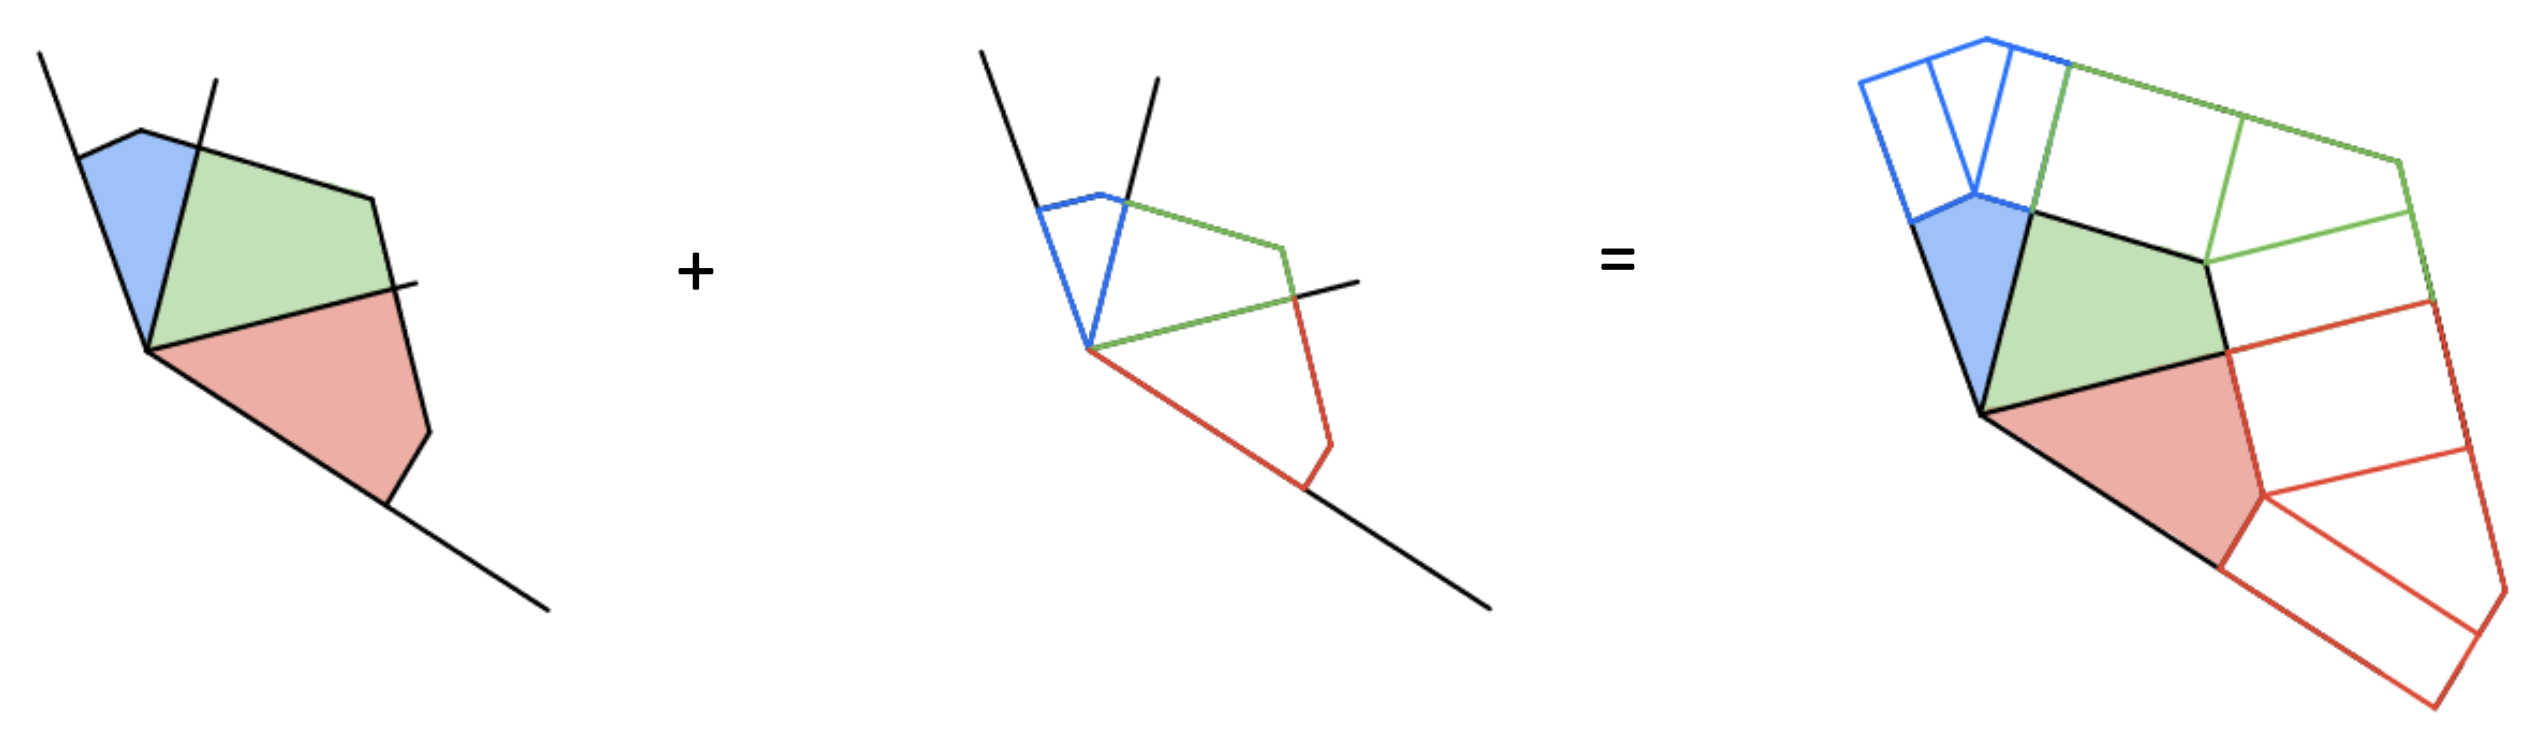
\includegraphics[width=1.05\textwidth]{./images/mvol_ex}
    \caption{Component wise Minkowski sums of two normal complexes of the same fan; note each polytope in the sum is still in its correct cone.}
\end{figure}
However, it is far from obvious that that this newly defined function will have any of the same nice properties of the original mixed volumes.
The development and proof of the following proposition was originally the work of Lauren Nowak in her master's thesis~\cite{nowakMixedVolumesNormal2022}, which goes much deeper into the volume theory that we are utilising.
The results were incorporated into our work with Nowak and Ross,~\cite[Proposition~3.1]{nowakMixedVolumesNormal2023}, which gives us the following guarantee.
\begin{proposition}
    Let \( \bSigma \subset \bN \) be a marked, simplicial \( d \)-fan, \( \ast \in \inn(\bN) \) an inner product, and pseudocubical values \( z_1, \dots, z_n \in \pCub(\bSigma, \ast)\).
    The function
    \[
        \MVol_{\bSigma, \ast}\,:\; \pCub(\bSigma, \ast)^d \to \R_{\geq 0}
    \]
    as defined above has the following properties:
    \begin{enumerate}
        \item \( \MVol_{\bSigma, \ast}(z, z, \dots, z) = \Vol_{\bSigma, \ast}(z) \),
        \item \( \MVol_{\bSigma, \ast} \) is symmetric in all arguments,
        \item \( \MVol_{\bSigma, \ast} \) is multilinear with respect to Minkowski addition in each maximal cone.
    \end{enumerate}

    Further, any function \( \pCub(\bSigma, \ast)^d \to \R_{\geq 0} \) satisfying properties 1--3 must be \( \MVol_{\sigma, \ast} \).
\end{proposition}
Our new mixed volume function then is well-defined and is uniquely characterized by essentially the same properties as the original mixed volume function.
Further,~\cite[Theorem~3.6]{nowakMixedVolumesNormal2023} provides an extension to \th\ref{thm:volDegCorrespondence} that links mixed volumes to the evaluation of mixed degrees of divisors.
\begin{theorem}\th\label{thm:mixedDeg}
    Let \( \bSigma \subset \bN \) be a balanced \( d \)-fan.
    Choose an inner product \( \ast \in \inn(\bN) \) and pseudocubical values \( z_1, \dots, z_d \in \pCub( \bSigma, \ast ) \).
    Then
    \[
        \MVol_{\bSigma, \ast}(z_1, \dots, z_d) = \deg\big( D(z_1) \cdots D(z_d) \big).
    \]
\end{theorem}
This is a successful bridge from the realm of geometry back to algebra.
We are now so close to having all the necessary components to prove our main result.
Not only do we have the link between geometry and algebra, it uses the concept of mixed volumes, which are closely related to log-concave sequences.
However, the Alexandrov--Fenchel inequality is, classically, very dependent on convexity, and normal complexes are, in general, decidedly non-convex.

\subsection{Amazing AF Fans}

If we take a fan at random, odds are high that we wouldn't see the mixed volumes of its normal complexes obey the Alexandrov--Fenchel inequality.
Unlike the convex setting, it is just generally not true.
However, one can find examples of fans such that the mixed volumes of their normal complex do obey the inequality.
This is in fact a property of the fan itself.
\begin{definition}[Alexandrov--Fenchel Property]\th\label{def:AF}
    Let \( \bSigma \subseteq \bN \) be a marked simplicial \( d \)-fan and \( \ast \in \inn(\bN) \) an inner product.
    We say that \( (\bSigma, \ast) \) is \emph{Alexandrov--Fenchel}, or just \emph{AF}, if \( \Cub(\bSigma, \ast) \neq \emptyset \) and
    \[
        \MVol_{\bSigma, \ast}(z_1, z_2, z_3, \dots, z_d)^2 \geq  \MVol_{\bSigma, \ast}(z_1, z_1, z_3, \dots, z_d)\MVol_{\bSigma, \ast}(z_2, z_2, z_3 \dots, z_d)
    \]
    for all \( z_1, z_2, z_3, \dots, z_d \in \Cub(\bSigma, \ast) \).
\end{definition}
If a fan is AF, then taking the mixed volumes of any normal complexes built from it will give rise to a log-concave sequence.
Our goal now is then to show that Bergman fans of matroids are AF, but we will need some way to prove that in general.
It is not feasible to check the Bergman fan of every matroid one by one.

Luckily, there is a way to more generally determine if a fan is AF\@.
Inspired by a strategy from a modern proof of the Alexandrov--Fenchel inequality, our work with Nowak and Ross showed a theorem,~\cite[Theorem~5.1]{nowakMixedVolumesNormal2023}, that gives us criteria to check.
We reproduce the theorem here.
\begin{theorem}[Nowak-O-Ross 2023]\th\label{thm:suffAF}
    Let \( \bSigma \subseteq \bN \) be a marked \( d \)-fan, and \( \ast \in \Inn(\bN) \) an inner product such that \( \Cub(\bSigma, \ast) \neq \emptyset \).
    Then \( (\bSigma, \ast) \) is AF if
    \begin{enumerate}[label=\roman*.]
        \item for every cone \( \sigma \in \bSigma(k) \), with \( k \leq d - 2 \),
              \[
                  \bSigma^\sigma \setminus \{ 0 \}
              \]
              is connected and,
        \item for every cone \( \sigma \in \bSigma(d-2) \), the volume polynomial of the star fan \( \Sigma^\sigma \) is a quadratic form whose associated matrix has exactly one positive eigenvalue.
    \end{enumerate}
\end{theorem}
We can provide a little insight into these two criteria.
In the first, connectedness is the classic topological definition of connected.
But, for those without a topological background, practically we can think of this as being able to draw a path between any two points in the star fans.
In this case, however they must remain connected when  the origin is removed.
The effect of this criterion is that it tells us our fans can't have ``pinch'' points.
If the cones of the fan share a non-0-dimensional face that is not a facet, then when taking stars within the fan we may get the case that the cones in the star fan meet only at the origin.
Once we then remove the origin, this will disconnect the star fan, violating the criterion.

For the second condition, let's quickly review quadratic forms.
A quadratic form is just a homogeneous polynomial of degree 2.
If \( p(x_1, \dots, x_n) \) is a quadratic form on \( n \) variables, then there exists an \( n \times n \) matrix \( A \) such that
\[
    p(x_1, \dots, x_n) = \vec{x}^T A \vec{x}
\]
where \( \vec{x}^T = \begin{bmatrix}
    x_1 \cdots x_n
\end{bmatrix} \).
Since we are looking at stars of \( (d - 2) \)-dimensional cones, the corresponding star fan will be a \( 2 \)-fan.
As we have seen, its volume polynomial \( \deg_{\bSigma^\sigma}(D(z)) \) will be a homogeneous polynomial of degree 2 in \( z \).
This second criterion is then a question of finding the signs of the eigenvalues of the matrix associated to each of these.

The inspiration for this proof comes from the paper, ``One more proof of the Alexandrov--Fenchel inequality'' \cite{cordero-erausquinOneMoreProof2019} which offers a proof of the Alexandrov--Fenchel inequalities in the classic convex setting.
This proof uses a dimension-reducing inductive argument on the volume of faces of polytopes.
This is why it was necessary to develop a notion of faces on normal complexes.
The first criterion of \th\ref{thm:suffAF} ensures that the faces of normal complexes meet a connectedness assumption that is needed in the inductive argument.
The second criterion is the base case, which in the convex setting is just always true but here must be shown per fan.

We now finally have laid out every piece of existing work we will need to prove our main result.
All that's left is to put them together.

\end{document}